\documentclass[8pt,apectratio=169]{beamer}

\usetheme[progressbar=frametitle]{metropolis}
\usepackage{appendixnumberbeamer}
\usepackage[style=authoryear, backend=bibtex8, natbib=true, maxcitenames=2]{biblatex}

\usepackage[utf8]{inputenc} % utf8x  defines more symbols, but may cause compatible problems
\usepackage{lmodern,textcomp} % Latin Modern fonts, contains €

\usepackage{graphicx}
\usepackage{import}

\usepackage{booktabs}
\usepackage[scale=2]{ccicons}

\usepackage{pgfplots}
\usepgfplotslibrary{dateplot}

\usepackage{xspace}
\newcommand{\themename}{\textbf{\textsc{metropolis}}\xspace}

% Math
\usepackage{amsmath}
\usepackage{bm} % bold symbol in math mode

% Optional packages
\usepackage{xcolor}
\usepackage{multicol}
\usepackage{hyperref}
\usepackage[super,negative]{nth} % allows writing 1st, 2nd, 3rd with superscript
\usepackage{ulem} % use the "sout" tag to "strikethrough" text
\usepackage{tcolorbox}

% Select what to do with command \comment:
  % \newcommand{\comment}[1]{}  %comments not shown
  % \newcommand{\comment}[1]{\par {\bfseries \color{blue} #1 \par}} %comments shown
% Select what to do with todonotes: i.e. \todo{}, \todo[inline]{}
  % \usepackage[disable]{todonotes} % notes not shown
  % \usepackage[draft]{todonotes}   % notes shown

%\numberwithin{equation}{section}

%\addbibresource{references}

\titlegraphic{\hfill 
\includegraphics[width=0.15 \textwidth]{figures/logo}}
\title{Microeconomics III, Ex. Class 4: Problem Set 1\footnote{Slides created for exercise class 4, with reservation for possible errors.\\}}
\author{Thor Donsby Noe (\href{mailto:thor.noe@econ.ku.dk}{thor.noe@econ.ku.dk})}
\date{September 11 2019} % \today
\institute{\normalsize Department of Economics, University of Copenhagen}

    % \definecolor{BlueTOL}{HTML}{222255}
    \definecolor{BrownTOL}{HTML}{666633}
    \definecolor{GreenTOL}{HTML}{225522}
    % \setbeamercolor{normal text}{fg=BlueTOL,bg=white}
    \setbeamercolor{alerted text}{fg=BrownTOL}
    \setbeamercolor{example text}{fg=GreenTOL}
    \setbeamercolor{background canvas}{bg=white}

    \setbeamercolor{block title alerted}{use=alerted text,
        fg=alerted text.fg,
        bg=alerted text.bg!80!alerted text.fg}
    \setbeamercolor{block body alerted}{use={block title alerted, alerted text},
        fg=alerted text.fg,
        bg=block title alerted.bg!50!alerted text.bg}
    \setbeamercolor{block title example}{use=example text,
        fg=example text.fg,
        bg=example text.bg!80!example text.fg}
    \setbeamercolor{block body example}{use={block title example, example text},
        fg=example text.fg,
        bg=block title example.bg!50!example text.bg}

\begin{document}
\maketitle

% ------------------------------------------------------------------------------
% ------ FRAME -----------------------------------------------------------------
% ------------------------------------------------------------------------------
\begin{frame}{Outline}
\tableofcontents
\end{frame}


\section{Kahoot!}

\begin{frame}{Kahoot: A exercises}
  Form a group for each table:
  \begin{itemize}
    \item Get prepared to answer the A exercises as a team (10 min).
  \end{itemize}
  
\includegraphics[width=\textwidth]{figures/kahoot}
\end{frame}


\section{PS3, Ex. 1 (A): Dominance and best response}

\begin{frame}{PS3, Ex. 1 (A): Dominance and best response}
  \begin{enumerate}
    \item (A) Show that for each of the following two games, the only Nash equilibrium is in pure strategies. Describe the intuition for this result. What do these two games have in common?
  \end{enumerate}
  \begin{multicols}{2}
    \begin{table}
      \begin{tabular}{cc|c|c|}
        & \multicolumn{1}{c}{} & \multicolumn{2}{c}{\color{blue}Player 2}\\
        \parbox[t]{1mm}{\multirow{3}{*}{\rotatebox[origin=r]{90}{\color{red}Player 1}}}
        & \multicolumn{1}{c}{} & \multicolumn{1}{c}{L}  & \multicolumn{1}{c}{\color{blue}R} \\\cline{3-4}
        & U & 5, 5 & 1, \textcolor{blue}{6}  \\\cline{3-4}
        & \color{red}D & \textcolor{red}{6}, 1 & \textcolor{red}{2}, \textcolor{blue}{2} \\\cline{3-4}
      \end{tabular}
    \end{table}
    $(D,R)$ is a unique Pure Strategy Nash Equilibrium (PSNE). The game is a Prisoner's Dilemma as it fulfills:
    \begin{align*}
      T>R>P>S\Leftrightarrow6>5>2>1
    \end{align*}
    i.e. the \textbf{T}emptation to deviate (6) is greater than the \textbf{R}eward for cooperating on the socially optimal outcome (5) and the \textbf{P}unishment payoff (2) is greater than the "\textbf{S}ucker's" payoff (1).
  \vfill\null \columnbreak
  \vfill\null
  \end{multicols}
\end{frame}
\begin{frame}{PS3, Ex. 1 (A): Dominance and best response}
  \begin{enumerate}
    \item (A) Show that for each of the following two games, the only Nash equilibrium is in pure strategies. Describe the intuition for this result. What do these two games have in common?
  \end{enumerate}
  \begin{multicols}{2}
    \begin{table}
      \begin{tabular}{cc|c|c|}
        & \multicolumn{1}{c}{} & \multicolumn{2}{c}{\color{blue}Player 2}\\
        \parbox[t]{1mm}{\multirow{3}{*}{\rotatebox[origin=r]{90}{\color{red}Player 1}}}
        & \multicolumn{1}{c}{} & \multicolumn{1}{c}{L}  & \multicolumn{1}{c}{\color{blue}R} \\\cline{3-4}
        & U & 5, 5 & 1, \textcolor{blue}{6}  \\\cline{3-4}
        & \color{red}D & \textcolor{red}{6}, 1 & \textcolor{red}{2}, \textcolor{blue}{2} \\\cline{3-4}
      \end{tabular}
    \end{table}
    $(D,R)$ is a unique Pure Strategy Nash Equilibrium (PSNE). The game is a Prisoner's Dilemma as it fulfills:
    \begin{align*}
      T>R>P>S\Leftrightarrow6>5>2>1
    \end{align*}
    i.e. the \textbf{T}emptation to deviate (6) is greater than the \textbf{R}eward for cooperating on the socially optimal outcome (5) and the \textbf{P}unishment payoff (2) is greater than the "\textbf{S}ucker's" payoff (1).
  \vfill\null \columnbreak
    \begin{table}
      \begin{tabular}{cc|c|c|c|}
        & \multicolumn{1}{c}{} & \multicolumn{3}{c}{\color{blue}Player 2}\\
        \parbox[t]{1mm}{\multirow{3}{*}{\rotatebox[origin=r]{90}{\color{red}Player 1}}}
        & \multicolumn{1}{c}{} & \multicolumn{1}{c}{L} & \multicolumn{1}{c}{C} & \multicolumn{1}{c}{R} \\\cline{3-5}
        & U & \textcolor{red}{1}, 0 & \textcolor{red}{1}, \textcolor{blue}{2} & 0, 1 \\\cline{3-5}
        & D & 0, \textcolor{blue}{3} & 0, 1 & \textcolor{red}{2}, 0 \\\cline{3-5}
      \end{tabular}
    \end{table}
    $(U,C)$ is a unique Pure Strategy Nash Equilibrium (PSNE) as no other combination of (mixed or pure) strategies gives as high payoffs.\\\medskip
    Iterated Elimination of Strictly Dominated Strategies (IESDS) leads to the same outcome as the best responses (eliminate $R$ then $D$ and lastly $L$).
  \vfill\null
  \end{multicols}
\end{frame}
\begin{frame}{PS3, Ex. 1 (A): Dominance and best response}
  \begin{enumerate}
    \item (A) Show that for each of the following two games, the only Nash equilibrium is in pure strategies. Describe the intuition for this result. What do these two games have in common?
  \end{enumerate}
  \begin{multicols}{2}
    \begin{table}
      \begin{tabular}{cc|c|c|}
        & \multicolumn{1}{c}{} & \multicolumn{2}{c}{\color{blue}Player 2}\\
        \parbox[t]{1mm}{\multirow{3}{*}{\rotatebox[origin=r]{90}{\color{red}Player 1}}}
        & \multicolumn{1}{c}{} & \multicolumn{1}{c}{L}  & \multicolumn{1}{c}{\color{blue}R} \\\cline{3-4}
        & U & 5, 5 & 1, \textcolor{blue}{6}  \\\cline{3-4}
        & \color{red}D & \textcolor{red}{6}, 1 & \textcolor{red}{2}, \textcolor{blue}{2} \\\cline{3-4}
      \end{tabular}
    \end{table}
    $(D,R)$ is a unique Pure Strategy Nash Equilibrium (PSNE). The game is a Prisoner's Dilemma as it fulfills:
    \begin{align*}
      T>R>P>S\Leftrightarrow6>5>2>1
    \end{align*}
    i.e. the \textbf{T}emptation to deviate (6) is greater than the \textbf{R}eward for cooperating on the socially optimal outcome (5) and the \textbf{P}unishment payoff (2) is greater than the "\textbf{S}ucker's" payoff (1).
  \vfill\null \columnbreak
    \begin{table}
      \begin{tabular}{cc|c|c|c|}
        & \multicolumn{1}{c}{} & \multicolumn{3}{c}{\color{blue}Player 2}\\
        \parbox[t]{1mm}{\multirow{3}{*}{\rotatebox[origin=r]{90}{\color{red}Player 1}}}
        & \multicolumn{1}{c}{} & \multicolumn{1}{c}{L} & \multicolumn{1}{c}{C} & \multicolumn{1}{c}{R} \\\cline{3-5}
        & U & \textcolor{red}{1}, 0 & \textcolor{red}{1}, \textcolor{blue}{2} & 0, 1 \\\cline{3-5}
        & D & 0, \textcolor{blue}{3} & 0, 1 & \textcolor{red}{2}, 0 \\\cline{3-5}
      \end{tabular}
    \end{table}
    $(U,C)$ is a unique Pure Strategy Nash Equilibrium (PSNE) as no other combination of (mixed or pure) strategies gives as high payoffs.\\\medskip
    Iterated Elimination of Strictly Dominated Strategies (IESDS) leads to the same outcome as the best responses (eliminate $R$ then $D$ and lastly $L$).
  \vfill\null
  \end{multicols}
  \vspace{-20pt}
  In a mixed strategy NE both players must be indifferent between their respective pure strategies. This is impossible if one of the strategies are strictly dominated.\\\medskip
  \textbf{As both games can be solved by IESDS they both have a unique PSNE.}
\end{frame}


\section{PS3, Ex. 2 (A): Equilibrium selection}

\begin{frame}{PS3, Ex. 2 (A): Equilibrium selection}
  \begin{itemize}
    \item[2.] (A) Solve for all pure strategy Nash equilibria. Which equilibrium do you find most reasonable?
  \end{itemize}
  \begin{multicols}{2}
    \begin{table}
      \begin{tabular}{cc|c|c|c|}
        & \multicolumn{1}{c}{} & \multicolumn{3}{c}{\color{blue}Player 2}\\
        & \multicolumn{1}{c}{} & \multicolumn{1}{c}{a} & \multicolumn{1}{c}{b} & \multicolumn{1}{c}{c} \\\cline{3-5}
        \parbox[t]{1mm}{\multirow{3}{*}{\rotatebox[origin=c]{90}{\color{red}Player 1}}}
        & A & \textcolor{red}{2}, \textcolor{blue}{2} & \textcolor{red}{0}, 0 & -1, \textcolor{blue}{2} \\\cline{3-5}
        & B & 0, \textcolor{blue}{0} & \textcolor{red}{0}, \textcolor{blue}{0} & 0, \textcolor{blue}{0} \\\cline{3-5}
        & C & \textcolor{red}{2}, -1 & \textcolor{red}{0}, 0 & \textcolor{red}{1}, \textcolor{blue}{1} \\\cline{3-5}
      \end{tabular}
    \end{table}
    $PSNE=\{(A,a),(B,b),(C,c)\}$.
  \vfill\null \columnbreak
  \vfill\null
  \end{multicols}
\end{frame}
\begin{frame}{PS3, Ex. 2 (A): Equilibrium selection}
  \begin{itemize}
    \item[2.] (A) Solve for all pure strategy Nash equilibria. Which equilibrium do you find most reasonable?
  \end{itemize}
  \begin{multicols}{2}
    \begin{table}
      \begin{tabular}{cc|c|c|c|}
        & \multicolumn{1}{c}{} & \multicolumn{3}{c}{\color{blue}Player 2}\\
        & \multicolumn{1}{c}{} & \multicolumn{1}{c}{a} & \multicolumn{1}{c}{b} & \multicolumn{1}{c}{c} \\\cline{3-5}
        \parbox[t]{1mm}{\multirow{3}{*}{\rotatebox[origin=c]{90}{\color{red}Player 1}}}
        & A & \textcolor{red}{2}, \textcolor{blue}{2} & \textcolor{red}{0}, 0 & -1, \textcolor{blue}{2} \\\cline{3-5}
        & B & 0, \textcolor{blue}{0} & \textcolor{red}{0}, \textcolor{blue}{0} & 0, \textcolor{blue}{0} \\\cline{3-5}
        & C & \textcolor{red}{2}, -1 & \textcolor{red}{0}, 0 & \textcolor{red}{1}, \textcolor{blue}{1} \\\cline{3-5}
      \end{tabular}
    \end{table}
    $PSNE=\{(A,a),(B,b),(C,c)\}$.
  \vfill\null \columnbreak
    For \textbf{risk neutral} players $(A,a)$ is the most reasonable as it maximizes payoff for both players.\\\medskip
    For \textbf{risk averse} players avoiding $A$ and $a$ eliminates the risk of a negative payoff. $(C,c)$ is more reasonable than $(B,b)$ as the payoffs are positive.
  \vfill\null
  \end{multicols}
\end{frame}


\section{PS3, Ex. 3 (A): NE proof using IEWDS}

\begin{frame}{PS3, Ex. 3 (A): NE proof using IEWDS}
  \begin{itemize}
    \item[3.] (A)  We have seen in the lectures that IESDS never eliminates a Nash Equilibrium. However, we saw in Problem Set 2 that this is not true if we do iterated elimination of weakly dominated strategies (IEWDS.) Go through the proof in the slides from lecture 2 and identify the step that is no longer true if we replace IESDS by IEWDS. That is, explain why the proof is no longer true when we replace ‘strict domination’ by ‘weak domination’.
  \end{itemize}
  \begin{multicols}{2}
  \vfill\null \columnbreak
  \vfill\null
  \end{multicols}
\end{frame}
\begin{frame}{PS3, Ex. 3 (A): NE proof using IEWDS}
  \textbf{Informal proof:} For the intuition, look at this example for now. At home, you can compare the two different formal proofs.
  \begin{multicols}{2}
    \begin{table}
      \begin{tabular}{cc|c|c|}
        & \multicolumn{1}{c}{} & \multicolumn{2}{c}{\color{blue}Player 2}\\
        \parbox[t]{1mm}{\multirow{3}{*}{\rotatebox[origin=r]{90}{\color{red}Player 1}}}
        & \multicolumn{1}{c}{} & \multicolumn{1}{c}{L}  & \multicolumn{1}{c}{R} \\\cline{3-4}
        & U & \textcolor{red}{3}, \textcolor{blue}{2} & 0, 0  \\\cline{3-4}
        & D & \textcolor{red}{3}, 0 & \textcolor{red}{1}, \textcolor{blue}{2} \\\cline{3-4}
      \end{tabular}
    \end{table}
    \textbf{NE} is any strategy where no player can be strictly better off by deviating:
    \begin{align*}
      NE=\{(U,L),(D,R)\}
    \end{align*}
  \vfill\null\columnbreak
  \vfill\null
  \end{multicols}
\end{frame}
\begin{frame}{PS3, Ex. 3 (A): NE proof using IEWDS}
  \textbf{Informal proof:} For the intuition, look at this example for now. At home, you can compare the two different formal proofs.
  \begin{multicols}{2}
    \begin{table}
      \begin{tabular}{cc|c|c|}
        & \multicolumn{1}{c}{} & \multicolumn{2}{c}{\color{blue}Player 2}\\
        \parbox[t]{1mm}{\multirow{3}{*}{\rotatebox[origin=r]{90}{\color{red}Player 1}}}
        & \multicolumn{1}{c}{} & \multicolumn{1}{c}{L}  & \multicolumn{1}{c}{R} \\\cline{3-4}
        & U & \textcolor{red}{3}, \textcolor{blue}{2} & 0, 0  \\\cline{3-4}
        & D & \textcolor{red}{3}, 0 & \textcolor{red}{1}, \textcolor{blue}{2} \\\cline{3-4}
      \end{tabular}
    \end{table}
    \textbf{NE} is any strategy where no player can be strictly better off by deviating:
    \begin{align*}
      NE=\{(U,L),(D,R)\}
    \end{align*}
    \textbf{IESDS:} If a strategy was strongly dominated there would be a clear incentive to deviate from it, thus, by definition the strategy could not be a NE.
  \vfill\null\columnbreak
  \vfill\null
  \end{multicols}
\end{frame}
\begin{frame}{PS3, Ex. 3 (A): NE proof using IEWDS}
  \textbf{Informal proof:} For the intuition, look at this example for now. At home, you can compare the two different formal proofs.
  \begin{multicols}{2}
    \begin{table}
      \begin{tabular}{cc|c|c|}
        & \multicolumn{1}{c}{} & \multicolumn{2}{c}{\color{blue}Player 2}\\
        \parbox[t]{1mm}{\multirow{3}{*}{\rotatebox[origin=r]{90}{\color{red}Player 1}}}
        & \multicolumn{1}{c}{} & \multicolumn{1}{c}{L}  & \multicolumn{1}{c}{R} \\\cline{3-4}
        & U & \textcolor{red}{3}, \textcolor{blue}{2} & 0, 0  \\\cline{3-4}
        & D & \textcolor{red}{3}, 0 & \textcolor{red}{1}, \textcolor{blue}{2} \\\cline{3-4}
      \end{tabular}
    \end{table}
    \textbf{NE} is any strategy where no player can be strictly better off by deviating:
    \begin{align*}
      NE=\{(U,L),(D,R)\}
    \end{align*}
    \textbf{IESDS:} If a strategy was strongly dominated there would be a clear incentive to deviate from it, thus, by definition the strategy could not be a NE.
  \vfill\null\columnbreak
  \textbf{IEWDS:} In a NE where a player $1$ is indifferent between the NE-payoff and her payoff from deviating, the NE-strategy can be weakly dominated if player $1$'s' alternative strategy would give a higher payoff in the case where player $2$ deviates from his NE strategy as well.
  \vfill\null
  \end{multicols}
\end{frame}
\begin{frame}{PS3, Ex. 3 (A): NE proof using IEWDS}
  \textbf{Informal proof:} For the intuition, look at this example for now. At home, you can compare the two different formal proofs.
  \begin{multicols}{2}
    \begin{table}
      \begin{tabular}{cc|c|c|}
        & \multicolumn{1}{c}{} & \multicolumn{2}{c}{\color{blue}Player 2}\\
        \parbox[t]{1mm}{\multirow{3}{*}{\rotatebox[origin=r]{90}{\color{red}Player 1}}}
        & \multicolumn{1}{c}{} & \multicolumn{1}{c}{L}  & \multicolumn{1}{c}{R} \\\cline{3-4}
        & \sout{U} & \sout{\textcolor{red}{3}, \textcolor{blue}{2}} & \sout{0, 0}  \\\cline{3-4}
        & D & \textcolor{red}{3}, 0 & \textcolor{red}{1}, \textcolor{blue}{2} \\\cline{3-4}
      \end{tabular}
    \end{table}
    \textbf{NE} is any strategy where no player can be strictly better off by deviating:
    \begin{align*}
      NE=\{(U,L),(D,R)\}
    \end{align*}
    \textbf{IESDS:} If a strategy was strongly dominated there would be a clear incentive to deviate from it, thus, by definition the strategy could not be a NE.
  \vfill\null\columnbreak
    \textbf{IEWDS:} In a NE where a player $1$ is indifferent between the NE-payoff and her payoff from deviating, the NE-strategy can be weakly dominated if player $1$'s' alternative strategy would give a higher payoff in the case where player $2$ deviates from his NE strategy as well.\\\medskip
    E.g. Player 1 is indifferent between $u_1(U,L)$ and $u_1(D,L)$, however, $u_1(D,R)>u_1(U,R)$, i.e. $D$ weakly dominates $U$ and $U$ can be eliminated. I.e. eliminating the NE $(U,L)$, leaving behind the reduced form game:
    \begin{table}
      \begin{tabular}{cc|c|c|}
        & \multicolumn{1}{c}{} & \multicolumn{2}{c}{\color{blue}Player 2}\\
        \parbox[t]{1mm}{\multirow{2}{*}{\rotatebox[origin=c]{90}{\color{red}Player 1}}}
        & \multicolumn{1}{c}{} & \multicolumn{1}{c}{L}  & \multicolumn{1}{c}{R} \\\cline{3-4}
        & D & \textcolor{red}{3}, 0 & \textcolor{red}{1}, \textcolor{blue}{2} \\\cline{3-4}
      \end{tabular}
    \end{table}
  \vfill\null
  \end{multicols}
\end{frame}
\begin{frame}{PS3, Ex. 3 (A): NE proof using IEWDS}
    \textbf{Formal proof:} The proof that all NE survive IESDS holds by contradiction. For the two-player case the IESDS proof is as follows:
  \begin{multicols}{2}
    \begin{itemize}
      \item Let $(s_1^{*},s_2^{*})$ be a NE.
      \item Say we carry out IESDS and $s_1^{*}$ is the first NE strategy to be eliminated (in round $n$ of elimination).
      \item Then there must be a strategy $s_1^{'}\neq s_1^{*}$ that strictly dominates $s_1^{*}$, i.e.
    \end{itemize}
      \begin{align}
        \forall s_2\in S_2^n:\ u_1(s_1^{*},s_2)<u_1(s_1^{'},s_2)\label{iesds}
      \end{align}
      \begin{itemize}
        \item[] where $S_2^n$ is the set of player-2 strategies that have not been eliminated in rounds $1,...,n-1$.
      \end{itemize}
  \vfill\null\columnbreak
    \begin{itemize}
      \item Since $s_2^{*}\in S_2^n$, inequality \eqref{iesds} also means
      \begin{align*}
        u_1(s_1^{*},s_2^{*})<u_1(s_1^{'},s_2^{*})
      \end{align*}
      \item But $(s_1^{*},s_2^{*})$ is a NE, so by definition
      \begin{align*}
        \forall s_1\in S_1:\ u_1(s_1^{*},s_2^{*})\geq u_1(s_1,s_2^{*})
      \end{align*}
      \item Contradiction! We can do the same for player 2. It follows that $s_i^{*}$ survives IESDS for $i=1,2$.
    \end{itemize}
  \vfill\null
  \end{multicols}
\end{frame}
% \begin{frame}{PS3, Ex. 3 (A): NE proof using IEWDS}
%     \textbf{Formal proof:} The proof that all NE survive IESDS holds by contradiction. We \underline{\textbf{highlight}} where the contradiction breaks down using IEWDS instead:
%   \begin{multicols}{2}
%     \begin{itemize}
%       \item Let $(s_1^{*},s_2^{*})$ be a NE.
%       \item Say we carry out \underline{\textbf{IEWDS}} and $s_1^{*}$ is the first NE strategy to be eliminated (in round $n$ of elimination).
%       \item Then there must be a strategy $s_1^{'}\neq s_1^{*}$ that \underline{\textbf{weakly}} dominates $s_1^{*}$, i.e.
%     \end{itemize}
%       \begin{align*}
%         \forall s_2\in S_2^n:\ u_1(s_1^{*},s_2)\underbrace{\bm{\leq}}_\text{\underline{\textbf{Weak}}}u_1(s_1^{'},s_2)
%       \end{align*}
%       \begin{itemize}
%         \item[] \underline{\textbf{and the inequality holds strictly for}} \underline{\textbf{at least one strategy $\bm{s_2^{'}\in S_2^n}$}} where $S_2^n$ is the set of player-2 strategies that have not been eliminated in rounds $1,...,n-1$.
%       \end{itemize}
%   \vfill\null \columnbreak
%   \vfill\null
%   \end{multicols}
% \end{frame}
\begin{frame}{PS3, Ex. 3 (A): NE proof using IEWDS}
    \textbf{Formal proof:} The proof that all NE survive IESDS holds by contradiction. We \underline{\textbf{highlight}} where the contradiction breaks down using IEWDS instead:
  \begin{multicols}{2}
    \begin{itemize}
      \item Let $(s_1^{*},s_2^{*})$ be a NE.
      \item Say we carry out \underline{\textbf{IEWDS}} and $s_1^{*}$ is the first NE strategy to be eliminated (in round $n$ of elimination).
      \item Then there must be a strategy $s_1^{'}\neq s_1^{*}$ that \underline{\textbf{weakly}} dominates $s_1^{*}$, i.e.
    \end{itemize}
      \begin{align}
        \forall s_2\in S_2^n:\ u_1(s_1^{*},s_2)\underbrace{\bm{\leq}}_\text{\underline{\textbf{Weak}}}u_1(s_1^{'},s_2)\label{iewds}
      \end{align}
      \begin{itemize}
        \item[] \underline{\textbf{and the inequality holds strictly for}} \underline{\textbf{at least one strategy $\bm{s_2^{'}\in S_2^n}$}} where $S_2^n$ is the set of player-2 strategies that have not been eliminated in rounds $1,...,n-1$.
      \end{itemize}
  \vfill\null\columnbreak
    \begin{itemize}
      \item Since $s_2^{*}\in S_2^n$, inequality \eqref{iewds} also means
      \begin{align*}
        u_1(s_1^{*},s_2^{*})\underbrace{\bm{\leq}}_\text{\underline{\textbf{Weak}}}u_1(s_1^{'},s_2^{*})
      \end{align*}
      \item \sout{But} $(s_1^{*},s_2^{*})$ is a NE, so by definition
      \begin{align*}
        \forall s_1\in S_1:\ u_1(s_1^{*},s_2^{*})\geq u_1(s_1,s_2^{*})
      \end{align*}
      \item \underline{\textbf{No}} contradiction!
    \end{itemize}
    \underline{\textbf{Conclusion}}: for a NE $(s_1^{*},s_2^{*})$ IEWDS can eliminate $s_1^{*}$ if $s_1^{'},s_2^{'}$ exist such that:
    \begin{align*}
      \text{for }s_1^{'}\in S_1^n:\ u_1(s_1^{*},s_2^{*})=u_1(s_1^{'},s_2^{*})
    \end{align*}
    and
    \begin{align*}
      \text{for }s_2^{'}\in S_2^n:\ u_1(s_1^{*},s_2^{'})<u_1(s_1^{'},s_2^{'})
    \end{align*}
  \vfill\null
  \end{multicols}
\end{frame}


\section{PS3, Ex. 4 (A): Mixed strategy price competition}

\begin{frame}{PS3, Ex. 4 (A): Mixed strategy price competition}
    \begin{itemize}
      \item[4.] (A). Consider price competition between two firms when some consumers are informed about prices and others are not. Firms have zero marginal cost and they set price simultaneously; for the sake of this example, assume each price can only take one of the following values: 80, 54, 38. The market consists of two consumers. The uninformed consumer will visit a firm at random (probabilities $\frac{1}{2},\frac{1}{2}$) and buy from it, regardless of the price. The informed consumer will visit the firm with the lowest price and buy from it. If both firms set the same price, assume that the informed consumer picks a firm at random (probabilities $\frac{1}{2},\frac{1}{2}$).
      \item[(a)] Argue that this game can be represented by the following bimatrix.
      \vspace{-4pt}
      \begin{table}
        \begin{tabular}{c|c|c|c|}
          \multicolumn{1}{c}{} & \multicolumn{1}{c}{$p_2$=80} & \multicolumn{1}{c}{$p_2$=54} & \multicolumn{1}{c}{$p_2$=38} \\\cline{2-4}
          $p_1$=80 & 80, 80 & 40, 81 & 40, 57 \\\cline{2-4}
          $p_1$=54 & 81, 40 & 54, 54 & 27, 57 \\\cline{2-4}
          $p_1$=38 & 57, 40 & 57, 27 & 38, 38 \\\cline{2-4}
        \end{tabular}
      \end{table}
      \item[(b)] Show that there is no Nash equilibrium in pure strategies.
      \item[(c)] Confirm that the following strategy profile is a Nash equilibrium: each firm plays price 80 with probability 0.232, price 54 with probability 0.361, and price 38 with probability 0.407.
      \item[(d)] Why do you think the equilibrium is so different from the standard Bertrand pricing game (i.e. where competition drives price down to marginal cost)?
    \end{itemize}
\end{frame}
\begin{frame}{PS3, Ex. 4 (A): Mixed strategy price competition}
    \begin{itemize}
      \item[(a)] The game in normal form and bimatrix:
    \end{itemize}
    Players: \textit{Firm 1, Firm 2}. Strategies: $p_i\in S_i = S = \{80, 54, 38\}$\\\medskip
    Payoffs consist of \textit{payoff from the informed consumer} + \textit{payoff from the uninformed}.
    I.e. payoffs for player $i\neq j$:
    \begin{align*}
      u_i(p_i,p_j)=
      \left\{ \begin{array}{rcl}
      p_i + \frac{1}{2}p_i & \mbox{if} & p_i < p_j \\
      \frac{1}{2}p_i + \frac{1}{2}p_i & \mbox{if} & p_i = p_j \\
      0 + \frac{1}{2}p_i & \mbox{if} & p_i > p_j
      \end{array}\right.
    \end{align*}
  \vfill\null
\end{frame}
\begin{frame}{PS3, Ex. 4 (A): Mixed strategy price competition}
    \begin{itemize}
      \item[(a)] The game in normal form and bimatrix:
    \end{itemize}
    Players: \textit{Firm 1, Firm 2}. Strategies: $p_i\in S_i = S = \{80, 54, 38\}$\\\medskip
    Payoffs consist of \textit{payoff from the informed consumer} + \textit{payoff from the uninformed}.
    I.e. payoffs for player $i\neq j$:
    \begin{align*}
      u_i(p_i,p_j)=
      \left\{ \begin{array}{rcl}
      p_i + \frac{1}{2}p_i & \mbox{if} & p_i < p_j \\
      \frac{1}{2}p_i + \frac{1}{2}p_i & \mbox{if} & p_i = p_j \\
      0 + \frac{1}{2}p_i & \mbox{if} & p_i > p_j
      \end{array}\right.
      =
      \left\{ \begin{array}{rcl}
      \frac{3}{2}p_i & \mbox{if} & p_i < p_j \\
                 p_i & \mbox{if} & p_i = p_j \\
      \frac{1}{2}p_i & \mbox{if} & p_i > p_j
      \end{array}\right.
    \end{align*}
  \vfill\null
\end{frame}
\begin{frame}{PS3, Ex. 4 (A): Mixed strategy price competition}
    \begin{itemize}
      \item[(a)] The game in normal form and bimatrix:
    \end{itemize}
    Players: \textit{Firm 1, Firm 2}. Strategies: $p_i\in S_i = S = \{80, 54, 38\}$\\\medskip
    Payoffs consist of \textit{payoff from the informed consumer} + \textit{payoff from the uninformed}.
    I.e. payoffs for player $i\neq j$:
    \begin{align*}
      u_i(p_i,p_j)=
      \left\{ \begin{array}{rcl}
      p_i + \frac{1}{2}p_i & \mbox{if} & p_i < p_j \\
      \frac{1}{2}p_i + \frac{1}{2}p_i & \mbox{if} & p_i = p_j \\
      0 + \frac{1}{2}p_i & \mbox{if} & p_i > p_j
      \end{array}\right.
      =
      \left\{ \begin{array}{rcl}
      \frac{3}{2}p_i & \mbox{if} & p_i < p_j \\
                 p_i & \mbox{if} & p_i = p_j \\
      \frac{1}{2}p_i & \mbox{if} & p_i > p_j
      \end{array}\right.
    \end{align*}
    Which can be represented as:
      \vspace{-6pt}
      \begin{table}
        \begin{tabular}{c|c|c|c|}
          \multicolumn{1}{c}{} & \multicolumn{1}{c}{$p_j$=80} & \multicolumn{1}{c}{$p_j$=54} & \multicolumn{1}{c}{$p_j$=38} \\\cline{2-4}
          $p_i$=80 & 80, - & $\frac{1}{2}$80=40, - & $\frac{1}{2}$80=40, - \\\cline{2-4}
          $p_i$=54 & $\frac{3}{2}$54=81, - & 54, - & $\frac{1}{2}$54=27, - \\\cline{2-4}
          $p_i$=38 & $\frac{3}{2}$80=57, - & $\frac{3}{2}$38=57, - & 38, - \\\cline{2-4}
        \end{tabular}
      \end{table}
  \vfill\null
\end{frame}
\begin{frame}{PS3, Ex. 4 (A): Mixed strategy price competition}
    \begin{itemize}
      \item[(a)] The game in normal form and bimatrix:
    \end{itemize}
    Players: \textit{Firm 1, Firm 2}. Strategies: $p_i\in S_i = S = \{80, 54, 38\}$\\\medskip
    Payoffs consist of \textit{payoff from the informed consumer} + \textit{payoff from the uninformed}.
    I.e. payoffs for player $i\neq j$:
    \begin{align*}
      u_i(p_i,p_j)=
      \left\{ \begin{array}{rcl}
      p_i + \frac{1}{2}p_i & \mbox{if} & p_i < p_j \\
      \frac{1}{2}p_i + \frac{1}{2}p_i & \mbox{if} & p_i = p_j \\
      0 + \frac{1}{2}p_i & \mbox{if} & p_i > p_j
      \end{array}\right.
      =
      \left\{ \begin{array}{rcl}
      \frac{3}{2}p_i & \mbox{if} & p_i < p_j \\
                 p_i & \mbox{if} & p_i = p_j \\
      \frac{1}{2}p_i & \mbox{if} & p_i > p_j
      \end{array}\right.
    \end{align*}
    Which can be represented as:
      \vspace{-6pt}
      \begin{table}
        \begin{tabular}{c|c|c|c|}
          \multicolumn{1}{c}{} & \multicolumn{1}{c}{$p_j$=80} & \multicolumn{1}{c}{$p_j$=54} & \multicolumn{1}{c}{$p_j$=38} \\\cline{2-4}
          $p_i$=80 & 80, - & $\frac{1}{2}$80=40, - & $\frac{1}{2}$80=40, - \\\cline{2-4}
          $p_i$=54 & $\frac{3}{2}$54=81, - & 54, - & $\frac{1}{2}$54=27, - \\\cline{2-4}
          $p_i$=38 & $\frac{3}{2}$80=57, - & $\frac{3}{2}$38=57, - & 38, - \\\cline{2-4}
        \end{tabular}
      \end{table}
    \begin{itemize}
      \item[(b)] Show that there is no Nash equilibrium in pure strategies:
    \end{itemize}
    \vspace{-4pt}
    \begin{table}
      \begin{tabular}{cc|c|c|c|}
        & \multicolumn{1}{c}{} & \multicolumn{3}{c}{\color{blue}Firm 2}\\
        & \multicolumn{1}{c}{} & \multicolumn{1}{c}{$p_2$=80} & \multicolumn{1}{c}{$p_2$=54} & \multicolumn{1}{c}{$p_2$=38} \\\cline{3-5}
        \parbox[t]{1mm}{\multirow{3}{*}{\rotatebox[origin=c]{90}{\color{red}Firm 1}}}
        & $p_1$=80 & 80, 80 & 40, \textcolor{blue}{81} & \textcolor{red}{40}, 57 \\\cline{3-5}
        & $p_1$=54 & \textcolor{red}{81}, 40 & 54, 54 & 27, \textcolor{blue}{57} \\\cline{3-5}
        & $p_1$=38 & 57, \textcolor{blue}{40} & \textcolor{red}{57}, 27 & 38, 38 \\\cline{3-5}
      \end{tabular}
    \end{table}
  \vfill\null
\end{frame}
\begin{frame}{PS3, Ex. 4 (A): Mixed strategy price competition}
    \begin{itemize}
      \item[(c)] Confirm that the following strategy profile is a Nash equilibrium: each firm plays price 80 with probability 0.232, price 54 with probability 0.361, and price 38 with probability 0.407.
    \end{itemize}
    \begin{tabular}{|l|}
      \cline{1-1}
      \textbf{Remember}: In an equilibrium in mixed strategies, a player is indifferent between all \\
      pure strategies that she is choosing with positive probability.\\\cline{1-1}
    \end{tabular}
    \begin{table}
      \begin{tabular}{c|c|c|c|}
        \multicolumn{1}{c}{} & \multicolumn{1}{c}{$p_2$=80} & \multicolumn{1}{c}{$p_2$=54} & \multicolumn{1}{c}{$p_2$=38} \\\cline{2-4}
        $p_1$=80 & 80, 80 & 40, 81 & 40, 57 \\\cline{2-4}
        $p_1$=54 & 81, 40 & 54, 54 & 27, 57 \\\cline{2-4}
        $p_1$=38 & 57, 40 & 57, 27 & 38, 38 \\\cline{2-4}
      \end{tabular}
    \end{table}
  \vfill\null
\end{frame}
\begin{frame}{PS3, Ex. 4 (A): Mixed strategy price competition}
    \begin{itemize}
      \item[(c)] Confirm that the following strategy profile is a Nash equilibrium: each firm plays price 80 with probability 0.232, price 54 with probability 0.361, and price 38 with probability 0.407.
    \end{itemize}
    \begin{tabular}{|l|}
      \cline{1-1}
      \textbf{Remember}: In an equilibrium in mixed strategies, a player is indifferent between all \\
      pure strategies that she is choosing with positive probability.\\\cline{1-1}
    \end{tabular}
    \begin{table}
      \begin{tabular}{c|c|c|c|}
        \multicolumn{1}{c}{} & \multicolumn{1}{c}{$p_2$=80} & \multicolumn{1}{c}{$p_2$=54} & \multicolumn{1}{c}{$p_2$=38} \\\cline{2-4}
        $p_1$=80 & 80, 80 & 40, 81 & 40, 57 \\\cline{2-4}
        $p_1$=54 & 81, 40 & 54, 54 & 27, 57 \\\cline{2-4}
        $p_1$=38 & 57, 40 & 57, 27 & 38, 38 \\\cline{2-4}
      \end{tabular}
    \end{table}
    Check that firm $i$ is indifferent between all pure strategies when the opposing firm's strategy is given by the probability distribution $\widehat{p_j}=(0.232,0.361)$:
    \begin{align*}
      u_i(p_i=80,\widehat{p_j})= 0.232\cdot80 + 0.361\cdot40 + (1-0.232-0.361)\cdot40 = 49.280 \approx 49.3\\
      u_i(p_i=54,\widehat{p_j})= 0.232\cdot81 + 0.361\cdot54 + (1-0.232-0.361)\cdot27 = 49.275 \approx 49.3\\
      u_i(p_i=38,\widehat{p_j})= 0.232\cdot57 + 0.361\cdot57 + (1-0.232-0.361)\cdot38 = 49.267 \approx 49.3
    \end{align*}
    There are rounding errors as the exact mixed strategy profile is $\widehat{p_j}=\left(\frac{193}{833},\frac{8127}{22491}\right)$.
  \vfill\null
\end{frame}
\begin{frame}{PS3, Ex. 4 (A): Mixed strategy price competition}
    \begin{itemize}
      \item[(d)] Why do you think the equilibrium is so different from the standard Bertrand pricing game (i.e. where competition drives price down to marginal cost)?
    \end{itemize}
  \vfill\null
\end{frame}
\begin{frame}{PS3, Ex. 4 (A): Mixed strategy price competition}
    \begin{itemize}
      \item[(d)] Why do you think the equilibrium is so different from the standard Bertrand pricing game (i.e. where competition drives price down to marginal cost)?
    \end{itemize}
    In the standard Bertrand Oligopoly price competition would lead to the perfectly competitive outcome (price = marginal cost), here:
    \begin{align*}
      p_1^{*}=p_2^{*}=c=0
    \end{align*}
    Introduction of an uninformed consumer dampens the effect of price competition as a firm $i$ can expect a revenue of at least $\frac{1}{2}p_i$ no matter what price $p_i$ it sets.\\\medskip
    Price competition could be increased by lowering the probability that an uninformed customer randomly picks the firm, i.e. through:
    \begin{enumerate}
      \item A higher share of informed customers.
      \item More competing firms (however, other effects affect the outcome as well).
    \end{enumerate}
  \vfill\null
\end{frame}


\section{PS4, Ex. 2: Entry deterrence in a game tree}

\begin{frame}{PS4, Ex. 2: Entry deterrence in a game tree}
  \begin{multicols}{2}
    Consider the following dynamic game: firm 1 owns a shop in town A. Firm 2 decides whether to enter the market in town A. If firm 2 enters, firm 1 chooses whether to fight or accommodate the entrant. If firm 2 does not enter, firm 1 receives a profit of 2 and firm 2 gets 0. If firm 2 enters and firm 1 accommodates, they share the market and each of them receives a profit of 1. If firm 2 enters and firm 1 decides to fight, firm 2 suffers a loss of 1 (so that the payoff is -1), but fighting is costly for firm 1, lowering its payoff to 0.
    \begin{itemize}
      \item[(a)] Draw the game tree.
      \item[(b)] Solve the game by backwards induction.
    \end{itemize}
  \vfill\null \columnbreak
  \vfill\null
  \end{multicols}
\end{frame}
\begin{frame}{PS4, Ex. 2: Entry deterrence in a game tree}
  \begin{multicols}{2}
    Consider the following dynamic game: firm 1 owns a shop in town A. Firm 2 decides whether to enter the market in town A. If firm 2 enters, firm 1 chooses whether to fight or accommodate the entrant. If firm 2 does not enter, firm 1 receives a profit of 2 and firm 2 gets 0. If firm 2 enters and firm 1 accommodates, they share the market and each of them receives a profit of 1. If firm 2 enters and firm 1 decides to fight, firm 2 suffers a loss of 1 (so that the payoff is -1), but fighting is costly for firm 1, lowering its payoff to 0.
    \begin{itemize}
      \item[(a)] Draw the game tree.
      \item[(b)] Solve the game by backwards induction.
    \end{itemize}
  \vfill\null \columnbreak
    \begin{figure}[!h]
      \begin{center}
      \def\svgwidth{1.0\columnwidth}
      \import{figures/}{game_tree.pdf_tex}
      \end{center}
    \end{figure}
  \vfill\null
  \end{multicols}
\end{frame}
\begin{frame}{PS4, Ex. 2: Entry deterrence in a game tree}
  \begin{multicols}{2}
    \begin{itemize}
      \item[(a)] Draw the game tree.
      \item[(b)] Solve the game by backwards induction.
    \end{itemize}
    \textbf{Starting from the bottom}: If Firm 2 has entered the market in the \nth{1} round, then Firm 1 can choose to either fight or accommodate in the \nth{2} round.
  \vfill\null \columnbreak
    \begin{figure}[!h]
      \begin{center}
      \def\svgwidth{1.0\columnwidth}
      \import{figures/}{game_tree.pdf_tex}
      \end{center}
    \end{figure}
  \vfill\null
  \end{multicols}
\end{frame}
\begin{frame}{PS4, Ex. 2: Entry deterrence in a game tree}
  \begin{multicols}{2}
    \begin{itemize}
      \item[(a)] Draw the game tree.
      \item[(b)] Solve the game by backwards induction.
    \end{itemize}
    \textbf{Starting from the bottom}: If Firm 2 has entered the market in the \nth{1} round, then Firm 1 can choose to either fight or accommodate in the \nth{2} round.\\\medskip
    \textbf{Firm 1} will always accommodate, as it is more costly to fight $(1>0)$.
  \vfill\null \columnbreak
    \begin{figure}[!h]
      \begin{center}
      \def\svgwidth{1.0\columnwidth}
      \import{figures/}{game_tree.pdf_tex}
      \end{center}
    \end{figure}
  \vfill\null
  \end{multicols}
\end{frame}
\begin{frame}{PS4, Ex. 2: Entry deterrence in a game tree}
  \begin{multicols}{2}
    \begin{itemize}
      \item[(a)] Draw the game tree.
      \item[(b)] Solve the game by backwards induction.
    \end{itemize}
    \textbf{Starting from the bottom}: If Firm 2 has entered the market in the \nth{1} round, then Firm 1 can choose to either fight or accommodate in the \nth{2} round.\\\medskip
    \textbf{Firm 1} will always accommodate, as it is more costly to fight $(1>0)$.\\\medskip
    Knowing that Firm 1 is rational and will accommodate in the \nth{2} round, \textbf{Firm 2} (first mover), will always chose to enter in the \nth{1} round $(1>0)$, i.e. the backwards induction solution is the strategy profile:
      \begin{align*}
        (s_1,s_2)=(Accommodate,Enter)
      \end{align*}
  \vfill\null \columnbreak
    \begin{figure}[!h]
      \begin{center}
      \def\svgwidth{1.0\columnwidth}
      \import{figures/}{game_tree.pdf_tex}
      \end{center}
    \end{figure}
  \vfill\null
  \end{multicols}
\end{frame}
\begin{frame}{PS4, Ex. 2: Entry deterrence in a game tree}
  \begin{multicols}{2}
    \begin{itemize}
      \item[(a)] Draw the game tree.
      \item[(b)] Solve the game by backwards induction.
    \end{itemize}
    \textbf{Starting from the bottom}: If Firm 2 has entered the market in the \nth{1} round, then Firm 1 can choose to either fight or accommodate in the \nth{2} round.\\\medskip
    \textbf{Firm 1} will always accommodate, as it is more costly to fight $(1>0)$.\\\medskip
    Knowing that Firm 1 is rational and will accommodate in the \nth{2} round, \textbf{Firm 2} (first mover), will always chose to enter in the \nth{1} round $(1>0)$, i.e. the backwards induction solution is the strategy profile:
      \begin{align*}
        (s_1,s_2)=(Accommodate,Enter)
      \end{align*}
    \textbf{Intuition:} Firm 2 has \textit{first mover advantage}, thus, to "Fight" would not be a credible threat given Firm 1 is rational. I.e. Firm 2's decision can be reduced to the upper part of the game tree.
  \vfill\null \columnbreak
    \begin{figure}[!h]
      \begin{center}
      \def\svgwidth{1.0\columnwidth}
      \import{figures/}{game_tree.pdf_tex}
      \end{center}
    \end{figure}
    \begin{figure}[!h]
      \begin{center}
      \def\svgwidth{1.0\columnwidth}
      \import{figures/}{game_tree_reduced.pdf_tex}
      \end{center}
    \end{figure}
  \vfill\null
  \end{multicols}
\end{frame}
\begin{frame}{PS4, Ex. 2 extra: Game tree with choices off the equilibrium path}
  \begin{multicols}{2}
    \begin{itemize}
      \item[(c)] What is the solution now?
    \end{itemize}
    \textbf{Looking at the new choices}: If Firm 2 chooses to not enter in the \nth{1} round, then Firm 1 can choose to either continue on as normal or implode in the \nth{2} round, effectively handing over the whole market to Firm 2 instead.
  \vfill\null \columnbreak
    \begin{figure}[!h]
      \begin{center}
      \def\svgwidth{1.0\columnwidth}
      \import{figures/}{game_tree_extended.pdf_tex}
      \end{center}
    \end{figure}
  \vfill\null
  \end{multicols}
\end{frame}
\begin{frame}{PS4, Ex. 2 extra: Game tree with choices off the equilibrium path}
  \begin{multicols}{2}
    \begin{itemize}
      \item[(c)] What is the solution now?
    \end{itemize}
    \textbf{Looking at the new choices}: If Firm 2 chooses to not enter in the \nth{1} round, then Firm 1 can choose to either continue on as normal or implode in the \nth{2} round.\\\medskip
    \textbf{Firm 1} will always continue on, as it will gain more than by imploding $(2>0)$.\\\medskip
    Knowing that Firm 1 is rational and will choose to continue on in the \nth{2} round, \textbf{Firm 2} (first mover), would get 0 by not entering in the \nth{1} round, so to enter in the \nth{1} round will be the best response $(1>0)$.\\\medskip
    What is the full strategy profile for the backwards induction solution?
  \vfill\null \columnbreak
    \begin{figure}[!h]
      \begin{center}
      \def\svgwidth{1.0\columnwidth}
      \import{figures/}{game_tree_extended_color.pdf_tex}
      \end{center}
    \end{figure}
  \vfill\null
  \end{multicols}
\end{frame}
\begin{frame}{PS4, Ex. 2 extra: Game tree with choices off the equilibrium path}
  \begin{multicols}{2}
    \begin{itemize}
      \item[(a)] What is the solution now?
    \end{itemize}
    \textbf{Looking at the new choices}: If Firm 2 chooses to not enter in the \nth{1} round, then Firm 1 can choose to either continue on as normal or implode in the \nth{2} round.\\\medskip
    \textbf{Firm 1} will always continue on, as it will gain more than by imploding $(2>0)$.\\\medskip
    Knowing that Firm 1 is rational and will choose to continue on in the \nth{2} round, \textbf{Firm 2} (first mover), would get 0 by not entering in the \nth{1} round, so to enter in the \nth{1} round will be the best response $(1>0)$, i.e. the backwards induction solution is the strategy profile:
      \begin{align*}
        (s_1,s_2)=("Accommodate""Continue","Enter")
      \end{align*}
    \textbf{Off the equilibrium path:} The strategy profile now reflect choices off the equilibrium path, this is done because firm 1's choices off the equilibrium path might be relevant to the equilibrium path.
  \vfill\null \columnbreak
    \begin{figure}[!h]
      \begin{center}
      \def\svgwidth{1.0\columnwidth}
      \import{figures/}{game_tree_extended_color.pdf_tex}
      \end{center}
    \end{figure}
  \vfill\null
  \end{multicols}
\end{frame}


\section{PS3, Ex. 6: Cournot Oligopoly with three firms}

\begin{frame}{PS3, Ex. 6: Cournot Oligopoly with three firms}
  \begin{multicols}{2}
    There are three identical firms in an industry. Their production quantities are denoted $q_1$, $q_2$, and $q_3$. The inverse demand function is
    \begin{align*}
      p=1-Q,\text{     where }Q=q_1+q_2+q_3.
    \end{align*}
    The marginal cost is zero.
    \begin{itemize}
      \item[(a)] Compute the quantities in the Cournot equilibrium, i.e., the Nash Equilibrium of the game where the firms simultaneously choose quantities.
      \item[(b)] What is the price in the Cournot-equilibrium?
      \item[(c)] Show that if two of the three firms merge (transforming the industry into a duopoly), the profits of the merging firms decrease. Explain.
      \item[(d)] What happens if all three firms merge?
    \end{itemize}
  \vfill\null \columnbreak
    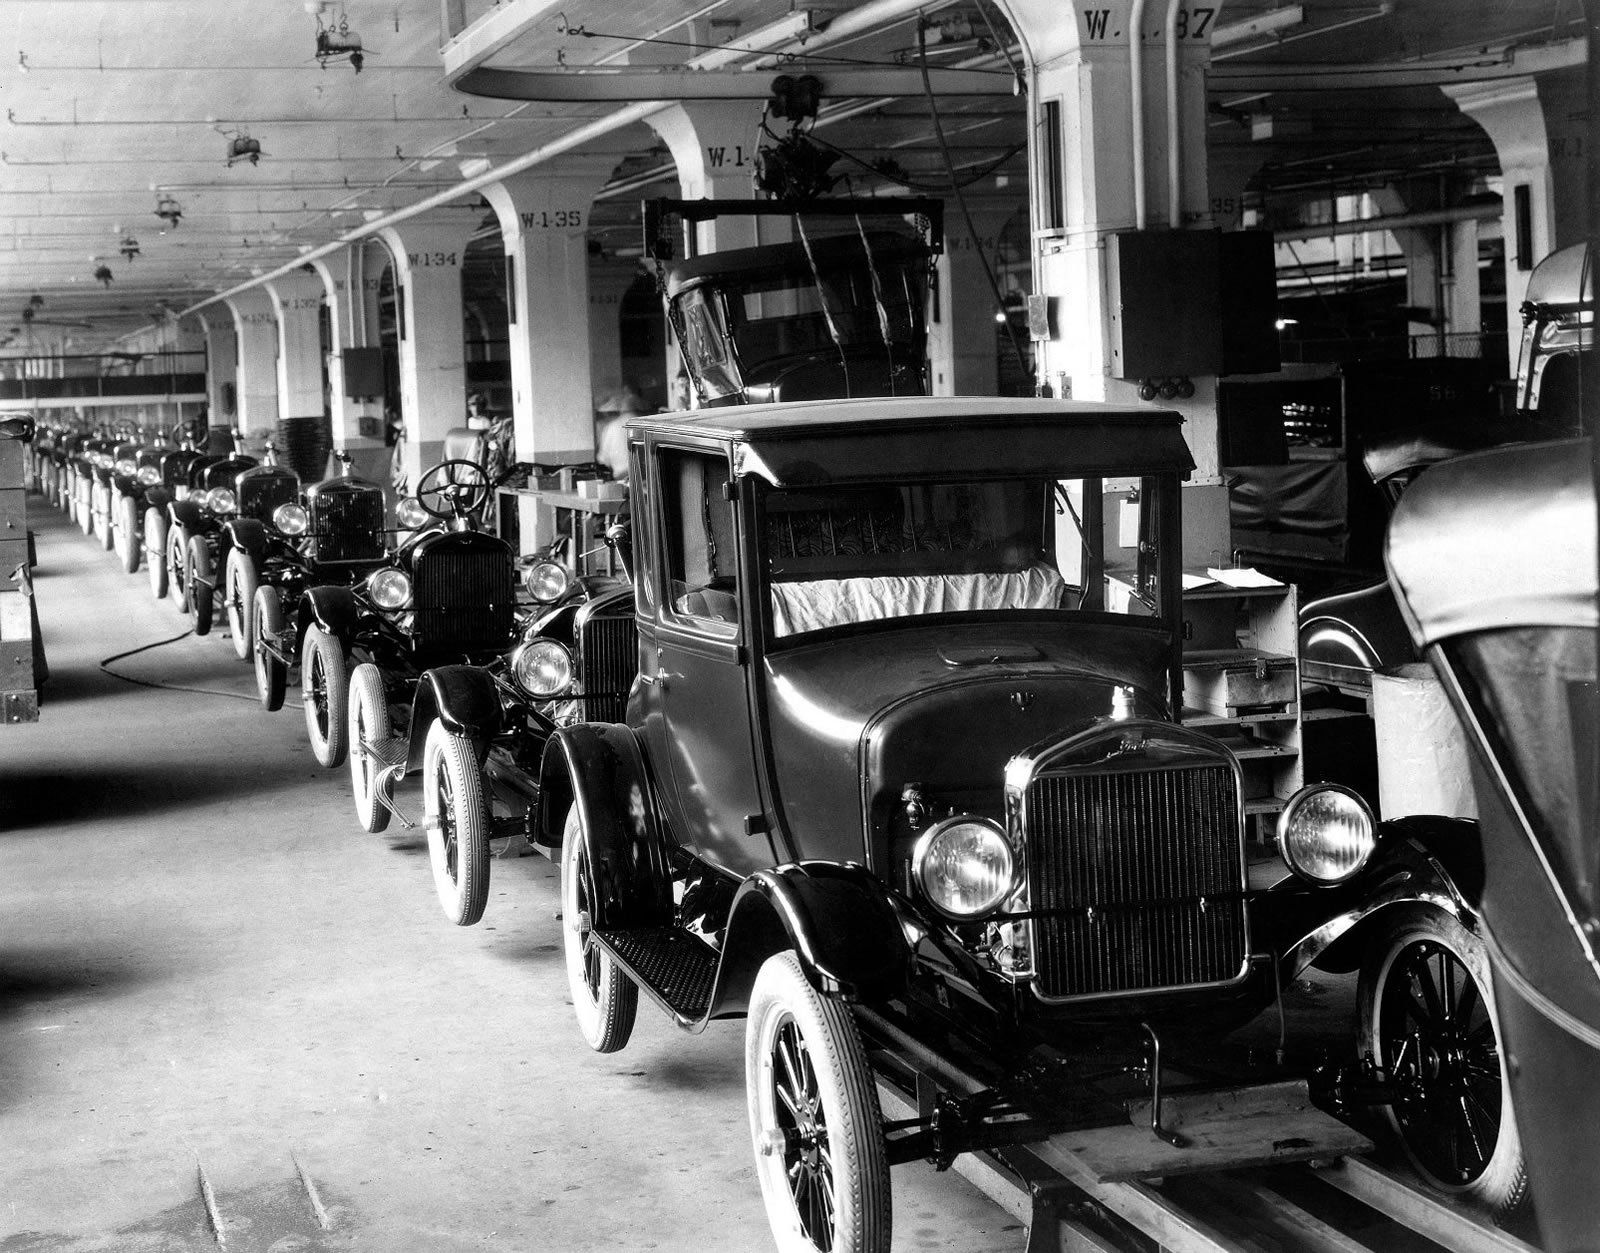
\includegraphics[width=.5 \textwidth]{figures/ford}
  \vfill\null
  \end{multicols}
\end{frame}


\begin{frame}{PS3, Ex. 6: Cournot Oligopoly with three firms}
  \begin{multicols}{2}
    \begin{itemize}
      \item[a)] Quantities in the Cournot equilibrium
    \end{itemize}
    The payoff function for firm $i\in\{1,2,3\}$:
    \begin{align*}
        \pi_i&=(1-q_i-q_j-q_k)q_i
    \end{align*}
  \vfill\null \columnbreak
  \vfill\null
  \end{multicols}
\end{frame}
\begin{frame}{PS3, Ex. 6: Cournot Oligopoly with three firms}
  \begin{multicols}{2}
    \begin{itemize}
      \item[a)] Quantities in the Cournot equilibrium
    \end{itemize}
    The payoff function for firm $i\in\{1,2,3\}$:
    \begin{align*}
        \pi_i&=(1-q_i-q_j-q_k)q_i
    \end{align*}
    Best-Response (BR) function for firm $i$:
    \begin{align*}
        \frac{\delta\pi_i}{\delta q_i}=1-2q_i-q_j-q_k&=0\\
                                                  q_i&=\frac{1-q_j-q_k}{2}
    \end{align*}
  \vfill\null \columnbreak
  \vfill\null
  \end{multicols}
\end{frame}
\begin{frame}{PS3, Ex. 6: Cournot Oligopoly with three firms}
  \begin{multicols}{2}
    \begin{itemize}
      \item[a)] Quantities in the Cournot equilibrium
    \end{itemize}
    The payoff function for firm $i\in\{1,2,3\}$:
    \begin{align*}
        \pi_i&=(1-q_i-q_j-q_k)q_i
    \end{align*}
    Best-Response (BR) function for firm $i$:
    \begin{align*}
        \frac{\delta\pi_i}{\delta q_i}=1-2q_i-q_j-q_k&=0\\
                                                  q_i&=\frac{1-q_j-q_k}{2}
    \end{align*}
    Due to symmetry $q_i^{*}=q_j^{*}=q_k^{*}=q^{NE}$:
    \begin{align*}
        q_i^{*} &= \frac{1-2q_i^{*}}{2}\\
        q_i^{*} &= \frac{1}{4}\equiv q^{NE}
    \end{align*}
  \vfill\null \columnbreak
  \vfill\null
  \end{multicols}
\end{frame}
\begin{frame}{PS3, Ex. 6: Cournot Oligopoly with three firms}
  \begin{multicols}{2}
    \begin{itemize}
      \item[a)] Quantities in the Cournot equilibrium
    \end{itemize}
    The payoff function for firm $i\in\{1,2,3\}$:
    \begin{align*}
        \pi_i&=(1-q_i-q_j-q_k)q_i
    \end{align*}
    Best-Response (BR) function for firm $i$:
    \begin{align*}
        \frac{\delta\pi_i}{\delta q_i}=1-2q_i-q_j-q_k&=0\\
                                                  q_i&=\frac{1-q_j-q_k}{2}
    \end{align*}
    Due to symmetry $q_i^{*}=q_j^{*}=q_k^{*}=q^{NE}$:
    \begin{align*}
        q_i^{*} &= \frac{1-2q_i^{*}}{2}\\
        q_i^{*} &= \frac{1}{4}\equiv q^{NE}
    \end{align*}
    \begin{itemize}
      \item[(b)] What is the price in the Cournot-equilibrium?
    \end{itemize}
  \vfill\null \columnbreak
  \vfill\null
  \end{multicols}
\end{frame}
\begin{frame}{PS3, Ex. 6: Cournot Oligopoly with three firms}
  \begin{multicols}{2}
    \begin{itemize}
      \item[a)] Quantities in the Cournot equilibrium
    \end{itemize}
    The payoff function for firm $i\in\{1,2,3\}$:
    \begin{align*}
        \pi_i&=(1-q_i-q_j-q_k)q_i
    \end{align*}
    Best-Response (BR) function for firm $i$:
    \begin{align*}
        \frac{\delta\pi_i}{\delta q_i}=1-2q_i-q_j-q_k&=0\\
                                                  q_i&=\frac{1-q_j-q_k}{2}
    \end{align*}
    Due to symmetry $q_i^{*}=q_j^{*}=q_k^{*}=q^{NE}$:
    \begin{align*}
        q_i^{*} &= \frac{1-2q_i^{*}}{2}\\
        q_i^{*} &= \frac{1}{4}\equiv q^{NE}
    \end{align*}
    \begin{itemize}
      \item[(b)] Price in the Cournot-equilibrium:
    \end{itemize}
    \begin{align*}
      p^{*}=1-q_i^{*}-q_j^{*}-q_k^{*}=\frac{1}{4}\Rightarrow\pi_i^{*}=\frac{1}{16}
    \end{align*}
  \vfill\null \columnbreak
  \vfill\null
  \end{multicols}
\end{frame}
\begin{frame}{PS3, Ex. 6: Cournot Oligopoly with three firms}
  \begin{multicols}{2}
    \begin{itemize}
      \item[a)] Quantities in the Cournot equilibrium
    \end{itemize}
    The payoff function for firm $i\in\{1,2,3\}$:
    \begin{align*}
        \pi_i&=(1-q_i-q_j-q_k)q_i
    \end{align*}
    Best-Response (BR) function for firm $i$:
    \begin{align*}
        \frac{\delta\pi_i}{\delta q_i}=1-2q_i-q_j-q_k&=0\\
                                                  q_i&=\frac{1-q_j-q_k}{2}
    \end{align*}
    Due to symmetry $q_i^{*}=q_j^{*}=q_k^{*}=q^{NE}$:
    \begin{align*}
        q_i^{*} &= \frac{1-2q_i^{*}}{2}\\
        q_i^{*} &= \frac{1}{4}\equiv q^{NE}
    \end{align*}
    \begin{itemize}
      \item[(b)] Price in the Cournot-equilibrium:
    \end{itemize}
    \begin{align*}
      p^{*}=1-q_i^{*}-q_j^{*}-q_k^{*}=\frac{1}{4}\Rightarrow\pi_i^{*}=\frac{1}{16}
    \end{align*}
  \vfill\null \columnbreak
    \begin{itemize}
      \item[(c)] Show that if two of the three firms merge (transforming the industry into a duopoly), the profits of the merging firms decrease. Explain.
    \end{itemize}
  \vfill\null
  \end{multicols}
\end{frame}
\begin{frame}{PS3, Ex. 6: Cournot Oligopoly with three firms}
  \begin{multicols}{2}
    \begin{itemize}
      \item[a)] Quantities in the Cournot equilibrium
    \end{itemize}
    The payoff function for firm $i\in\{1,2,3\}$:
    \begin{align*}
        \pi_i&=(1-q_i-q_j-q_k)q_i
    \end{align*}
    Best-Response (BR) function for firm $i$:
    \begin{align*}
        \frac{\delta\pi_i}{\delta q_i}=1-2q_i-q_j-q_k&=0\\
                                                  q_i&=\frac{1-q_j-q_k}{2}
    \end{align*}
    Due to symmetry $q_i^{*}=q_j^{*}=q_k^{*}=q^{NE}$:
    \begin{align*}
        q_i^{*} &= \frac{1-2q_i^{*}}{2}\\
        q_i^{*} &= \frac{1}{4}\equiv q^{NE}
    \end{align*}
    \begin{itemize}
      \item[(b)] Price in the Cournot-equilibrium:
    \end{itemize}
    \begin{align*}
      p^{*}=1-q_i^{*}-q_j^{*}-q_k^{*}=\frac{1}{4}\Rightarrow\pi_i^{*}=\frac{1}{16}
    \end{align*}
  \vfill\null \columnbreak
    \begin{itemize}
      \item[(c)] Firm \textit{1} and \textit{2} merge to firm $m$.
    \end{itemize}
    The payoff function for firm $i\in\{\bm{m},3\}$:
    \begin{align*}
        \pi_i&=(1-q_i-q_j)q_i
    \end{align*}
  \vfill\null
  \end{multicols}
\end{frame}
\begin{frame}{PS3, Ex. 6: Cournot Oligopoly with three firms}
  \begin{multicols}{2}
    \begin{itemize}
      \item[a)] Quantities in the Cournot equilibrium
    \end{itemize}
    The payoff function for firm $i\in\{1,2,3\}$:
    \begin{align*}
        \pi_i&=(1-q_i-q_j-q_k)q_i
    \end{align*}
    Best-Response (BR) function for firm $i$:
    \begin{align*}
        \frac{\delta\pi_i}{\delta q_i}=1-2q_i-q_j-q_k&=0\\
                                                  q_i&=\frac{1-q_j-q_k}{2}
    \end{align*}
    Due to symmetry $q_i^{*}=q_j^{*}=q_k^{*}=q^{NE}$:
    \begin{align*}
        q_i^{*} &= \frac{1-2q_i^{*}}{2}\\
        q_i^{*} &= \frac{1}{4}\equiv q^{NE}
    \end{align*}
    \begin{itemize}
      \item[(b)] Price in the Cournot-equilibrium:
    \end{itemize}
    \begin{align*}
      p^{*}=1-q_i^{*}-q_j^{*}-q_k^{*}=\frac{1}{4}\Rightarrow\pi_i^{*}=\frac{1}{16}
    \end{align*}
  \vfill\null \columnbreak
    \begin{itemize}
      \item[(c)] Firm \textit{1} and \textit{2} merge to firm $m$.
    \end{itemize}
    The payoff function for firm $i\in\{\bm{m},3\}$:
    \begin{align*}
        \pi_i&=(1-q_i-q_j)q_i
    \end{align*}
    BR function for firm $i$ in the duopoly:
    \begin{align*}
        q_i&=\frac{1-q_j}{2}\\
        q_i^{*} &= \frac{1-2q_i^{*}}{2},\ \ q_i^{*}=q_j^{*}\\
        q_i^{*} &= \frac{1}{3}\equiv q^{NE}
    \end{align*}
  \vfill\null
  \end{multicols}
\end{frame}
\begin{frame}{PS3, Ex. 6: Cournot Oligopoly with three firms}
  \begin{multicols}{2}
    \begin{itemize}
      \item[a)] Quantities in the Cournot equilibrium
    \end{itemize}
    The payoff function for firm $i\in\{1,2,3\}$:
    \begin{align*}
        \pi_i&=(1-q_i-q_j-q_k)q_i
    \end{align*}
    Best-Response (BR) function for firm $i$:
    \begin{align*}
        \frac{\delta\pi_i}{\delta q_i}=1-2q_i-q_j-q_k&=0\\
                                                  q_i&=\frac{1-q_j-q_k}{2}
    \end{align*}
    Due to symmetry $q_i^{*}=q_j^{*}=q_k^{*}=q^{NE}$:
    \begin{align*}
        q_i^{*} &= \frac{1-2q_i^{*}}{2}\\
        q_i^{*} &= \frac{1}{4}\equiv q^{NE}
    \end{align*}
    \begin{itemize}
      \item[(b)] Price in the Cournot-equilibrium:
    \end{itemize}
    \begin{align*}
      p^{*}=1-q_i^{*}-q_j^{*}-q_k^{*}=\frac{1}{4}\Rightarrow\pi_i^{*}=\frac{1}{16}
    \end{align*}
  \vfill\null \columnbreak
    \begin{itemize}
      \item[(c)] Firm \textit{1} and \textit{2} merge to firm $m$.
    \end{itemize}
    The payoff function for firm $i\in\{\bm{m},3\}$:
    \begin{align*}
        \pi_i&=(1-q_i-q_j)q_i
    \end{align*}
    BR function for firm $i$ in the duopoly:
    \begin{align*}
        q_i&=\frac{1-q_j}{2}\\
        q_i^{*} &= \frac{1-2q_i^{*}}{2},\ \ q_i^{*}=q_j^{*}\\
        q_i^{*} &= \frac{1}{3}\equiv q^{NE}
    \end{align*}
    By merging the rivalry is internalized by reducing joint output which increase market price and the profit margin:
    \begin{align*}
      p^{*}=1-q_m^{*}-q_3^{*}=\frac{1}{3}\Rightarrow\pi_m^{*}=\pi_3^{*}=\frac{1}{9}
    \end{align*}
    Are Firm \textit{1} and \textit{2} better or worse off? Why?
  \vfill\null
  \end{multicols}
\end{frame}
\begin{frame}{PS3, Ex. 6: Cournot Oligopoly with three firms}
  \begin{multicols}{2}
    \begin{itemize}
      \item[a)] Quantities in the Cournot equilibrium
    \end{itemize}
    The payoff function for firm $i\in\{1,2,3\}$:
    \begin{align*}
        \pi_i&=(1-q_i-q_j-q_k)q_i
    \end{align*}
    Best-Response (BR) function for firm $i$:
    \begin{align*}
        \frac{\delta\pi_i}{\delta q_i}=1-2q_i-q_j-q_k&=0\\
                                                  q_i&=\frac{1-q_j-q_k}{2}
    \end{align*}
    Due to symmetry $q_i^{*}=q_j^{*}=q_k^{*}=q^{NE}$:
    \begin{align*}
        q_i^{*} &= \frac{1-2q_i^{*}}{2}\\
        q_i^{*} &= \frac{1}{4}\equiv q^{NE}
    \end{align*}
    \begin{itemize}
      \item[(b)] Price in the Cournot-equilibrium:
    \end{itemize}
    \begin{align*}
      p^{*}=1-q_i^{*}-q_j^{*}-q_k^{*}=\frac{1}{4}\Rightarrow\pi_i^{*}=\frac{1}{16}
    \end{align*}
  \vfill\null \columnbreak
    \begin{itemize}
      \item[(c)] Firm \textit{1} and \textit{2} merge to firm $m$.
    \end{itemize}
    The payoff function for firm $i\in\{\bm{m},3\}$:
    \begin{align*}
        \pi_i&=(1-q_i-q_j)q_i
    \end{align*}
    BR function for firm $i$ in the duopoly:
    \begin{align*}
        q_i&=\frac{1-q_j}{2}\\
        q_i^{*} &= \frac{1-2q_i^{*}}{2},\ \ q_i^{*}=q_j^{*}\\
        q_i^{*} &= \frac{1}{3}\equiv q^{NE}
    \end{align*}
    By merging the rivalry is internalized by reducing joint output which increase market price and the profit margin:
    \begin{align*}
      p^{*}=1-q_m^{*}-q_3^{*}=\frac{1}{3}\Rightarrow\pi_m^{*}=\pi_3^{*}=\frac{1}{9}
    \end{align*}
    However, Firm \textit{1} and \textit{2} each get $\frac{1}{18}<\frac{1}{16}$ and are worse off as the third firm reacts to the higher price by increasing output.
  \vfill\null
  \end{multicols}
\end{frame}
\begin{frame}{PS3, Ex. 6: Cournot Oligopoly with three firms}
  \begin{multicols}{2}
    \begin{itemize}
      \item[a)] Quantities in the Cournot equilibrium
    \end{itemize}
    The payoff function for firm $i\in\{1,2,3\}$:
    \begin{align*}
        \pi_i&=(1-q_i-q_j-q_k)q_i
    \end{align*}
    Best-Response (BR) function for firm $i$:
    \begin{align*}
        \frac{\delta\pi_i}{\delta q_i}=1-2q_i-q_j-q_k&=0\\
                                                  q_i&=\frac{1-q_j-q_k}{2}
    \end{align*}
    Due to symmetry $q_i^{*}=q_j^{*}=q_k^{*}=q^{NE}$:
    \begin{align*}
        q_i^{*} &= \frac{1-2q_i^{*}}{2}\\
        q_i^{*} &= \frac{1}{4}\equiv q^{NE}
    \end{align*}
    \begin{itemize}
      \item[(b)] Price in the Cournot-equilibrium:
    \end{itemize}
    \begin{align*}
      p^{*}=1-q_i^{*}-q_j^{*}-q_k^{*}=\frac{1}{4}\Rightarrow\pi_i^{*}=\frac{1}{16}
    \end{align*}
  \vfill\null \columnbreak
    \begin{itemize}
      \item[(c)] Firm \textit{1} and \textit{2} merge to firm $m$.
    \end{itemize}
    \begin{align*}
        \pi_i&=(1-q_i-q_j)q_i
    \end{align*}
    \begin{align*}
        q_i^{*} &= \frac{1}{3}\equiv q^{NE}
    \end{align*}
    By merging the rivalry is internalized by reducing joint output which increase market price and the profit margin:
    \begin{align*}
      p^{*}=1-q_m^{*}-q_3^{*}=\frac{1}{3}\Rightarrow\pi_m^{*}=\pi_3^{*}=\frac{1}{9}
    \end{align*}
    However, Firm \textit{1} and \textit{2} each get $\frac{1}{18}<\frac{1}{16}$ and are worse off as the third firm reacts to the higher price by increasing output.
    \begin{itemize}
      \item[(d)] What happens if all three firms merge?
    \end{itemize}
  \vfill\null
  \end{multicols}
\end{frame}
\begin{frame}{PS3, Ex. 6: Cournot Oligopoly with three firms}
  \begin{multicols}{2}
    \begin{itemize}
      \item[a)] Quantities in the Cournot equilibrium
    \end{itemize}
    The payoff function for firm $i\in\{1,2,3\}$:
    \begin{align*}
        \pi_i&=(1-q_i-q_j-q_k)q_i
    \end{align*}
    Best-Response (BR) function for firm $i$:
    \begin{align*}
        \frac{\delta\pi_i}{\delta q_i}=1-2q_i-q_j-q_k&=0\\
                                                  q_i&=\frac{1-q_j-q_k}{2}
    \end{align*}
    Due to symmetry $q_i^{*}=q_j^{*}=q_k^{*}=q^{NE}$:
    \begin{align*}
        q_i^{*} &= \frac{1-2q_i^{*}}{2}\\
        q_i^{*} &= \frac{1}{4}\equiv q^{NE}
    \end{align*}
    \begin{itemize}
      \item[(b)] Price in the Cournot-equilibrium:
    \end{itemize}
    \begin{align*}
      p^{*}=1-q_i^{*}-q_j^{*}-q_k^{*}=\frac{1}{4}\Rightarrow\pi_i^{*}=\frac{1}{16}
    \end{align*}
  \vfill\null \columnbreak
    \begin{itemize}
      \item[(c)] Firm \textit{1} and \textit{2} merge to firm $m$.
    \end{itemize}
    \begin{align*}
        \pi_i&=(1-q_i-q_j)q_i
    \end{align*}
    \begin{align*}
        q_i^{*} &= \frac{1}{3}\equiv q^{NE}
    \end{align*}
    By merging the rivalry is internalized by reducing joint output which increase market price and the profit margin:
    \begin{align*}
      p^{*}=1-q_m^{*}-q_3^{*}=\frac{1}{3}\Rightarrow\pi_m^{*}=\pi_3^{*}=\frac{1}{9}
    \end{align*}
    However, Firm \textit{1} and \textit{2} each get $\frac{1}{18}<\frac{1}{16}$ and are worse off as the third firm reacts to the higher price by increasing output.
    \begin{itemize}
      \item[(d)] A full merger maximizes joint profits:
    \end{itemize}
    \begin{align*}
      q_\text{monopoly}^{*}=p_\text{monopoly}^{*}=\frac{1}{2}\Rightarrow \pi_\text{monopoly}^{*}=\frac{1}{4}>\frac{2}{9}
    \end{align*}
  \vfill\null
  \end{multicols}
\end{frame}



\section{PS3, Ex. 7: Mixed Strategy Nash Equilibria - (p,q)-diagrams}

\begin{frame}{PS3, Ex. 7: Mixed Strategy Nash Equilibria - (p,q)-diagrams}
  Plot the mixed best responses of each player (in a "(p,q)-diagram" - see the textbook). And find all Nash equilibria (pure and mixed) in the games below
  \begin{multicols}{2}
    \begin{itemize}
      \item[(a)]
    \end{itemize}
    \vspace{-16pt}
    \begin{table}
      \begin{tabular}{cl|c|c|}
          & \multicolumn{1}{c}{} & \multicolumn{2}{c}{Player 2}\\
          \parbox[t]{1mm}{\multirow{3}{*}{\rotatebox[origin=r]{90}{Player 1}}}
          & \multicolumn{1}{c}{} & \multicolumn{1}{c}{L ($q$)} & \multicolumn{1}{c}{R (1-$q$)} \\\cline{3-4}
          & T  ($p$)  & 0, 0 & 0, 0 \\\cline{3-4}
          & B  (1-$p$)& 0, 0 & 1, 1 \\\cline{3-4}
      \end{tabular}
    \end{table}
    \begin{itemize}
      \item[(b)]
    \end{itemize}
    \vspace{-16pt}
    \begin{table}
      \begin{tabular}{cl|c|c|}
          & \multicolumn{1}{c}{} & \multicolumn{2}{c}{Player 2}\\
          \parbox[t]{1mm}{\multirow{3}{*}{\rotatebox[origin=r]{90}{Player 1}}}
          & \multicolumn{1}{c}{} & \multicolumn{1}{c}{L ($q$)} & \multicolumn{1}{c}{R (1-$q$)} \\\cline{3-4}
          & T  ($p$)  & 1, 3 & 1, 0 \\\cline{3-4}
          & B  (1-$p$)& 1, 1 & 5, 5 \\\cline{3-4}
      \end{tabular}
    \end{table}
  \vfill\null \columnbreak
  \begin{itemize}
    \item[(c)]
  \end{itemize}
  \vspace{-16pt}
  \begin{table}
    \begin{tabular}{cl|c|c|}
        & \multicolumn{1}{c}{} & \multicolumn{2}{c}{Player 2}\\
        \parbox[t]{1mm}{\multirow{3}{*}{\rotatebox[origin=r]{90}{Player 1}}}
        & \multicolumn{1}{c}{} & \multicolumn{1}{c}{L ($q$)} & \multicolumn{1}{c}{R (1-$q$)} \\\cline{3-4}
        & T  ($p$)  & 3, 2 & 1, 2 \\\cline{3-4}
        & B  (1-$p$)& 0, 1 & 1, 2 \\\cline{3-4}
    \end{tabular}
  \end{table}
  \begin{itemize}
    \item[(d)]
  \end{itemize}
  \vspace{-16pt}
  \begin{table}
    \begin{tabular}{cl|c|c|}
        & \multicolumn{1}{c}{} & \multicolumn{2}{c}{Player 2}\\
        & \multicolumn{1}{c}{} & \multicolumn{1}{c}{$t_1$ ($q$)} & \multicolumn{1}{c}{$t_2$ (1-$q$)} \\\cline{3-4}
        \parbox[t]{1mm}{\multirow{3}{*}{\rotatebox[origin=c]{90}{Player 1}}}
        & $s_1$ ($p_1$)         & 2, 1 & 3, 0 \\\cline{3-4}
        & $s_2$ ($p_2$)         & 1, 2 & 4, 3 \\\cline{3-4}
        & $s_3$ (1-$p_1$-$p_2$) & 0, 1 & 0, 3 \\\cline{3-4}
    \end{tabular}
  \end{table}
  \vfill\null
  \end{multicols}
\end{frame}
\begin{frame}{PS3, Ex. 7: Mixed Strategy Nash Equilibria - (p,q)-diagrams}
  Plot the mixed best responses of each player (in a "(p,q)-diagram" - see the textbook). And find all Nash equilibria (pure and mixed) in the games below
  \begin{multicols}{2}
    \begin{itemize}
      \item[(a)]
    \end{itemize}
    \vspace{-16pt}
    \begin{table}
      \begin{tabular}{cl|c|c|}
          & \multicolumn{1}{c}{} & \multicolumn{2}{c}{Player 2}\\
          \parbox[t]{1mm}{\multirow{3}{*}{\rotatebox[origin=r]{90}{Player 1}}}
          & \multicolumn{1}{c}{} & \multicolumn{1}{c}{L ($q$)} & \multicolumn{1}{c}{R (1-$q$)} \\\cline{3-4}
          & T  ($p$)  & 0, 0 & 0, 0 \\\cline{3-4}
          & B  (1-$p$)& 0, 0 & 1, 1 \\\cline{3-4}
      \end{tabular}
    \end{table}
    \begin{itemize}
      \item[(b)]
    \end{itemize}
    \vspace{-16pt}
    \begin{table}
      \begin{tabular}{cl|c|c|}
          & \multicolumn{1}{c}{} & \multicolumn{2}{c}{Player 2}\\
          \parbox[t]{1mm}{\multirow{3}{*}{\rotatebox[origin=r]{90}{Player 1}}}
          & \multicolumn{1}{c}{} & \multicolumn{1}{c}{L ($q$)} & \multicolumn{1}{c}{R (1-$q$)} \\\cline{3-4}
          & T  ($p$)  & 1, 3 & 1, 0 \\\cline{3-4}
          & B  (1-$p$)& 1, 1 & 5, 5 \\\cline{3-4}
      \end{tabular}
    \end{table}
  \vfill\null \columnbreak
  \begin{itemize}
    \item[(c)]
  \end{itemize}
  \vspace{-16pt}
  \begin{table}
    \begin{tabular}{cl|c|c|}
        & \multicolumn{1}{c}{} & \multicolumn{2}{c}{Player 2}\\
        \parbox[t]{1mm}{\multirow{3}{*}{\rotatebox[origin=r]{90}{Player 1}}}
        & \multicolumn{1}{c}{} & \multicolumn{1}{c}{L ($q$)} & \multicolumn{1}{c}{R (1-$q$)} \\\cline{3-4}
        & T  ($p$)  & 3, 2 & 1, 2 \\\cline{3-4}
        & B  (1-$p$)& 0, 1 & 1, 2 \\\cline{3-4}
    \end{tabular}
  \end{table}
  \begin{itemize}
    \item[(d)]
  \end{itemize}
  \vspace{-16pt}
  \begin{table}
    \begin{tabular}{cl|c|c|}
        & \multicolumn{1}{c}{} & \multicolumn{2}{c}{Player 2}\\
        & \multicolumn{1}{c}{} & \multicolumn{1}{c}{$t_1$ ($q$)} & \multicolumn{1}{c}{$t_2$ (1-$q$)} \\\cline{3-4}
        \parbox[t]{1mm}{\multirow{3}{*}{\rotatebox[origin=c]{90}{Player 1}}}
        & $s_1$ ($p_1$)         & 2, 1 & 3, 0 \\\cline{3-4}
        & $s_2$ ($p_2$)         & 1, 2 & 4, 3 \\\cline{3-4}
        & $s_3$ (1-$p_1$-$p_2$) & 0, 1 & 0, 3 \\\cline{3-4}
    \end{tabular}
  \end{table}
  \vfill\null
  \end{multicols}
  \begin{tabular}{|l|}
      \cline{1-1}
      \textbf{Hint}: Find the probabilities $q$ for which Player 1 is indifferent, e.g. $u_1(T,q)=u_1(B,q)$.\\
                      and the probabilities $p$ for which Player 2 is indifferent, e.g. $u_2(L,p)=u_2(R,p)$.\\\cline{1-1}
  \end{tabular}
\end{frame}

\begin{frame}{PS3, Ex. 7.a: Mixed Strategy Nash Equilibria - (p,q)-diagrams}
  \begin{multicols}{2}
    \begin{itemize}
      \item[(a)] Plot the mixed best responses and find all NE (pure and mixed):
    \end{itemize}
    \vspace{-10pt}
    \begin{table}
      \begin{tabular}{cl|c|c|}
        & \multicolumn{1}{c}{} & \multicolumn{2}{c}{\color{blue}Player 2}\\
        \parbox[t]{1mm}{\multirow{3}{*}{\rotatebox[origin=r]{90}{\color{red}Player 1}}}
          & \multicolumn{1}{c}{} & \multicolumn{1}{c}{L ($q$)} & \multicolumn{1}{c}{R (1-$q$)} \\\cline{3-4}
          & T  ($p$)  & \textcolor{red}{0}, \textcolor{blue}{0} & 0, \textcolor{blue}{0} \\\cline{3-4}
          & B  (1-$p$)& \textcolor{red}{0}, 0 & \textcolor{red}{1}, \textcolor{blue}{1} \\\cline{3-4}
      \end{tabular}
    \end{table}
  \vfill\null \columnbreak
    \textit{For which values of $q$ is Player 1 indifferent?}
  \vfill\null
  \end{multicols}
\end{frame}
\begin{frame}{PS3, Ex. 7.a: Mixed Strategy Nash Equilibria - (p,q)-diagrams}
  \begin{multicols}{2}
    \begin{itemize}
      \item[(a)] Plot the mixed best responses and find all NE (pure and mixed):
    \end{itemize}
    \vspace{-10pt}
    \begin{table}
      \begin{tabular}{cl|c|c|}
        & \multicolumn{1}{c}{} & \multicolumn{2}{c}{\color{blue}Player 2}\\
        \parbox[t]{1mm}{\multirow{3}{*}{\rotatebox[origin=r]{90}{\color{red}Player 1}}}
          & \multicolumn{1}{c}{} & \multicolumn{1}{c}{L ($q$)} & \multicolumn{1}{c}{R (1-$q$)} \\\cline{3-4}
          & T  ($p$)  & \textcolor{red}{0}, \textcolor{blue}{0} & 0, \textcolor{blue}{0} \\\cline{3-4}
          & B  (1-$p$)& \textcolor{red}{0}, 0 & \textcolor{red}{1}, \textcolor{blue}{1} \\\cline{3-4}
      \end{tabular}
    \end{table}
    Player 1:
    \begin{itemize}
      \item Indifferent if $q=1\Rightarrow p\in[0,1]$
      \item Prefers $B$ if $q<1\Rightarrow p=0$.
    \end{itemize}
  \vfill\null \columnbreak
    \textit{Write up Player 1's best-response (BR) function, $p^{*}(q)$.}
  \vfill\null
  \end{multicols}
\end{frame}
\begin{frame}{PS3, Ex. 7.a: Mixed Strategy Nash Equilibria - (p,q)-diagrams}
  \begin{multicols}{2}
    \begin{itemize}
      \item[(a)] Plot the mixed best responses and find all NE (pure and mixed):
    \end{itemize}
    \vspace{-10pt}
    \begin{table}
      \begin{tabular}{cl|c|c|}
        & \multicolumn{1}{c}{} & \multicolumn{2}{c}{\color{blue}Player 2}\\
        \parbox[t]{1mm}{\multirow{3}{*}{\rotatebox[origin=r]{90}{\color{red}Player 1}}}
          & \multicolumn{1}{c}{} & \multicolumn{1}{c}{L ($q$)} & \multicolumn{1}{c}{R (1-$q$)} \\\cline{3-4}
          & T  ($p$)  & \textcolor{red}{0}, \textcolor{blue}{0} & 0, \textcolor{blue}{0} \\\cline{3-4}
          & B  (1-$p$)& \textcolor{red}{0}, 0 & \textcolor{red}{1}, \textcolor{blue}{1} \\\cline{3-4}
      \end{tabular}
    \end{table}
    Player 1:
    \begin{itemize}
      \item Indifferent if $q=1\Rightarrow p\in[0,1]$
      \item Prefers $B$ if $q<1\Rightarrow p=0$.
    \end{itemize}
    Player 1's BR function, $p^{*}(q)$:
    \begin{align*}
      BR_1(q)=\left\{ \begin{array}{lcl}
      p=0       & \text{if} & q<1 \\
      p\in[0,1] & \text{if} & q=1
      \end{array}\right.
    \end{align*}
  \vfill\null \columnbreak
    \textit{Plot Player 1's BR function, $p^{*}(q)$, in a (p,q)-diagram.}
  \vfill\null
  \end{multicols}
\end{frame}
\begin{frame}{PS3, Ex. 7.a: Mixed Strategy Nash Equilibria - (p,q)-diagrams}
  \begin{multicols}{2}
    \begin{itemize}
      \item[(a)] Plot the mixed best responses and find all NE (pure and mixed):
    \end{itemize}
    \vspace{-10pt}
    \begin{table}
      \begin{tabular}{cl|c|c|}
        & \multicolumn{1}{c}{} & \multicolumn{2}{c}{\color{blue}Player 2}\\
        \parbox[t]{1mm}{\multirow{3}{*}{\rotatebox[origin=r]{90}{\color{red}Player 1}}}
          & \multicolumn{1}{c}{} & \multicolumn{1}{c}{L ($q$)} & \multicolumn{1}{c}{R (1-$q$)} \\\cline{3-4}
          & T  ($p$)  & \textcolor{red}{0}, \textcolor{blue}{0} & 0, \textcolor{blue}{0} \\\cline{3-4}
          & B  (1-$p$)& \textcolor{red}{0}, 0 & \textcolor{red}{1}, \textcolor{blue}{1} \\\cline{3-4}
      \end{tabular}
    \end{table}
    Player 1:
    \begin{itemize}
      \item Indifferent if $q=1\Rightarrow p\in[0,1]$
      \item Prefers $B$ if $q<1\Rightarrow p=0$.
    \end{itemize}
    Player 1's BR function, $p^{*}(q)$:
    \begin{align*}
      BR_1(q)=\left\{ \begin{array}{lcl}
      p=0       & \text{if} & q<1 \\
      p\in[0,1] & \text{if} & q=1
      \end{array}\right.
    \end{align*}
  \vfill\null \columnbreak
    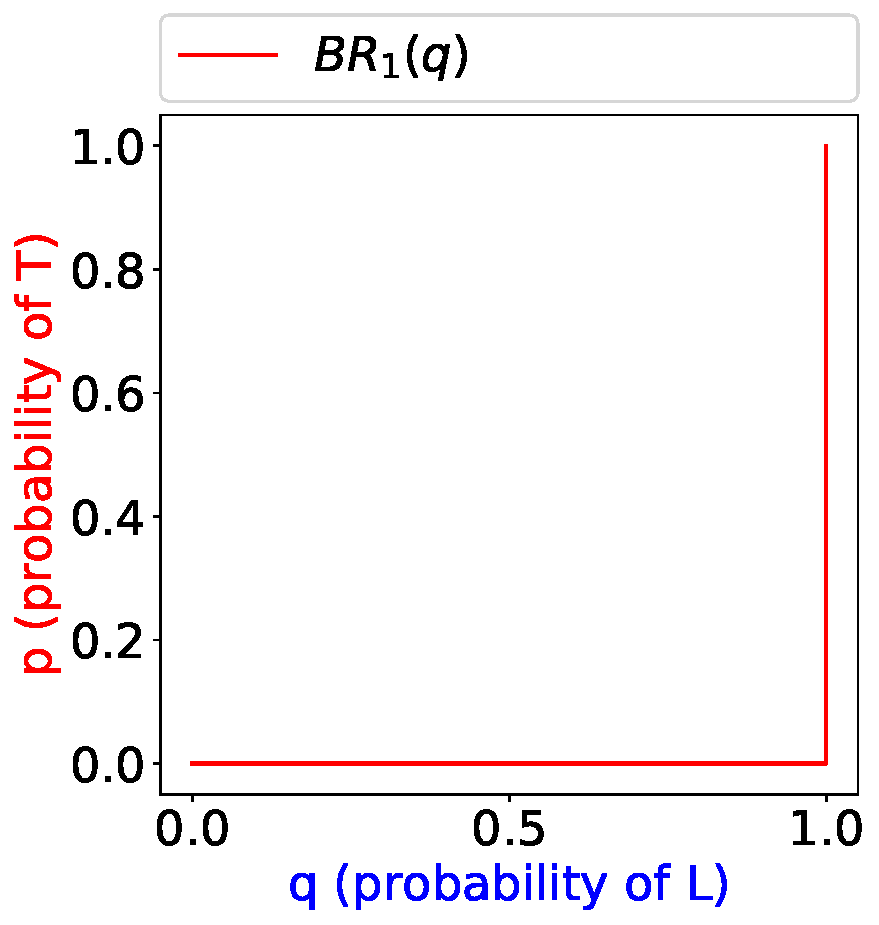
\includegraphics[width=\columnwidth]{figures/7a1}
    \textit{For which values of $p$ is Player 2 indifferent?}
  \vfill\null
  \end{multicols}
\end{frame}
\begin{frame}{PS3, Ex. 7.a: Mixed Strategy Nash Equilibria - (p,q)-diagrams}
  \begin{multicols}{2}
    \begin{itemize}
      \item[(a)] Plot the mixed best responses and find all NE (pure and mixed):
    \end{itemize}
    \vspace{-10pt}
    \begin{table}
      \begin{tabular}{cl|c|c|}
        & \multicolumn{1}{c}{} & \multicolumn{2}{c}{\color{blue}Player 2}\\
        \parbox[t]{1mm}{\multirow{3}{*}{\rotatebox[origin=r]{90}{\color{red}Player 1}}}
          & \multicolumn{1}{c}{} & \multicolumn{1}{c}{L ($q$)} & \multicolumn{1}{c}{R (1-$q$)} \\\cline{3-4}
          & T  ($p$)  & \textcolor{red}{0}, \textcolor{blue}{0} & 0, \textcolor{blue}{0} \\\cline{3-4}
          & B  (1-$p$)& \textcolor{red}{0}, 0 & \textcolor{red}{1}, \textcolor{blue}{1} \\\cline{3-4}
      \end{tabular}
    \end{table}
    Player 1:
    \begin{itemize}
      \item Indifferent if $q=1\Rightarrow p\in[0,1]$
      \item Prefers $B$ if $q<1\Rightarrow p=0$.
    \end{itemize}
    \begin{align*}
      BR_1(q)=\left\{ \begin{array}{lcl}
      p=0       & \text{if} & q<1 \\
      p\in[0,1] & \text{if} & q=1
      \end{array}\right.
    \end{align*}
    Player 2:
    \begin{itemize}
      \item Indifferent if $p=1\Rightarrow q\in[0,1]$
      \item Prefers $R$ if $p<1\Rightarrow q=0$.
    \end{itemize}
  \vfill\null \columnbreak
    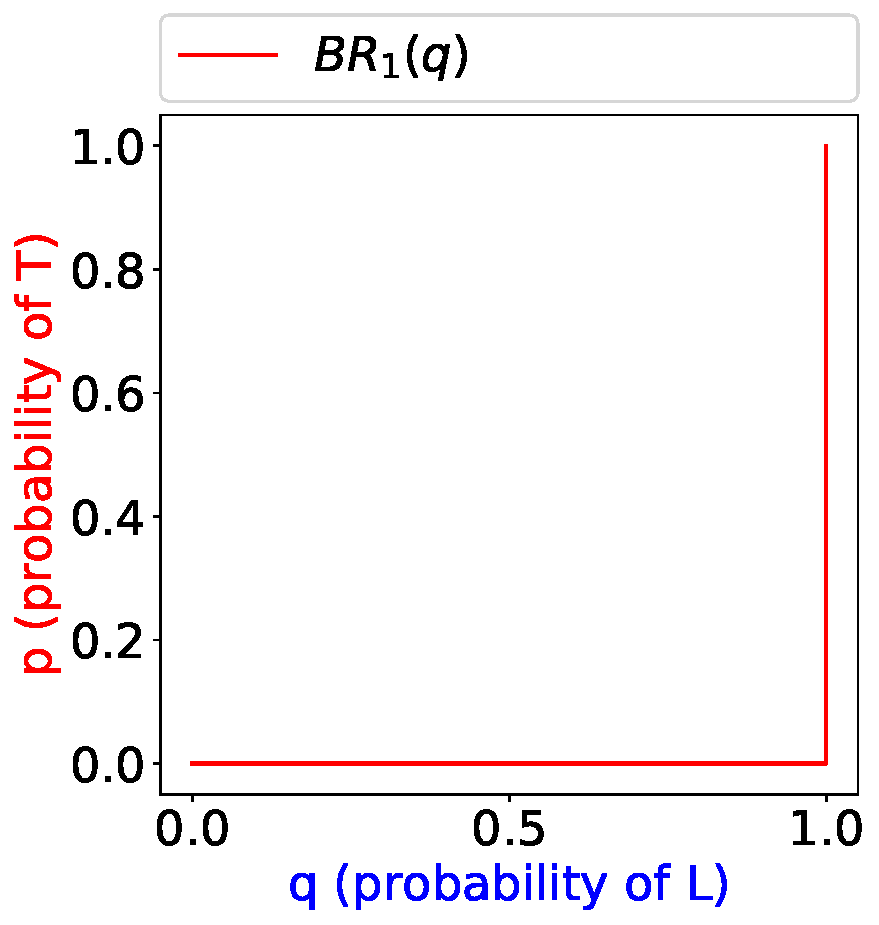
\includegraphics[width=\columnwidth]{figures/7a1}
    \textit{Write up Player 2's best-response (BR) function, $q^{*}(p)$}
  \vfill\null
  \end{multicols}
\end{frame}
\begin{frame}{PS3, Ex. 7.a: Mixed Strategy Nash Equilibria - (p,q)-diagrams}
  \begin{multicols}{2}
    \begin{itemize}
      \item[(a)] Plot the mixed best responses and find all NE (pure and mixed):
    \end{itemize}
    \vspace{-10pt}
    \begin{table}
      \begin{tabular}{cl|c|c|}
        & \multicolumn{1}{c}{} & \multicolumn{2}{c}{\color{blue}Player 2}\\
        \parbox[t]{1mm}{\multirow{3}{*}{\rotatebox[origin=r]{90}{\color{red}Player 1}}}
          & \multicolumn{1}{c}{} & \multicolumn{1}{c}{L ($q$)} & \multicolumn{1}{c}{R (1-$q$)} \\\cline{3-4}
          & T  ($p$)  & \textcolor{red}{0}, \textcolor{blue}{0} & 0, \textcolor{blue}{0} \\\cline{3-4}
          & B  (1-$p$)& \textcolor{red}{0}, 0 & \textcolor{red}{1}, \textcolor{blue}{1} \\\cline{3-4}
      \end{tabular}
    \end{table}
    Player 1:
    \begin{itemize}
      \item Indifferent if $q=1\Rightarrow p\in[0,1]$
      \item Prefers $B$ if $q<1\Rightarrow p=0$.
    \end{itemize}
    \begin{align*}
      BR_1(q)=\left\{ \begin{array}{lcl}
      p=0       & \text{if} & q<1 \\
      p\in[0,1] & \text{if} & q=1
      \end{array}\right.
    \end{align*}
    Player 2:
    \begin{itemize}
      \item Indifferent if $p=1\Rightarrow q\in[0,1]$
      \item Prefers $R$ if $p<1\Rightarrow q=0$.
    \end{itemize}
    Player 2's BR function, $q^{*}(p)$:
    \begin{align*}
      BR_2(p)=\left\{ \begin{array}{lcl}
      q=0       & \text{if} & p<1  \\
      q\in[0,1] & \text{if} & p=1
      \end{array}\right.
    \end{align*}
  \vfill\null \columnbreak
    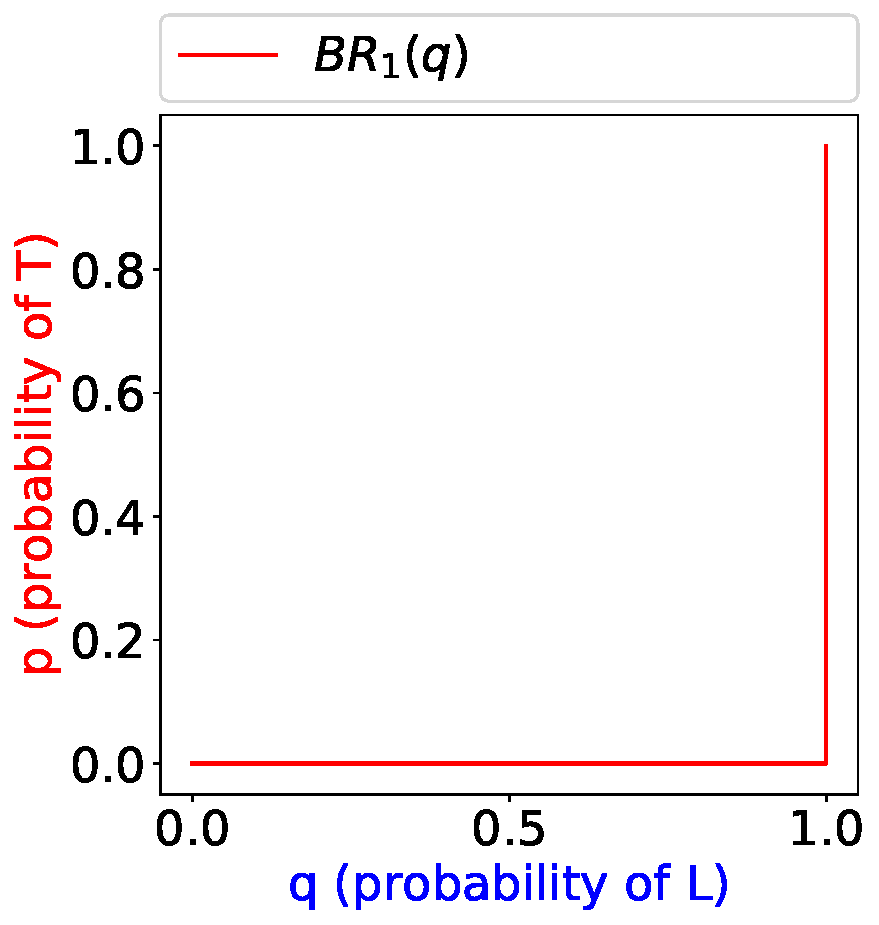
\includegraphics[width=\columnwidth]{figures/7a1}
    \textit{Plot Player 2's BR function, $q^{*}(p)$}
  \vfill\null
  \end{multicols}
\end{frame}
\begin{frame}{PS3, Ex. 7.a: Mixed Strategy Nash Equilibria - (p,q)-diagrams}
  \begin{multicols}{2}
    \begin{itemize}
      \item[(a)] Plot the mixed best responses and find all NE (pure and mixed):
    \end{itemize}
    \vspace{-10pt}
    \begin{table}
      \begin{tabular}{cl|c|c|}
        & \multicolumn{1}{c}{} & \multicolumn{2}{c}{\color{blue}Player 2}\\
        \parbox[t]{1mm}{\multirow{3}{*}{\rotatebox[origin=r]{90}{\color{red}Player 1}}}
          & \multicolumn{1}{c}{} & \multicolumn{1}{c}{L ($q$)} & \multicolumn{1}{c}{R (1-$q$)} \\\cline{3-4}
          & T  ($p$)  & \textcolor{red}{0}, \textcolor{blue}{0} & 0, \textcolor{blue}{0} \\\cline{3-4}
          & B  (1-$p$)& \textcolor{red}{0}, 0 & \textcolor{red}{1}, \textcolor{blue}{1} \\\cline{3-4}
      \end{tabular}
    \end{table}
    Player 1:
    \begin{itemize}
      \item Indifferent if $q=1\Rightarrow p\in[0,1]$
      \item Prefers $B$ if $q<1\Rightarrow p=0$.
    \end{itemize}
    \begin{align*}
      BR_1(q)=\left\{ \begin{array}{lcl}
      p=0       & \text{if} & q<1 \\
      p\in[0,1] & \text{if} & q=1
      \end{array}\right.
    \end{align*}
    Player 2:
    \begin{itemize}
      \item Indifferent if $p=1\Rightarrow q\in[0,1]$
      \item Prefers $R$ if $p<1\Rightarrow q=0$.
    \end{itemize}
    \begin{align*}
      BR_2(p)=\left\{ \begin{array}{lcl}
      q=0       & \text{if} & p<1  \\
      q\in[0,1] & \text{if} & p=1
      \end{array}\right.
    \end{align*}
  \vfill\null \columnbreak
    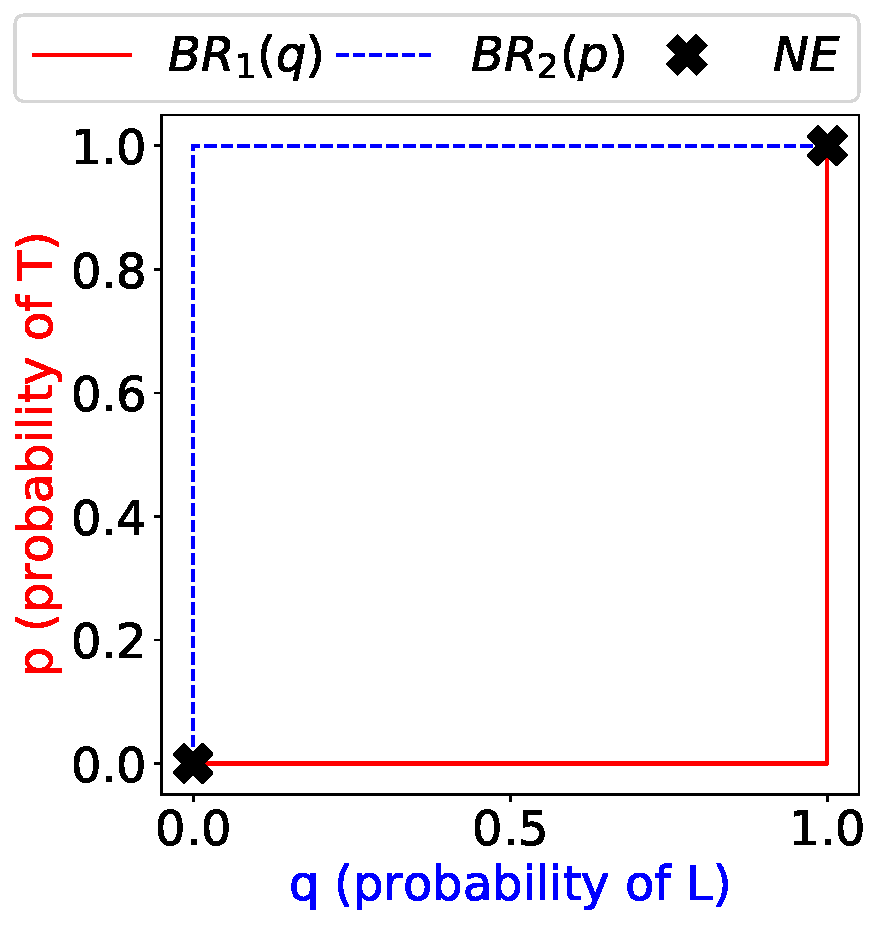
\includegraphics[width=\columnwidth]{figures/7a2}
    \textit{Write up all NE (pure and mixed).}
  \vfill\null
  \end{multicols}
\end{frame}
\begin{frame}{PS3, Ex. 7.a: Mixed Strategy Nash Equilibria - (p,q)-diagrams}
  \begin{multicols}{2}
    \begin{itemize}
      \item[(a)] Plot the mixed best responses and find all NE (pure and mixed):
    \end{itemize}
    \vspace{-10pt}
    \begin{table}
      \begin{tabular}{cl|c|c|}
        & \multicolumn{1}{c}{} & \multicolumn{2}{c}{\color{blue}Player 2}\\
        \parbox[t]{1mm}{\multirow{3}{*}{\rotatebox[origin=r]{90}{\color{red}Player 1}}}
          & \multicolumn{1}{c}{} & \multicolumn{1}{c}{L ($q$)} & \multicolumn{1}{c}{R (1-$q$)} \\\cline{3-4}
          & T  ($p$)  & \textcolor{red}{0}, \textcolor{blue}{0} & 0, \textcolor{blue}{0} \\\cline{3-4}
          & B  (1-$p$)& \textcolor{red}{0}, 0 & \textcolor{red}{1}, \textcolor{blue}{1} \\\cline{3-4}
      \end{tabular}
    \end{table}
    Player 1:
    \begin{itemize}
      \item Indifferent if $q=1\Rightarrow p\in[0,1]$
      \item Prefers $B$ if $q<1\Rightarrow p=0$.
    \end{itemize}
    \begin{align*}
      BR_1(q)=\left\{ \begin{array}{lcl}
      p=0       & \text{if} & q<1 \\
      p\in[0,1] & \text{if} & q=1
      \end{array}\right.
    \end{align*}
    Player 2:
    \begin{itemize}
      \item Indifferent if $p=1\Rightarrow q\in[0,1]$
      \item Prefers $R$ if $p<1\Rightarrow q=0$.
    \end{itemize}
    \begin{align*}
      BR_2(p)=\left\{ \begin{array}{lcl}
      q=0       & \text{if} & p<1  \\
      q\in[0,1] & \text{if} & p=1
      \end{array}\right.
    \end{align*}
  \vfill\null \columnbreak
    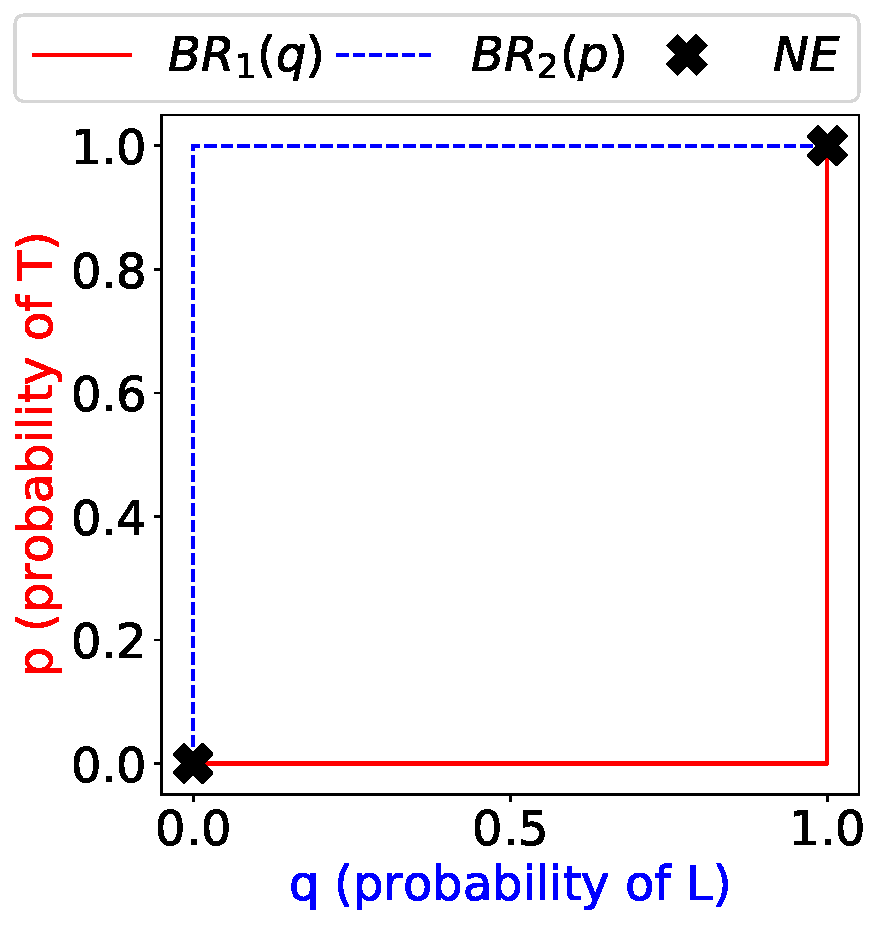
\includegraphics[width=\columnwidth]{figures/7a2}
    Two Pure Strategy Nash Equilibria:
    \begin{align*}
      PSNE=\{(T,L),(B,R)\}
    \end{align*}
    We find two Mixed Strategy NE (MSNE). Both coincide with the PSNE:
    \begin{align*}
      (p^{*},q^{*})=\left\{(1,1),(0,0)\right\}
    \end{align*}  \vfill\null
  \end{multicols}
\end{frame}

\begin{frame}{PS3, Ex. 7.b: Mixed Strategy Nash Equilibria - (p,q)-diagrams}
  \begin{multicols}{2}
    \begin{itemize}
      \item[(b)] Plot the mixed best responses and find all NE (pure and mixed):
    \end{itemize}
    \vspace{-10pt}
    \begin{table}
      \begin{tabular}{cl|c|c|}
        & \multicolumn{1}{c}{} & \multicolumn{2}{c}{\color{blue}Player 2}\\
        \parbox[t]{1mm}{\multirow{3}{*}{\rotatebox[origin=r]{90}{\color{red}Player 1}}}
        & \multicolumn{1}{c}{} & \multicolumn{1}{c}{L ($q$)} & \multicolumn{1}{c}{R (1-$q$)} \\\cline{3-4}
        & T  ($p$)  & \textcolor{red}{1}, \textcolor{blue}{3} & 1, 0 \\\cline{3-4}
        & B  (1-$p$)& \textcolor{red}{1}, 1 & \textcolor{red}{5}, \textcolor{blue}{5} \\\cline{3-4}
      \end{tabular}
    \end{table}
  \vfill\null \columnbreak
    \textit{For which values of $q$ is Player 1 indifferent?}
  \vfill\null
  \end{multicols}
\end{frame}
\begin{frame}{PS3, Ex. 7.b: Mixed Strategy Nash Equilibria - (p,q)-diagrams}
  \begin{multicols}{2}
    \begin{itemize}
      \item[(b)] Plot the mixed best responses and find all NE (pure and mixed):
    \end{itemize}
    \begin{table}
      \begin{tabular}{cl|c|c|}
        & \multicolumn{1}{c}{} & \multicolumn{2}{c}{\color{blue}Player 2}\\
        \parbox[t]{1mm}{\multirow{3}{*}{\rotatebox[origin=r]{90}{\color{red}Player 1}}}
        & \multicolumn{1}{c}{} & \multicolumn{1}{c}{L ($q$)} & \multicolumn{1}{c}{R (1-$q$)} \\\cline{3-4}
        & T  ($p$)  & \textcolor{red}{1}, \textcolor{blue}{3} & 1, 0 \\\cline{3-4}
        & B  (1-$p$)& \textcolor{red}{1}, 1 & \textcolor{red}{5}, \textcolor{blue}{5} \\\cline{3-4}
      \end{tabular}
    \end{table}
    Player 1 is indifferent if:
    \begin{align*}
      1 &= 1q + 5(1-q) \\
      5q&= 4 \Rightarrow q = 1
    \end{align*}
  \vfill\null \columnbreak
  \textit{Write up Player 1's best-response (BR) function, $p^{*}(q)$.}
  \vfill\null
  \end{multicols}
\end{frame}
\begin{frame}{PS3, Ex. 7.b: Mixed Strategy Nash Equilibria - (p,q)-diagrams}
  \begin{multicols}{2}
    \begin{itemize}
      \item[(b)] Plot the mixed best responses and find all NE (pure and mixed):
    \end{itemize}
    \vspace{-10pt}
    \begin{table}
      \begin{tabular}{cl|c|c|}
        & \multicolumn{1}{c}{} & \multicolumn{2}{c}{\color{blue}Player 2}\\
        \parbox[t]{1mm}{\multirow{3}{*}{\rotatebox[origin=r]{90}{\color{red}Player 1}}}
        & \multicolumn{1}{c}{} & \multicolumn{1}{c}{L ($q$)} & \multicolumn{1}{c}{R (1-$q$)} \\\cline{3-4}
        & T  ($p$)  & \textcolor{red}{1}, \textcolor{blue}{3} & 1, 0 \\\cline{3-4}
        & B  (1-$p$)& \textcolor{red}{1}, 1 & \textcolor{red}{5}, \textcolor{blue}{5} \\\cline{3-4}
      \end{tabular}
    \end{table}
    Player 1 is indifferent if:
    \begin{align*}
      1 &= 1q + 5(1-q) \\
      5q&= 4 \Rightarrow q = 1
    \end{align*}
    Player 1's BR function, $p^{*}(q)$:
    \begin{align*}
      BR_1(q)=\left\{ \begin{array}{lcl}
      p=0       & \text{if} & q<1 \\
      p\in[0,1] & \text{if} & q=1
      \end{array}\right.
    \end{align*}
  \vfill\null \columnbreak
    \textit{Plot Player 1's BR function, $p^{*}(q)$, in a (p,q)-diagram.}
  \vfill\null
  \end{multicols}
\end{frame}
\begin{frame}{PS3, Ex. 7.b: Mixed Strategy Nash Equilibria - (p,q)-diagrams}
  \begin{multicols}{2}
    \begin{itemize}
      \item[(b)] Plot the mixed best responses and find all NE (pure and mixed):
    \end{itemize}
    \vspace{-10pt}
    \begin{table}
      \begin{tabular}{cl|c|c|}
        & \multicolumn{1}{c}{} & \multicolumn{2}{c}{\color{blue}Player 2}\\
        \parbox[t]{1mm}{\multirow{3}{*}{\rotatebox[origin=r]{90}{\color{red}Player 1}}}
        & \multicolumn{1}{c}{} & \multicolumn{1}{c}{L ($q$)} & \multicolumn{1}{c}{R (1-$q$)} \\\cline{3-4}
        & T  ($p$)  & \textcolor{red}{1}, \textcolor{blue}{3} & 1, 0 \\\cline{3-4}
        & B  (1-$p$)& \textcolor{red}{1}, 1 & \textcolor{red}{5}, \textcolor{blue}{5} \\\cline{3-4}
      \end{tabular}
    \end{table}
    Player 1 is indifferent if:
    \begin{align*}
      1 &= 1q + 5(1-q) \\
      5q&= 4 \Rightarrow q = 1
    \end{align*}
    Player 1's BR function, $p^{*}(q)$:
    \begin{align*}
      BR_1(q)=\left\{ \begin{array}{lcl}
      p=0       & \text{if} & q<1 \\
      p\in[0,1] & \text{if} & q=1
      \end{array}\right.
    \end{align*}
  \vfill\null \columnbreak
    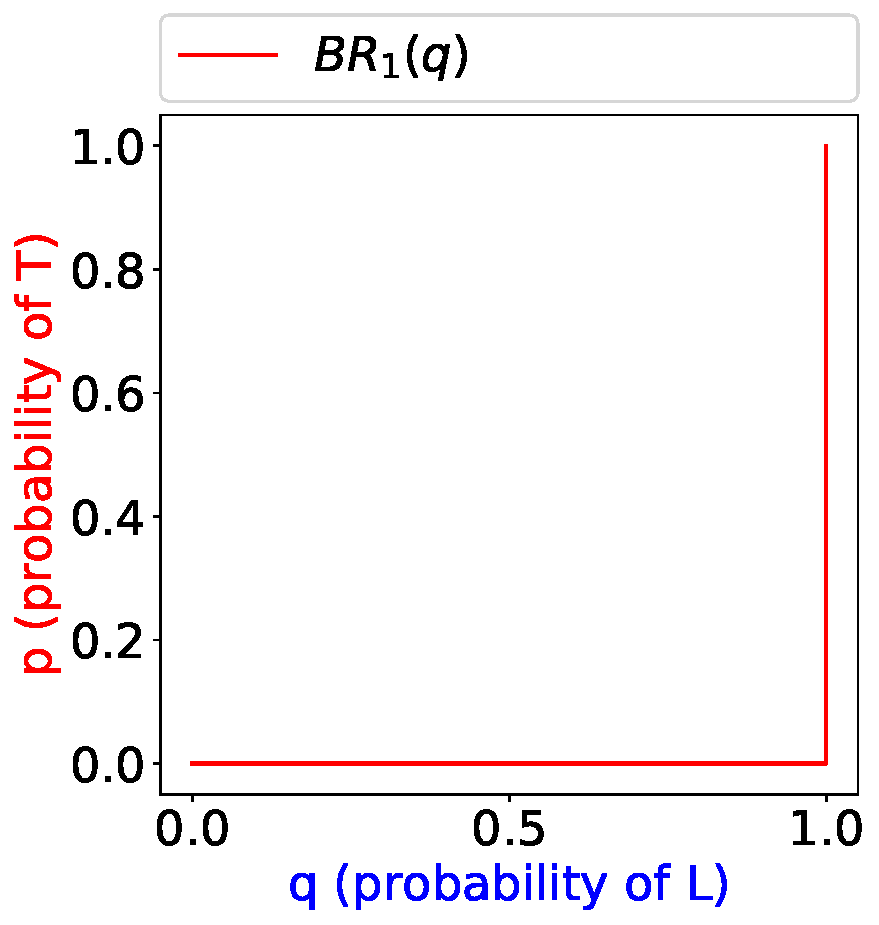
\includegraphics[width=\columnwidth]{figures/7b1}
    \textit{For which values of $p$ is Player 2 indifferent?}
  \vfill\null
  \end{multicols}
\end{frame}
\begin{frame}{PS3, Ex. 7.b: Mixed Strategy Nash Equilibria - (p,q)-diagrams}
  \begin{multicols}{2}
    \begin{itemize}
      \item[(b)] Plot the mixed best responses and find all NE (pure and mixed):
    \end{itemize}
    \vspace{-10pt}
    \begin{table}
      \begin{tabular}{cl|c|c|}
        & \multicolumn{1}{c}{} & \multicolumn{2}{c}{\color{blue}Player 2}\\
        \parbox[t]{1mm}{\multirow{3}{*}{\rotatebox[origin=r]{90}{\color{red}Player 1}}}
        & \multicolumn{1}{c}{} & \multicolumn{1}{c}{L ($q$)} & \multicolumn{1}{c}{R (1-$q$)} \\\cline{3-4}
        & T  ($p$)  & \textcolor{red}{1}, \textcolor{blue}{3} & 1, 0 \\\cline{3-4}
        & B  (1-$p$)& \textcolor{red}{1}, 1 & \textcolor{red}{5}, \textcolor{blue}{5} \\\cline{3-4}
      \end{tabular}
    \end{table}
    Player 1 is indifferent if:
    \begin{align*}
      1 &= 1q + 5(1-q) \\
      5q&= 4 \Rightarrow q = 1
    \end{align*}
    \begin{align*}
      BR_1(q)=\left\{ \begin{array}{lcl}
      p=0       & \text{if} & q<1 \\
      p\in[0,1] & \text{if} & q=1
      \end{array}\right.
    \end{align*}
    Player 2 is indifferent if:
    \begin{align*}
      3p + 1(1-p)&= 0p+5(1-p)\\
      7p         &= 4 \Rightarrow p = \frac{4}{7}
    \end{align*}
  \vfill\null \columnbreak
    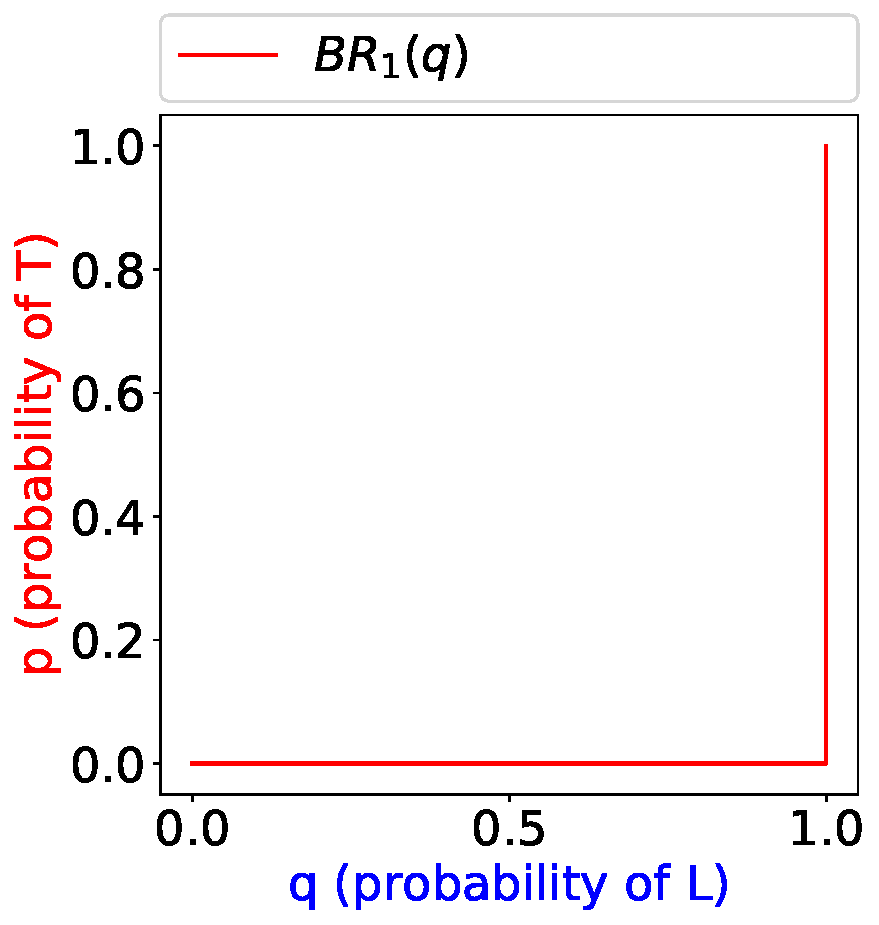
\includegraphics[width=\columnwidth]{figures/7b1}
    \textit{Write up Player 2's best-response (BR) function, $q^{*}(p)$}
  \vfill\null
  \end{multicols}
\end{frame}
\begin{frame}{PS3, Ex. 7.b: Mixed Strategy Nash Equilibria - (p,q)-diagrams}
  \begin{multicols}{2}
    \begin{itemize}
      \item[(b)] Plot the mixed best responses and find all NE (pure and mixed):
    \end{itemize}
    \vspace{-10pt}
    \begin{table}
      \begin{tabular}{cl|c|c|}
        & \multicolumn{1}{c}{} & \multicolumn{2}{c}{\color{blue}Player 2}\\
        \parbox[t]{1mm}{\multirow{3}{*}{\rotatebox[origin=r]{90}{\color{red}Player 1}}}
        & \multicolumn{1}{c}{} & \multicolumn{1}{c}{L ($q$)} & \multicolumn{1}{c}{R (1-$q$)} \\\cline{3-4}
        & T  ($p$)  & \textcolor{red}{1}, \textcolor{blue}{3} & 1, 0 \\\cline{3-4}
        & B  (1-$p$)& \textcolor{red}{1}, 1 & \textcolor{red}{5}, \textcolor{blue}{5} \\\cline{3-4}
      \end{tabular}
    \end{table}
    Player 1 is indifferent if:
    \begin{align*}
      1 &= 1q + 5(1-q) \\
      5q&= 4 \Rightarrow q = 1
    \end{align*}
    \begin{align*}
      BR_1(q)=\left\{ \begin{array}{lcl}
      p=0       & \text{if} & q<1 \\
      p\in[0,1] & \text{if} & q=1
      \end{array}\right.
    \end{align*}
    Player 2 is indifferent if:
    \begin{align*}
      3p + 1(1-p)&= 0p+5(1-p)\\
      7p         &= 4 \Rightarrow p = \frac{4}{7}
    \end{align*}
    \begin{align*}
      BR_2(p)=\left\{ \begin{array}{lcl}
      q=0       & \text{if} & p<4/7 \\
      q\in[0,1] & \text{if} & p=4/7 \\
      q=1       & \text{if} & p<4/7
      \end{array}\right.
    \end{align*}
  \vfill\null \columnbreak
    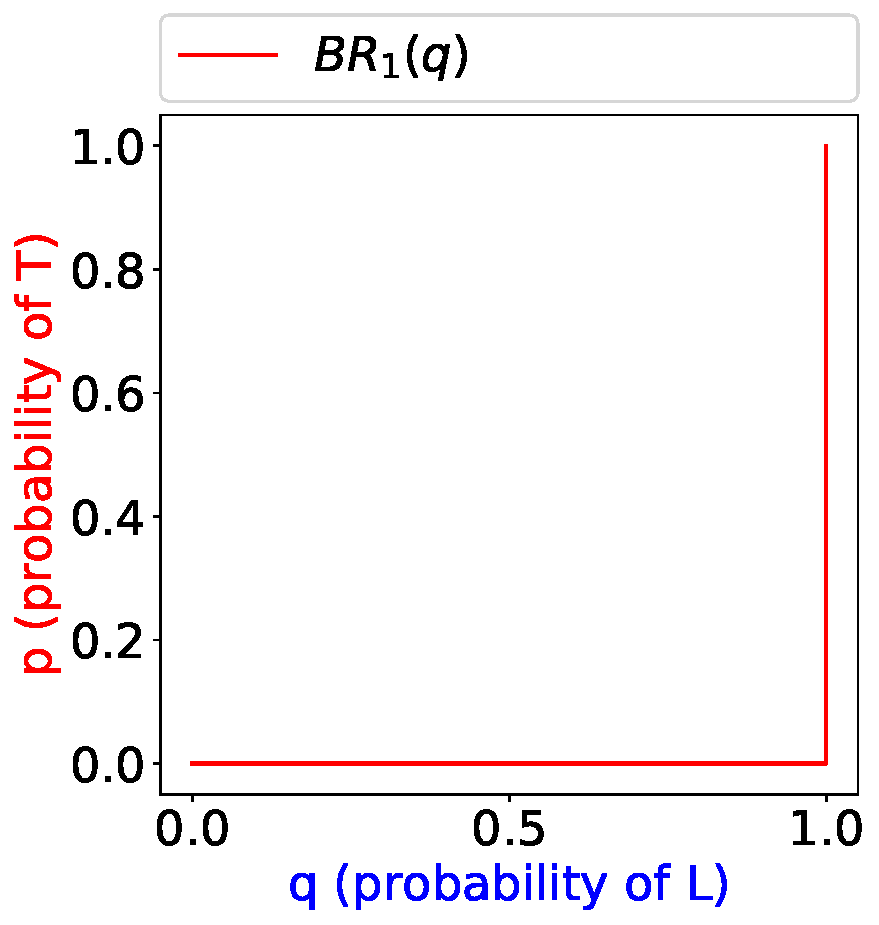
\includegraphics[width=\columnwidth]{figures/7b1}
    \textit{Plot Player 2's BR function, $q^{*}(p)$}
  \vfill\null
  \end{multicols}
\end{frame}
\begin{frame}{PS3, Ex. 7.b: Mixed Strategy Nash Equilibria - (p,q)-diagrams}
  \begin{multicols}{2}
    \begin{itemize}
      \item[(b)] Plot the mixed best responses and find all NE (pure and mixed):
    \end{itemize}
    \vspace{-10pt}
    \begin{table}
      \begin{tabular}{cl|c|c|}
        & \multicolumn{1}{c}{} & \multicolumn{2}{c}{\color{blue}Player 2}\\
        \parbox[t]{1mm}{\multirow{3}{*}{\rotatebox[origin=r]{90}{\color{red}Player 1}}}
        & \multicolumn{1}{c}{} & \multicolumn{1}{c}{L ($q$)} & \multicolumn{1}{c}{R (1-$q$)} \\\cline{3-4}
        & T  ($p$)  & \textcolor{red}{1}, \textcolor{blue}{3} & 1, 0 \\\cline{3-4}
        & B  (1-$p$)& \textcolor{red}{1}, 1 & \textcolor{red}{5}, \textcolor{blue}{5} \\\cline{3-4}
      \end{tabular}
    \end{table}
    Player 1 is indifferent if:
    \begin{align*}
      1 &= 1q + 5(1-q) \\
      5q&= 4 \Rightarrow q = 1
    \end{align*}
    \begin{align*}
      BR_1(q)=\left\{ \begin{array}{lcl}
      p=0       & \text{if} & q<1 \\
      p\in[0,1] & \text{if} & q=1
      \end{array}\right.
    \end{align*}
    Player 2 is indifferent if:
    \begin{align*}
      3p + 1(1-p)&= 0p+5(1-p)\\
      7p         &= 4 \Rightarrow p = \frac{4}{7}
    \end{align*}
    \begin{align*}
      BR_2(p)=\left\{ \begin{array}{lcl}
      q=0       & \text{if} & p<4/7 \\
      q\in[0,1] & \text{if} & p=4/7 \\
      q=1       & \text{if} & p<4/7
      \end{array}\right.
    \end{align*}
  \vfill\null \columnbreak
    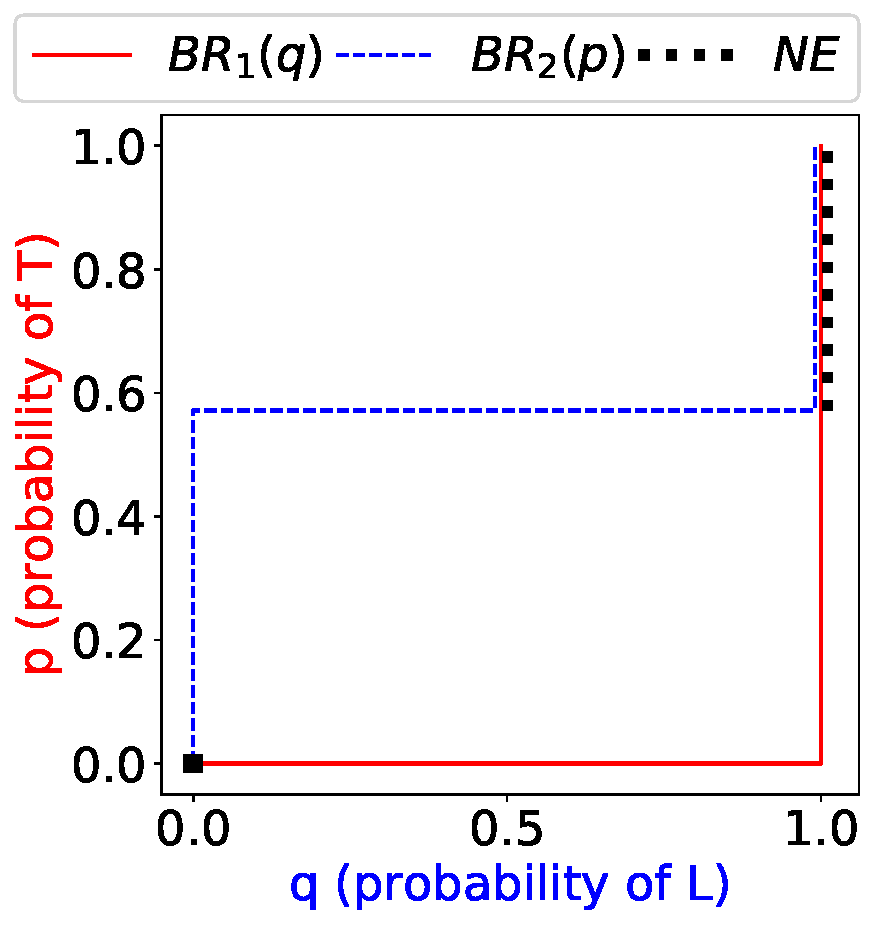
\includegraphics[width=\columnwidth]{figures/7b2}
    \textit{Write up all NE (pure and mixed).}
  \vfill\null
  \end{multicols}
\end{frame}
\begin{frame}{PS3, Ex. 7.b: Mixed Strategy Nash Equilibria - (p,q)-diagrams}
  \begin{multicols}{2}
    \begin{itemize}
      \item[(b)] Plot the mixed best responses and find all NE (pure and mixed):
    \end{itemize}
    \vspace{-10pt}
    \begin{table}
      \begin{tabular}{cl|c|c|}
        & \multicolumn{1}{c}{} & \multicolumn{2}{c}{\color{blue}Player 2}\\
        \parbox[t]{1mm}{\multirow{3}{*}{\rotatebox[origin=r]{90}{\color{red}Player 1}}}
        & \multicolumn{1}{c}{} & \multicolumn{1}{c}{L ($q$)} & \multicolumn{1}{c}{R (1-$q$)} \\\cline{3-4}
        & T  ($p$)  & \textcolor{red}{1}, \textcolor{blue}{3} & 1, 0 \\\cline{3-4}
        & B  (1-$p$)& \textcolor{red}{1}, 1 & \textcolor{red}{5}, \textcolor{blue}{5} \\\cline{3-4}
      \end{tabular}
    \end{table}
    Player 1 is indifferent if:
    \begin{align*}
      1 &= 1q + 5(1-q) \\
      5q&= 4 \Leftrightarrow q = 1
    \end{align*}
    \begin{align*}
      BR_1(q)=\left\{ \begin{array}{lcl}
      p=0       & \text{if} & q<1 \\
      p\in[0,1] & \text{if} & q=1
      \end{array}\right.
    \end{align*}
    Player 2 is indifferent if:
    \begin{align*}
      3p + 1(1-p)&= 0p+5(1-p)\\
      7p         &= 4 \Leftrightarrow p = \frac{4}{7}
    \end{align*}
    \vspace{-8pt}
    \begin{align*}
      BR_2(p)=\left\{ \begin{array}{lcl}
      q=0       & \text{if} & p<4/7 \\
      q\in[0,1] & \text{if} & p=4/7 \\
      q=1       & \text{if} & p<4/7
      \end{array}\right.
    \end{align*}
  \vfill\null \columnbreak
    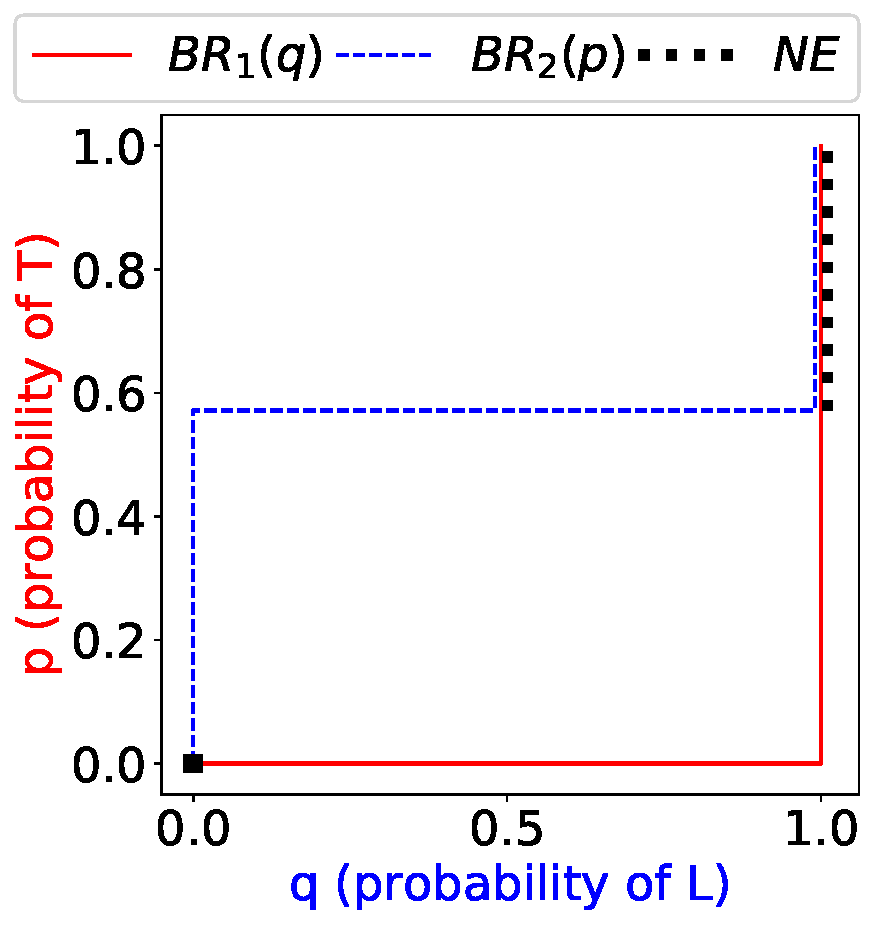
\includegraphics[width=\columnwidth]{figures/7b2}
    The pure and mixed strategy NE are:
    \begin{align*}
      (p^{*},q^{*})=\left\{(0,0);(1,1);\left(p\in\left[\frac{4}{7},1\right),q=1\right)\right\}
    \end{align*}
  \vfill\null
  \end{multicols}
\end{frame}

\begin{frame}{PS3, Ex. 7.c: Mixed Strategy Nash Equilibria - (p,q)-diagrams}
  \begin{multicols}{2}
    \begin{itemize}
      \item[(c)] Plot the mixed best responses and find all NE (pure and mixed):
    \end{itemize}
    \vspace{-10pt}
    \begin{table}
      \begin{tabular}{cl|c|c|}
        & \multicolumn{1}{c}{} & \multicolumn{2}{c}{\color{blue}Player 2}\\
        \parbox[t]{1mm}{\multirow{3}{*}{\rotatebox[origin=r]{90}{\color{red}Player 1}}}
        & \multicolumn{1}{c}{} & \multicolumn{1}{c}{L ($q$)} & \multicolumn{1}{c}{R (1-$q$)} \\\cline{3-4}
        & T  ($p$)  & \textcolor{red}{3}, \textcolor{blue}{2} & \textcolor{red}{1}, \textcolor{blue}{2} \\\cline{3-4}
        & B  (1-$p$)& 0, 1 & \textcolor{red}{1}, \textcolor{blue}{2} \\\cline{3-4}
      \end{tabular}
    \end{table}
  \vfill\null \columnbreak
    \textit{For which values of $q$ is Player 1 indifferent?}
  \vfill\null
  \end{multicols}
\end{frame}
\begin{frame}{PS3, Ex. 7.c: Mixed Strategy Nash Equilibria - (p,q)-diagrams}
  \begin{multicols}{2}
    \begin{itemize}
      \item[(c)] Plot the mixed best responses and find all NE (pure and mixed):
    \end{itemize}
    \vspace{-10pt}
    \begin{table}
      \begin{tabular}{cl|c|c|}
        & \multicolumn{1}{c}{} & \multicolumn{2}{c}{\color{blue}Player 2}\\
        \parbox[t]{1mm}{\multirow{3}{*}{\rotatebox[origin=r]{90}{\color{red}Player 1}}}
        & \multicolumn{1}{c}{} & \multicolumn{1}{c}{L ($q$)} & \multicolumn{1}{c}{R (1-$q$)} \\\cline{3-4}
        & T  ($p$)  & \textcolor{red}{3}, \textcolor{blue}{2} & \textcolor{red}{1}, \textcolor{blue}{2} \\\cline{3-4}
        & B  (1-$p$)& 0, 1 & \textcolor{red}{1}, \textcolor{blue}{2} \\\cline{3-4}
      \end{tabular}
    \end{table}
    Player 1 is indifferent if:
    \begin{align*}
      3q+(1-q) &= (1-q) \\
      q &= 0
    \end{align*}
  \vfill\null \columnbreak
    \textit{Write up Player 1's best-response (BR) function, $p^{*}(q)$.}
  \vfill\null
  \end{multicols}
\end{frame}
\begin{frame}{PS3, Ex. 7.c: Mixed Strategy Nash Equilibria - (p,q)-diagrams}
  \begin{multicols}{2}
    \begin{itemize}
      \item[(c)] Plot the mixed best responses and find all NE (pure and mixed):
    \end{itemize}
    \vspace{-10pt}
    \begin{table}
      \begin{tabular}{cl|c|c|}
        & \multicolumn{1}{c}{} & \multicolumn{2}{c}{\color{blue}Player 2}\\
        \parbox[t]{1mm}{\multirow{3}{*}{\rotatebox[origin=r]{90}{\color{red}Player 1}}}
        & \multicolumn{1}{c}{} & \multicolumn{1}{c}{L ($q$)} & \multicolumn{1}{c}{R (1-$q$)} \\\cline{3-4}
        & T  ($p$)  & \textcolor{red}{3}, \textcolor{blue}{2} & \textcolor{red}{1}, \textcolor{blue}{2} \\\cline{3-4}
        & B  (1-$p$)& 0, 1 & \textcolor{red}{1}, \textcolor{blue}{2} \\\cline{3-4}
      \end{tabular}
    \end{table}
    Player 1 is indifferent if:
    \begin{align*}
      3q+(1-q) &= (1-q) \\
      q &= 0
    \end{align*}
    Player 1's BR function, $p^{*}(q)$:
    \begin{align*}
      BR_1(q)=\left\{ \begin{array}{lcl}
      p\in[0,1] & \text{if} & q=0 \\
      p=1       & \text{if} & q>0
      \end{array}\right.
    \end{align*}
  \vfill\null \columnbreak
    \textit{Plot Player 1's BR function, $p^{*}(q)$, in a (p,q)-diagram.}
  \vfill\null
  \end{multicols}
\end{frame}
\begin{frame}{PS3, Ex. 7.c: Mixed Strategy Nash Equilibria - (p,q)-diagrams}
  \begin{multicols}{2}
    \begin{itemize}
      \item[(c)] Plot the mixed best responses and find all NE (pure and mixed):
    \end{itemize}
    \vspace{-10pt}
    \begin{table}
      \begin{tabular}{cl|c|c|}
        & \multicolumn{1}{c}{} & \multicolumn{2}{c}{\color{blue}Player 2}\\
        \parbox[t]{1mm}{\multirow{3}{*}{\rotatebox[origin=r]{90}{\color{red}Player 1}}}
        & \multicolumn{1}{c}{} & \multicolumn{1}{c}{L ($q$)} & \multicolumn{1}{c}{R (1-$q$)} \\\cline{3-4}
        & T  ($p$)  & \textcolor{red}{3}, \textcolor{blue}{2} & \textcolor{red}{1}, \textcolor{blue}{2} \\\cline{3-4}
        & B  (1-$p$)& 0, 1 & \textcolor{red}{1}, \textcolor{blue}{2} \\\cline{3-4}
      \end{tabular}
    \end{table}
    Player 1 is indifferent if:
    \begin{align*}
      3q+(1-q) &= (1-q) \\
      q &= 0
    \end{align*}
    Player 1's BR function, $p^{*}(q)$:
    \begin{align*}
      BR_1(q)=\left\{ \begin{array}{lcl}
      p\in[0,1] & \text{if} & q=0 \\
      p=1       & \text{if} & q>0
      \end{array}\right.
    \end{align*}
  \vfill\null \columnbreak
    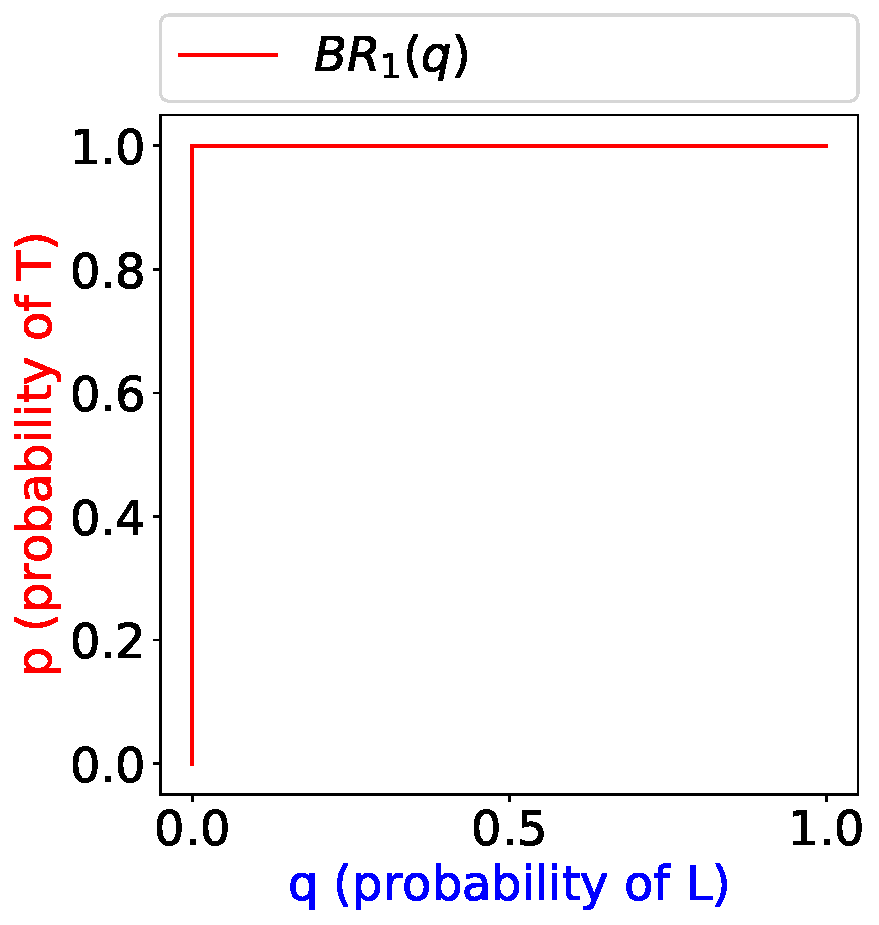
\includegraphics[width=\columnwidth]{figures/7c1}
    \textit{For which values of $p$ is Player 2 indifferent?}
  \vfill\null
  \end{multicols}
\end{frame}
\begin{frame}{PS3, Ex. 7.c: Mixed Strategy Nash Equilibria - (p,q)-diagrams}
  \begin{multicols}{2}
    \begin{itemize}
      \item[(c)] Plot the mixed best responses and find all NE (pure and mixed):
    \end{itemize}
    \vspace{-10pt}
    \begin{table}
      \begin{tabular}{cl|c|c|}
        & \multicolumn{1}{c}{} & \multicolumn{2}{c}{\color{blue}Player 2}\\
        \parbox[t]{1mm}{\multirow{3}{*}{\rotatebox[origin=r]{90}{\color{red}Player 1}}}
        & \multicolumn{1}{c}{} & \multicolumn{1}{c}{L ($q$)} & \multicolumn{1}{c}{R (1-$q$)} \\\cline{3-4}
        & T  ($p$)  & \textcolor{red}{3}, \textcolor{blue}{2} & \textcolor{red}{1}, \textcolor{blue}{2} \\\cline{3-4}
        & B  (1-$p$)& 0, 1 & \textcolor{red}{1}, \textcolor{blue}{2} \\\cline{3-4}
      \end{tabular}
    \end{table}
    Player 1 is indifferent if:
    \begin{align*}
      3q+(1-q) &= (1-q) \\
      q &= 0
    \end{align*}
    \vspace{-15pt}
    \begin{align*}
      BR_1(q)=\left\{ \begin{array}{lcl}
      p\in[0,1] & \text{if} & q=0 \\
      p=1       & \text{if} & q>0
      \end{array}\right.
    \end{align*}
    Player 2 is indifferent if:
    \begin{align*}
      2p + (1-p) &= 2 \\
      p + 1      &= 2 \Rightarrow p = 1
    \end{align*}
  \vfill\null \columnbreak
    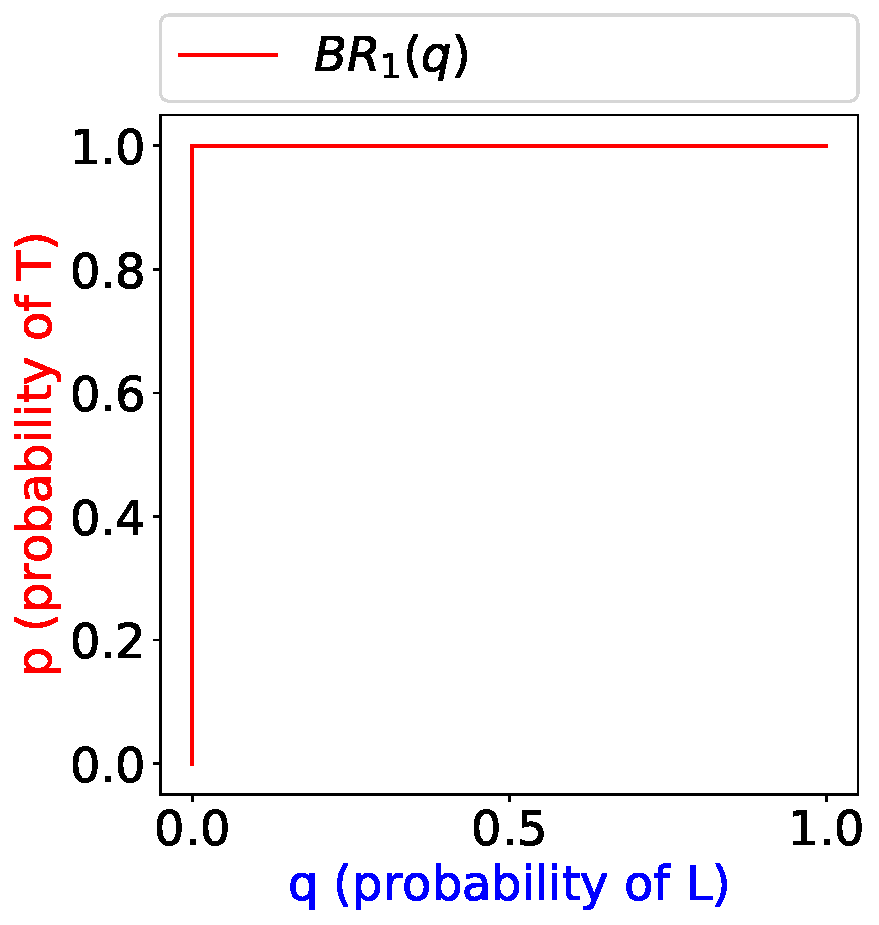
\includegraphics[width=\columnwidth]{figures/7c1}
    \textit{Write up Player 2's best-response (BR) function, $q^{*}(p)$}
  \vfill\null
  \end{multicols}
\end{frame}
\begin{frame}{PS3, Ex. 7.c: Mixed Strategy Nash Equilibria - (p,q)-diagrams}
  \begin{multicols}{2}
    \begin{itemize}
      \item[(c)] Plot the mixed best responses and find all NE (pure and mixed):
    \end{itemize}
    \vspace{-10pt}
    \begin{table}
      \begin{tabular}{cl|c|c|}
        & \multicolumn{1}{c}{} & \multicolumn{2}{c}{\color{blue}Player 2}\\
        \parbox[t]{1mm}{\multirow{3}{*}{\rotatebox[origin=r]{90}{\color{red}Player 1}}}
        & \multicolumn{1}{c}{} & \multicolumn{1}{c}{L ($q$)} & \multicolumn{1}{c}{R (1-$q$)} \\\cline{3-4}
        & T  ($p$)  & \textcolor{red}{3}, \textcolor{blue}{2} & \textcolor{red}{1}, \textcolor{blue}{2} \\\cline{3-4}
        & B  (1-$p$)& 0, 1 & \textcolor{red}{1}, \textcolor{blue}{2} \\\cline{3-4}
      \end{tabular}
    \end{table}
    Player 1 is indifferent if:
    \begin{align*}
      3q+(1-q) &= (1-q) \\
      q &= 0
    \end{align*}
    \vspace{-15pt}
    \begin{align*}
      BR_1(q)=\left\{ \begin{array}{lcl}
      p\in[0,1] & \text{if} & q=0 \\
      p=1       & \text{if} & q>0
      \end{array}\right.
    \end{align*}
    Player 2 is indifferent if:
    \begin{align*}
      2p + (1-p) &= 2 \\
      p + 1      &= 2 \Rightarrow p = 1
    \end{align*}
    \vspace{-15pt}
    \begin{align*}
      BR_2(p)=\left\{ \begin{array}{lcl}
      q=0       & \text{if} & p<1  \\
      q\in[0,1] & \text{if} & p=1
      \end{array}\right.
    \end{align*}
  \vfill\null \columnbreak
    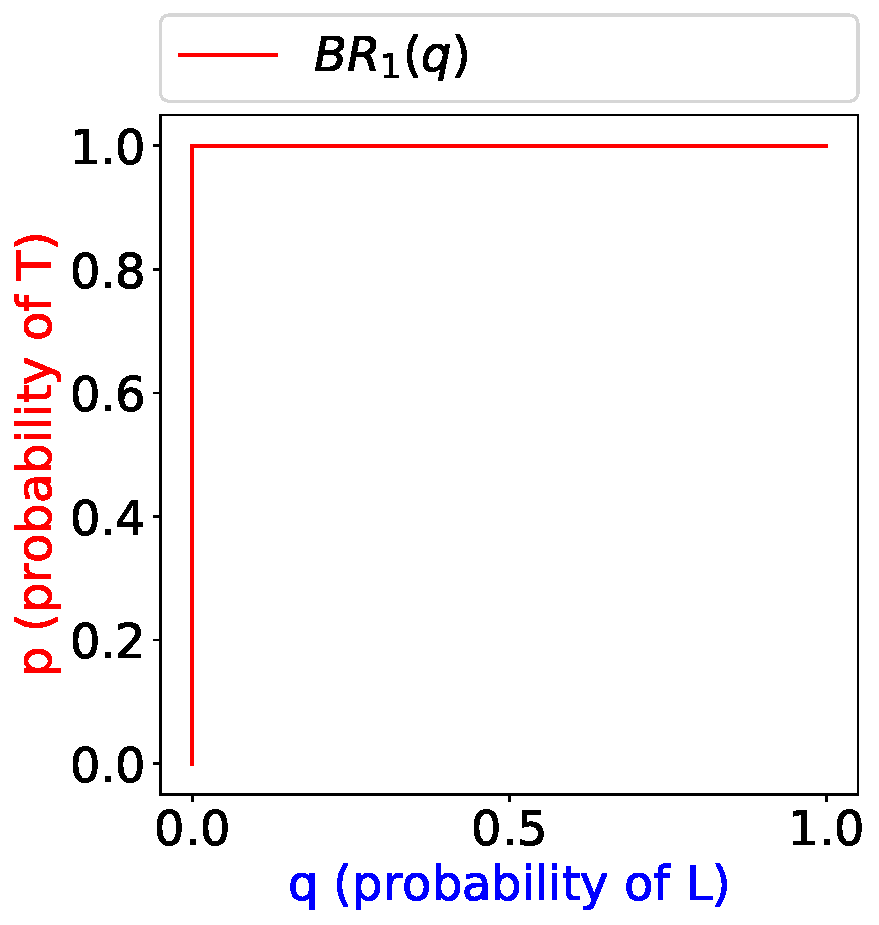
\includegraphics[width=\columnwidth]{figures/7c1}
    \textit{Plot Player 2's BR function, $q^{*}(p)$}
  \vfill\null
  \end{multicols}
\end{frame}
\begin{frame}{PS3, Ex. 7.c: Mixed Strategy Nash Equilibria - (p,q)-diagrams}
  \begin{multicols}{2}
    \begin{itemize}
      \item[(c)] Plot the mixed best responses and find all NE (pure and mixed):
    \end{itemize}
    \vspace{-10pt}
    \begin{table}
      \begin{tabular}{cl|c|c|}
        & \multicolumn{1}{c}{} & \multicolumn{2}{c}{\color{blue}Player 2}\\
        \parbox[t]{1mm}{\multirow{3}{*}{\rotatebox[origin=r]{90}{\color{red}Player 1}}}
        & \multicolumn{1}{c}{} & \multicolumn{1}{c}{L ($q$)} & \multicolumn{1}{c}{R (1-$q$)} \\\cline{3-4}
        & T  ($p$)  & \textcolor{red}{3}, \textcolor{blue}{2} & \textcolor{red}{1}, \textcolor{blue}{2} \\\cline{3-4}
        & B  (1-$p$)& 0, 1 & \textcolor{red}{1}, \textcolor{blue}{2} \\\cline{3-4}
      \end{tabular}
    \end{table}
    Player 1 is indifferent if:
    \begin{align*}
      3q+(1-q) &= (1-q) \\
      q &= 0
    \end{align*}
    \vspace{-15pt}
    \begin{align*}
      BR_1(q)=\left\{ \begin{array}{lcl}
      p\in[0,1] & \text{if} & q=0 \\
      p=1       & \text{if} & q>0
      \end{array}\right.
    \end{align*}
    Player 2 is indifferent if:
    \begin{align*}
      2p + (1-p) &= 2 \\
      p + 1      &= 2 \Rightarrow p = 1
    \end{align*}
    \vspace{-15pt}
    \begin{align*}
      BR_2(p)=\left\{ \begin{array}{lcl}
      q=0       & \text{if} & p<1  \\
      q\in[0,1] & \text{if} & p=1
      \end{array}\right.
    \end{align*}
  \vfill\null \columnbreak
    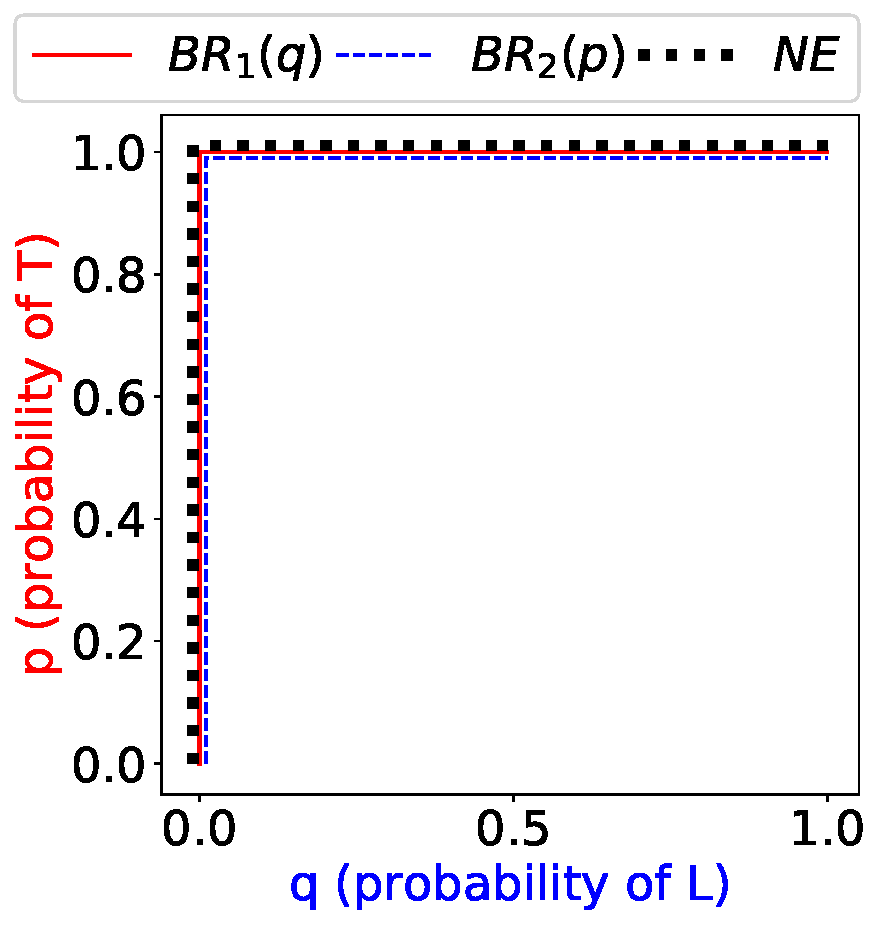
\includegraphics[width=\columnwidth]{figures/7c2}
    \textit{Write up all NE (pure and mixed).}
  \vfill\null
  \end{multicols}
\end{frame}
\begin{frame}{PS3, Ex. 7.c: Mixed Strategy Nash Equilibria - (p,q)-diagrams}
  \begin{multicols}{2}
    \begin{itemize}
      \item[(c)] Plot the mixed best responses and find all NE (pure and mixed):
    \end{itemize}
    \vspace{-10pt}
    \begin{table}
      \begin{tabular}{cl|c|c|}
        & \multicolumn{1}{c}{} & \multicolumn{2}{c}{\color{blue}Player 2}\\
        \parbox[t]{1mm}{\multirow{3}{*}{\rotatebox[origin=r]{90}{\color{red}Player 1}}}
        & \multicolumn{1}{c}{} & \multicolumn{1}{c}{L ($q$)} & \multicolumn{1}{c}{R (1-$q$)} \\\cline{3-4}
        & T  ($p$)  & \textcolor{red}{3}, \textcolor{blue}{2} & \textcolor{red}{1}, \textcolor{blue}{2} \\\cline{3-4}
        & B  (1-$p$)& 0, 1 & \textcolor{red}{1}, \textcolor{blue}{2} \\\cline{3-4}
      \end{tabular}
    \end{table}
    Player 1 is indifferent if:
    \begin{align*}
      3q+(1-q) &= (1-q) \\
      q &= 0
    \end{align*}
    \vspace{-15pt}
    \begin{align*}
      BR_1(q)=\left\{ \begin{array}{lcl}
      p\in[0,1] & \text{if} & q=0 \\
      p=1       & \text{if} & q>0
      \end{array}\right.
    \end{align*}
    Player 2 is indifferent if:
    \begin{align*}
      2p + (1-p) &= 2 \\
      p + 1      &= 2 \Rightarrow p = 1
    \end{align*}
    \vspace{-15pt}
    \begin{align*}
      BR_2(p)=\left\{ \begin{array}{lcl}
      q=0       & \text{if} & p<1  \\
      q\in[0,1] & \text{if} & p=1
      \end{array}\right.
    \end{align*}
  \vfill\null \columnbreak
    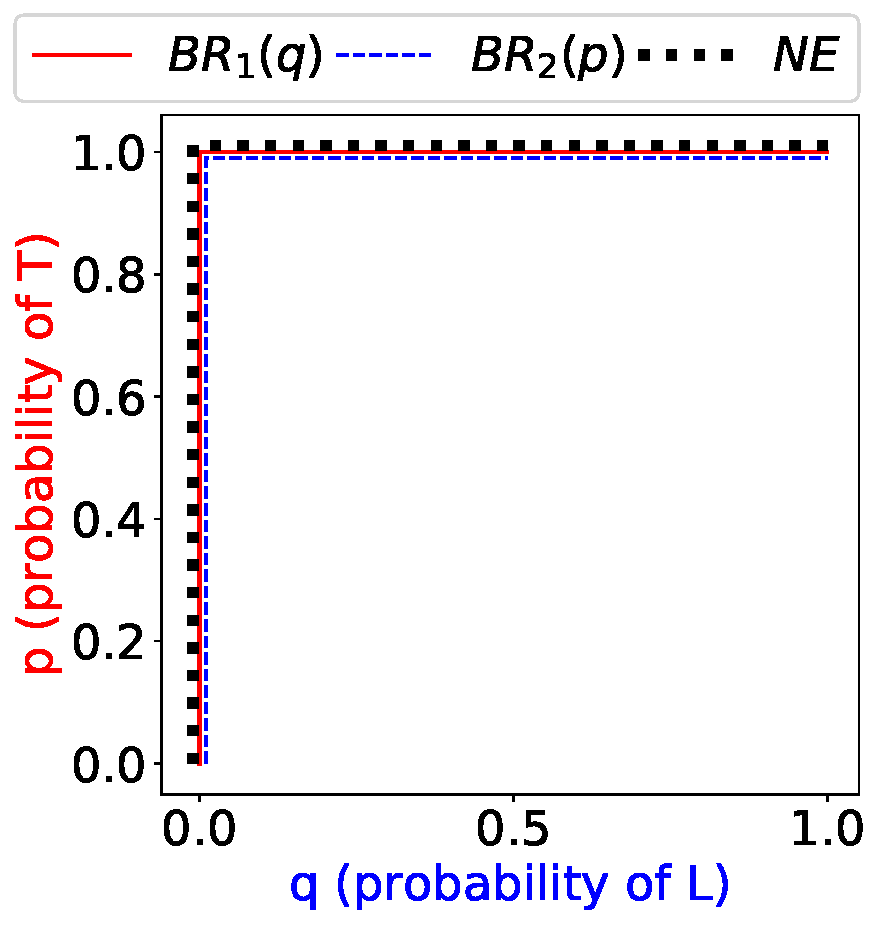
\includegraphics[width=\columnwidth]{figures/7c2}
    Three Pure Strategy NE (PSNE) exist:
    \begin{align*}
      PSNE=\{(T,L),(T,R),(B,R)\}
    \end{align*}
    \textit{What about Mixed Strategy NE (MSNE), $(p^{*},q^{*})$?}
  \vfill\null
  \end{multicols}
\end{frame}
\begin{frame}{PS3, Ex. 7.c: Mixed Strategy Nash Equilibria - (p,q)-diagrams}
  \begin{multicols}{2}
    \begin{itemize}
      \item[(c)] Plot the mixed best responses and find all NE (pure and mixed):
    \end{itemize}
    \vspace{-10pt}
    \begin{table}
      \begin{tabular}{cl|c|c|}
        & \multicolumn{1}{c}{} & \multicolumn{2}{c}{\color{blue}Player 2}\\
        \parbox[t]{1mm}{\multirow{3}{*}{\rotatebox[origin=r]{90}{\color{red}Player 1}}}
        & \multicolumn{1}{c}{} & \multicolumn{1}{c}{L ($q$)} & \multicolumn{1}{c}{R (1-$q$)} \\\cline{3-4}
        & T  ($p$)  & \textcolor{red}{3}, \textcolor{blue}{2} & \textcolor{red}{1}, \textcolor{blue}{2} \\\cline{3-4}
        & B  (1-$p$)& 0, 1 & \textcolor{red}{1}, \textcolor{blue}{2} \\\cline{3-4}
      \end{tabular}
    \end{table}
    Player 1 is indifferent if:
    \begin{align*}
      3q+(1-q) &= (1-q) \\
      q &= 0
    \end{align*}
    \vspace{-15pt}
    \begin{align*}
      BR_1(q)=\left\{ \begin{array}{lcl}
      p\in[0,1] & \text{if} & q=0 \\
      p=1       & \text{if} & q>0
      \end{array}\right.
    \end{align*}
    Player 2 is indifferent if:
    \begin{align*}
      2p + (1-p) &= 2 \\
      p + 1      &= 2 \Rightarrow p = 1
    \end{align*}
    \vspace{-15pt}
    \begin{align*}
      BR_2(p)=\left\{ \begin{array}{lcl}
      q=0       & \text{if} & p<1  \\
      q\in[0,1] & \text{if} & p=1
      \end{array}\right.
    \end{align*}
  \vfill\null \columnbreak
    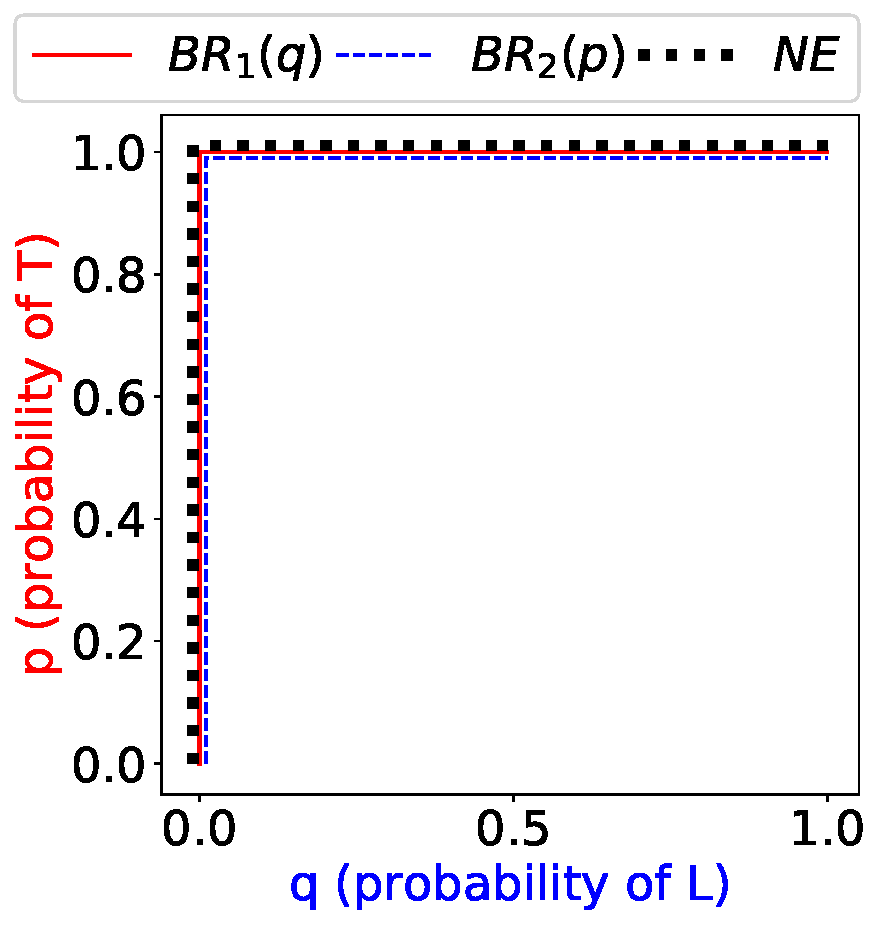
\includegraphics[width=\columnwidth]{figures/7c2}
    \begin{align*}
      PSNE=\{(T,L),(T,R),(B,R)\}
    \end{align*}
    The three PSNE are contained in the two mixed strategy NE (MSNE), $(p^{*},q^{*})$:
    \begin{align*}
      \left\{\left(p\in\left[0,1\right),q=0\right);\left(p=1,\in\left(0,1\right]\right)\right\}
    \end{align*}
  \vfill\null
  \end{multicols}
\end{frame}

\begin{frame}{PS3, Ex. 7.d: Mixed Strategy Nash Equilibria - (p,q)-diagrams}
  \begin{multicols}{2}
    \begin{itemize}
      \item[(d)] $PSNE=\{(s_1,t_1),(s_2,t_2)\}$
    \end{itemize}
    \vspace{-10pt}
    \begin{table}
      \begin{tabular}{l|c|c|}
          \multicolumn{1}{c}{}  & \multicolumn{1}{c}{$t_1$ ($q$)} & \multicolumn{1}{c}{$t_2$ (1-$q$)} \\\cline{2-3}
          $s_1$ ($p_1$)         & \textcolor{red}{2}, \textcolor{blue}{1} & 3, 0 \\\cline{2-3}
          $s_2$ ($p_2$)         & 1, 2 & \textcolor{red}{4}, \textcolor{blue}{3} \\\cline{2-3}
          $s_3$ (1-$p_1$-$p_2$) & 0, 1 & 0, \textcolor{blue}{3} \\\cline{2-3}
      \end{tabular}
    \end{table}
  \vfill\null \columnbreak
    \textit{Can we reduce the bi-matrix?}
  \vfill\null
  \end{multicols}
\end{frame}
\begin{frame}{PS3, Ex. 7.d: Mixed Strategy Nash Equilibria - (p,q)-diagrams}
  \begin{multicols}{2}
    \begin{itemize}
      \item[(d)] $PSNE=\{(s_1,t_1),(s_2,t_2)\}$
    \end{itemize}
    \begin{table}
      \begin{tabular}{l|c|c|}
          \multicolumn{1}{c}{}  & \multicolumn{1}{c}{$t_1$ ($q$)} & \multicolumn{1}{c}{$t_2$ (1-$q$)} \\\cline{2-3}
          $s_1$ ($p_1$)         & \textcolor{red}{2}, \textcolor{blue}{1} & 3, 0 \\\cline{2-3}
          $s_2$ ($p_2$)         & 1, 2 & \textcolor{red}{4}, \textcolor{blue}{3} \\\cline{2-3}
          $s_3$ (1-$p_1$-$p_2$) & 0, 1 & 0, \textcolor{blue}{3} \\\cline{2-3}
      \end{tabular}
    \end{table}
    \textbf{IESDS}: $s_2>s_3$, thus $s_3$ can be eliminated and 1-$p_1$-$p_2=0\Rightarrow p_2=1-p_1$
    \begin{table}
      \begin{tabular}{cl|c|c|}
        & \multicolumn{1}{c}{} & \multicolumn{2}{c}{\color{blue}Player 2}\\
        \parbox[t]{1mm}{\multirow{3}{*}{\rotatebox[origin=r]{90}{\color{red}Player 1}}}
        & \multicolumn{1}{c}{}  & \multicolumn{1}{c}{$t_1$ ($q$)} & \multicolumn{1}{c}{$t_2$ (1-$q$)} \\\cline{3-4}
        & $s_1$ ($p_1$)  & \textcolor{red}{2}, \textcolor{blue}{1} & 3, 0 \\\cline{3-4}
        & $s_2$ (1-$p_1$)& 1, 2 & \textcolor{red}{4}, \textcolor{blue}{3} \\\cline{3-4}
      \end{tabular}
    \end{table}
  \vfill\null \columnbreak
    \textit{For which values of $q$ is Player 1 indifferent?}
  \vfill\null
  \end{multicols}
\end{frame}
\begin{frame}{PS3, Ex. 7.d: Mixed Strategy Nash Equilibria - (p,q)-diagrams}
  \begin{multicols}{2}
    \begin{itemize}
      \item[(d)] $PSNE=\{(s_1,t_1),(s_2,t_2)\}$
    \end{itemize}
    \vspace{-8pt}
    \begin{table}
      \begin{tabular}{l|c|c|}
          \multicolumn{1}{c}{}  & \multicolumn{1}{c}{$t_1$ ($q$)} & \multicolumn{1}{c}{$t_2$ (1-$q$)} \\\cline{2-3}
          $s_1$ ($p_1$)         & \textcolor{red}{2}, \textcolor{blue}{1} & 3, 0 \\\cline{2-3}
          $s_2$ ($p_2$)         & 1, 2 & \textcolor{red}{4}, \textcolor{blue}{3} \\\cline{2-3}
          $s_3$ (1-$p_1$-$p_2$) & 0, 1 & 0, \textcolor{blue}{3} \\\cline{2-3}
      \end{tabular}
    \end{table}
    \vspace{-2pt}
    \textbf{IESDS}: $s_2>s_3$, thus $s_3$ can be eliminated and 1-$p_1$-$p_2=0\Rightarrow p_2=1-p_1$
    \vspace{-6pt}
    \begin{table}
      \begin{tabular}{cl|c|c|}
        & \multicolumn{1}{c}{} & \multicolumn{2}{c}{\color{blue}Player 2}\\
        \parbox[t]{1mm}{\multirow{3}{*}{\rotatebox[origin=r]{90}{\color{red}Player 1}}}
        & \multicolumn{1}{c}{}  & \multicolumn{1}{c}{$t_1$ ($q$)} & \multicolumn{1}{c}{$t_2$ (1-$q$)} \\\cline{3-4}
        & $s_1$ ($p_1$)  & \textcolor{red}{2}, \textcolor{blue}{1} & 3, 0 \\\cline{3-4}
        & $s_2$ (1-$p_1$)& 1, 2 & \textcolor{red}{4}, \textcolor{blue}{3} \\\cline{3-4}
      \end{tabular}
    \end{table}
    Player 1 is indifferent if:
    \begin{align*}
      2q+3(1-q) &= q+4(1-q) \\
      q &= 1-q \Rightarrow q = \frac{1}{2}
    \end{align*}
  \vfill\null \columnbreak
    \textit{For which values of $p$ is Player 2 indifferent?}
  \vfill\null
  \end{multicols}
\end{frame}
\begin{frame}{PS3, Ex. 7.d: Mixed Strategy Nash Equilibria - (p,q)-diagrams}
  \begin{multicols}{2}
    \begin{itemize}
      \item[(d)] $PSNE=\{(s_1,t_1),(s_2,t_2)\}$
    \end{itemize}
    \vspace{-8pt}
    \begin{table}
      \begin{tabular}{l|c|c|}
          \multicolumn{1}{c}{}  & \multicolumn{1}{c}{$t_1$ ($q$)} & \multicolumn{1}{c}{$t_2$ (1-$q$)} \\\cline{2-3}
          $s_1$ ($p_1$)         & \textcolor{red}{2}, \textcolor{blue}{1} & 3, 0 \\\cline{2-3}
          $s_2$ ($p_2$)         & 1, 2 & \textcolor{red}{4}, \textcolor{blue}{3} \\\cline{2-3}
          $s_3$ (1-$p_1$-$p_2$) & 0, 1 & 0, \textcolor{blue}{3} \\\cline{2-3}
      \end{tabular}
    \end{table}
    \vspace{-2pt}
    \textbf{IESDS}: $s_2>s_3$, thus $s_3$ can be eliminated and 1-$p_1$-$p_2=0\Rightarrow p_2=1-p_1$
    \vspace{-6pt}
    \begin{table}
      \begin{tabular}{cl|c|c|}
        & \multicolumn{1}{c}{} & \multicolumn{2}{c}{\color{blue}Player 2}\\
        \parbox[t]{1mm}{\multirow{3}{*}{\rotatebox[origin=r]{90}{\color{red}Player 1}}}
        & \multicolumn{1}{c}{}  & \multicolumn{1}{c}{$t_1$ ($q$)} & \multicolumn{1}{c}{$t_2$ (1-$q$)} \\\cline{3-4}
        & $s_1$ ($p_1$)  & \textcolor{red}{2}, \textcolor{blue}{1} & 3, 0 \\\cline{3-4}
        & $s_2$ (1-$p_1$)& 1, 2 & \textcolor{red}{4}, \textcolor{blue}{3} \\\cline{3-4}
      \end{tabular}
    \end{table}
    Player 1 is indifferent if:
    \begin{align*}
      2q+3(1-q) &= q+4(1-q) \\
      q &= 1-q \Rightarrow q = \frac{1}{2}
    \end{align*}
    Player 2 is indifferent if:
    \begin{align*}
      p_1 + 2(1-p_1)  &= 3(1-p_1) \\
      p_1             &= 1-p_1 \Rightarrow p_1 = \frac{1}{2}
    \end{align*}
  \vfill\null \columnbreak
    \textit{Plot Player 1's BR function, $p^{*}(q)$, in a (p,q)-diagram.}
  \vfill\null
  \end{multicols}
\end{frame}
\begin{frame}{PS3, Ex. 7.d: Mixed Strategy Nash Equilibria - (p,q)-diagrams}
  \begin{multicols}{2}
    \begin{itemize}
      \item[(d)] $PSNE=\{(s_1,t_1),(s_2,t_2)\}$
    \end{itemize}
    \vspace{-8pt}
    \begin{table}
      \begin{tabular}{l|c|c|}
          \multicolumn{1}{c}{}  & \multicolumn{1}{c}{$t_1$ ($q$)} & \multicolumn{1}{c}{$t_2$ (1-$q$)} \\\cline{2-3}
          $s_1$ ($p_1$)         & \textcolor{red}{2}, \textcolor{blue}{1} & 3, 0 \\\cline{2-3}
          $s_2$ ($p_2$)         & 1, 2 & \textcolor{red}{4}, \textcolor{blue}{3} \\\cline{2-3}
          $s_3$ (1-$p_1$-$p_2$) & 0, 1 & 0, \textcolor{blue}{3} \\\cline{2-3}
      \end{tabular}
    \end{table}
    \vspace{-2pt}
    \textbf{IESDS}: $s_2>s_3$, thus $s_3$ can be eliminated and 1-$p_1$-$p_2=0\Rightarrow p_2=1-p_1$
    \vspace{-6pt}
    \begin{table}
      \begin{tabular}{cl|c|c|}
        & \multicolumn{1}{c}{} & \multicolumn{2}{c}{\color{blue}Player 2}\\
        \parbox[t]{1mm}{\multirow{3}{*}{\rotatebox[origin=r]{90}{\color{red}Player 1}}}
        & \multicolumn{1}{c}{}  & \multicolumn{1}{c}{$t_1$ ($q$)} & \multicolumn{1}{c}{$t_2$ (1-$q$)} \\\cline{3-4}
        & $s_1$ ($p_1$)  & \textcolor{red}{2}, \textcolor{blue}{1} & 3, 0 \\\cline{3-4}
        & $s_2$ (1-$p_1$)& 1, 2 & \textcolor{red}{4}, \textcolor{blue}{3} \\\cline{3-4}
      \end{tabular}
    \end{table}
    Player 1 is indifferent if:
    \begin{align*}
      2q+3(1-q) &= q+4(1-q) \\
      q &= 1-q \Rightarrow q = \frac{1}{2}
    \end{align*}
    Player 2 is indifferent if:
    \begin{align*}
      p_1 + 2(1-p_1)  &= 3(1-p_1) \\
      p_1             &= 1-p_1 \Rightarrow p_1 = \frac{1}{2}
    \end{align*}
  \vfill\null \columnbreak
    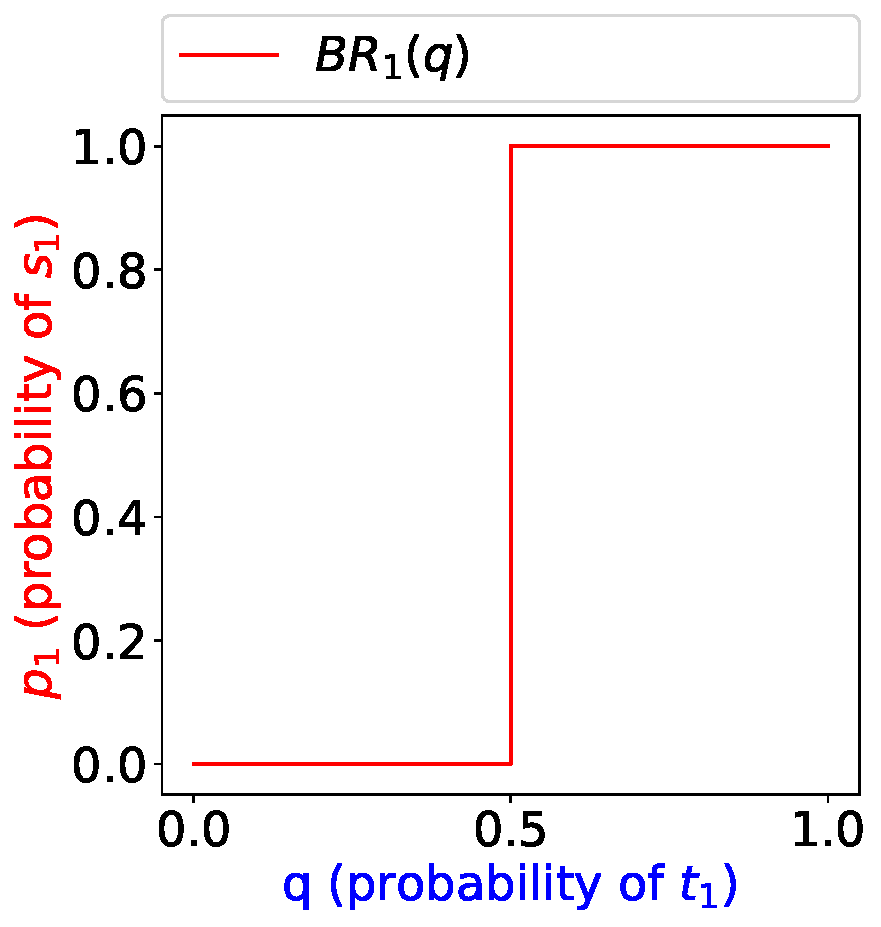
\includegraphics[width=\columnwidth]{figures/7d1}
    \textit{Plot Player 2's BR function, $q^{*}(p)$}
  \vfill\null
  \end{multicols}
\end{frame}
\begin{frame}{PS3, Ex. 7.d: Mixed Strategy Nash Equilibria - (p,q)-diagrams}
  \begin{multicols}{2}
    \begin{itemize}
      \item[(d)] $PSNE=\{(s_1,t_1),(s_2,t_2)\}$
    \end{itemize}
    \vspace{-8pt}
    \begin{table}
      \begin{tabular}{l|c|c|}
          \multicolumn{1}{c}{}  & \multicolumn{1}{c}{$t_1$ ($q$)} & \multicolumn{1}{c}{$t_2$ (1-$q$)} \\\cline{2-3}
          $s_1$ ($p_1$)         & \textcolor{red}{2}, \textcolor{blue}{1} & 3, 0 \\\cline{2-3}
          $s_2$ ($p_2$)         & 1, 2 & \textcolor{red}{4}, \textcolor{blue}{3} \\\cline{2-3}
          $s_3$ (1-$p_1$-$p_2$) & 0, 1 & 0, \textcolor{blue}{3} \\\cline{2-3}
      \end{tabular}
    \end{table}
    \vspace{-2pt}
    \textbf{IESDS}: $s_2>s_3$, thus $s_3$ can be eliminated and 1-$p_1$-$p_2=0\Rightarrow p_2=1-p_1$
    \vspace{-6pt}
    \begin{table}
      \begin{tabular}{cl|c|c|}
        & \multicolumn{1}{c}{} & \multicolumn{2}{c}{\color{blue}Player 2}\\
        \parbox[t]{1mm}{\multirow{3}{*}{\rotatebox[origin=r]{90}{\color{red}Player 1}}}
        & \multicolumn{1}{c}{}  & \multicolumn{1}{c}{$t_1$ ($q$)} & \multicolumn{1}{c}{$t_2$ (1-$q$)} \\\cline{3-4}
        & $s_1$ ($p_1$)  & \textcolor{red}{2}, \textcolor{blue}{1} & 3, 0 \\\cline{3-4}
        & $s_2$ (1-$p_1$)& 1, 2 & \textcolor{red}{4}, \textcolor{blue}{3} \\\cline{3-4}
      \end{tabular}
    \end{table}
    Player 1 is indifferent if:
    \begin{align*}
      2q+3(1-q) &= q+4(1-q) \\
      q &= 1-q \Rightarrow q = \frac{1}{2}
    \end{align*}
    Player 2 is indifferent if:
    \begin{align*}
      p_1 + 2(1-p_1)  &= 3(1-p_1) \\
      p_1             &= 1-p_1 \Rightarrow p_1 = \frac{1}{2}
    \end{align*}
  \vfill\null \columnbreak
    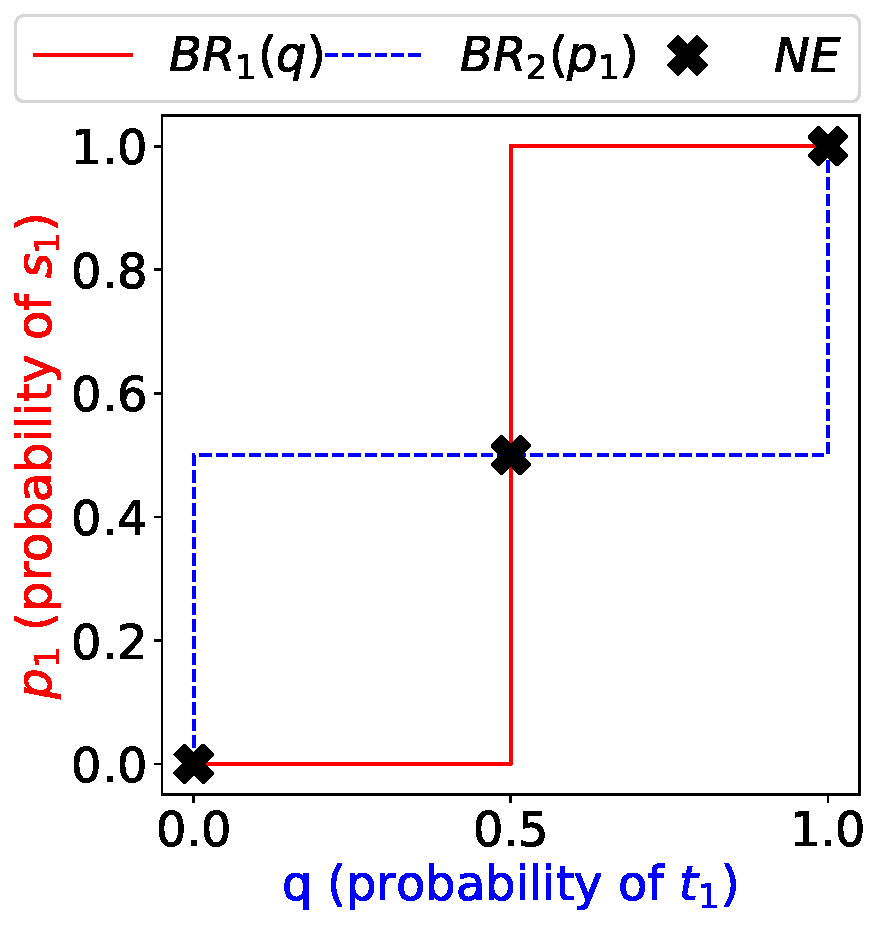
\includegraphics[width=\columnwidth]{figures/7d2}
    \textit{Write up all NE (pure and mixed), both in the reduced game and in the full game.}
  \vfill\null
  \end{multicols}
\end{frame}
\begin{frame}{PS3, Ex. 7.d: Mixed Strategy Nash Equilibria - (p,q)-diagrams}
  \begin{multicols}{2}
    \begin{itemize}
      \item[(d)] $PSNE=\{(s_1,t_1),(s_2,t_2)\}$
    \end{itemize}
    \vspace{-10pt}
    \begin{table}
      \begin{tabular}{l|c|c|}
          \multicolumn{1}{c}{}  & \multicolumn{1}{c}{$t_1$ ($q$)} & \multicolumn{1}{c}{$t_2$ (1-$q$)} \\\cline{2-3}
          $s_1$ ($p_1$)         & \textcolor{red}{2}, \textcolor{blue}{1} & 3, 0 \\\cline{2-3}
          $s_2$ ($p_2$)         & 1, 2 & \textcolor{red}{4}, \textcolor{blue}{3} \\\cline{2-3}
          $s_3$ (1-$p_1$-$p_2$) & 0, 1 & 0, \textcolor{blue}{3} \\\cline{2-3}
      \end{tabular}
    \end{table}
    \vspace{-4pt}
    \textbf{IESDS}: $s_2>s_3$, thus $s_3$ can be eliminated and 1-$p_1$-$p_2=0\Rightarrow p_2=1-p_1$
    \vspace{-6pt}
    \begin{table}
      \begin{tabular}{cl|c|c|}
        & \multicolumn{1}{c}{} & \multicolumn{2}{c}{\color{blue}Player 2}\\
        \parbox[t]{1mm}{\multirow{3}{*}{\rotatebox[origin=r]{90}{\color{red}Player 1}}}
        & \multicolumn{1}{c}{}  & \multicolumn{1}{c}{$t_1$ ($q$)} & \multicolumn{1}{c}{$t_2$ (1-$q$)} \\\cline{3-4}
        & $s_1$ ($p_1$)  & \textcolor{red}{2}, \textcolor{blue}{1} & 3, 0 \\\cline{3-4}
        & $s_2$ (1-$p_1$)& 1, 2 & \textcolor{red}{4}, \textcolor{blue}{3} \\\cline{3-4}
      \end{tabular}
    \end{table}
    \vspace{-2pt}
    Player 1 is indifferent if:
    \vspace{-4pt}
    \begin{align*}
      2q+3(1-q) &= q+4(1-q) \\
      q &= 1-q \Rightarrow q = \frac{1}{2}
    \end{align*}
    Player 2 is indifferent if:
    \vspace{-4pt}
    \begin{align*}
      p_1 + 2(1-p_1)  &= 3(1-p_1) \\
      p_1             &= 1-p_1 \Rightarrow p_1 = \frac{1}{2}
    \end{align*}
  \vfill\null \columnbreak
    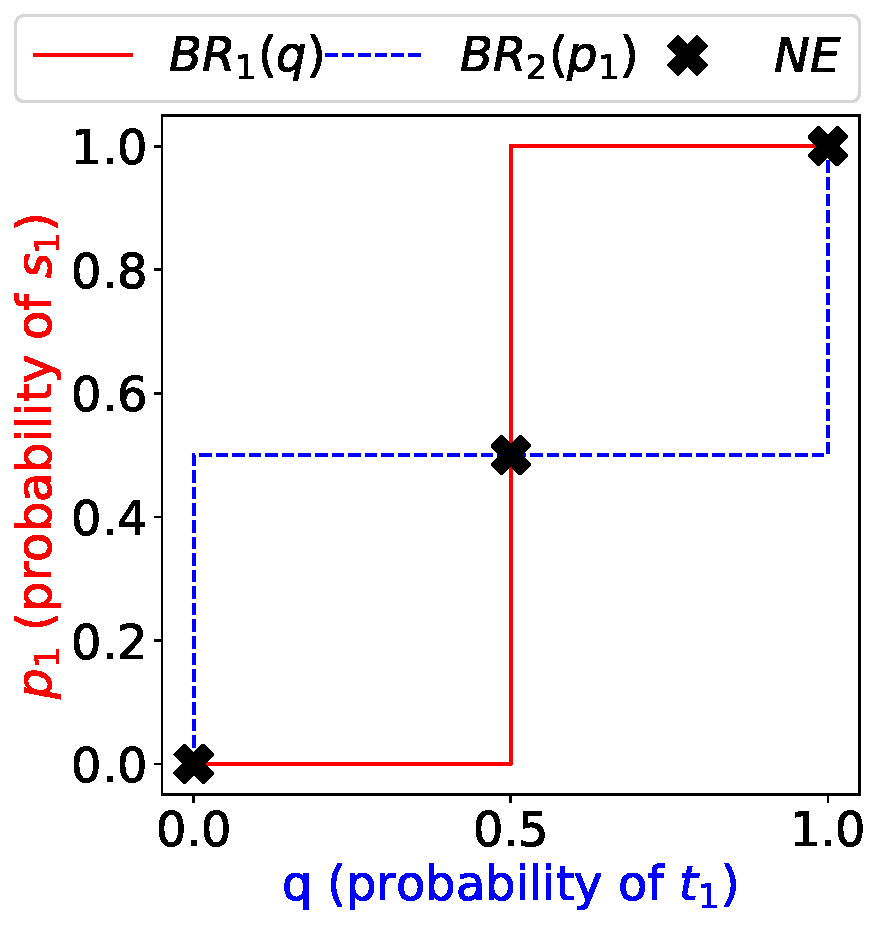
\includegraphics[width=\columnwidth]{figures/7d2}
    In the reduced game, three NE exist:
    \begin{align*}
      (p_1^{*},q^{*})=\left\{(0,0),(1/2,1/2),(1,1)\right\}
    \end{align*}
    And in the full game: $\left[(p_1^{*},p_2^{*}),(q^{*})\right]=$
    \begin{align*}
      \left\{\left[(0,1),(0)\right];\left[\left(\frac{1}{2},\frac{1}{2}\right),\left(\frac{1}{2}\right)\right];\left[(1,0),(1)\right]\right\}
    \end{align*}
  \vfill\null
  \end{multicols}
\end{frame}


\section{PS3, Ex. 8: Mixed Strategy Nash Equilibria - analytical solution}

\begin{frame}{PS3, Ex. 8: Mixed Strategy Nash Equilibria - analytical solution}
  Find all (pure and mixed) Nash equilibria in the following game:
    \begin{table}
      \begin{tabular}{l|c|c|c|}
          \multicolumn{1}{c}{}  & \multicolumn{1}{c}{L ($q_1$)} & \multicolumn{1}{c}{C ($q_2$)} & \multicolumn{1}{c}{R (1-$q_1$-$q_2$)} \\\cline{2-4}
          T ($p$)   & 4, 1 & 2, 3 & 0, 4 \\\cline{2-4}
          B (1-$p$) & 2, 3 & 1, 2 & 5, 0 \\\cline{2-4}
      \end{tabular}
    \end{table}
  \vfill\null
\end{frame}
\begin{frame}{PS3, Ex. 8: Mixed Strategy Nash Equilibria - analytical solution}
  Find all (pure and mixed) Nash equilibria in the following game:
    \begin{table}
      \begin{tabular}{l|c|c|c|}
          \multicolumn{1}{c}{}  & \multicolumn{1}{c}{L ($q_1$)} & \multicolumn{1}{c}{C ($q_2$)} & \multicolumn{1}{c}{R (1-$q_1$-$q_2$)} \\\cline{2-4}
          T ($p$)   & 4, 1 & 2, 3 & 0, 4 \\\cline{2-4}
          B (1-$p$) & 2, 3 & 1, 2 & 5, 0 \\\cline{2-4}
      \end{tabular}
    \end{table}
    \textbf{Hints:}
    \begin{enumerate}
      \item Highlight the best responses in the matrix.
      \item Find the relationship between $q_1$ and $q_2$ for which \textbf{Player 1 is indifferent}.
      \item Write up the \textbf{best responses for Player 1}: $p^{*}(q_1,q_2)$, i.e. $BR_1(q_1,q_2)$.
      \item Pairwise find the probabilities $p$ for which \textbf{Player 2 is indifferent}, e.g. between $L$ and $C$, then $L$ and $R$, and finally between $C$ and $R$.
      \item Write up the \textbf{best responses for Player 2}:
      \begin{align*}
        BR_2(p)=\left(q_1^{*}(p),q_2^{*}(p)\right)=\left\{ \begin{array}{ll}
            \vdots              & \vdots  \\
            \{(0,x):x\in[0,1]\} & p = 2/3 \\
            (0,0)               & p > 2/3 \\
        \end{array}\right.
      \end{align*}
      \item \textbf{Find the NE} (pure and mixed). In a Mixed Strategy Nash Equilibriumm (MSNE) both players must be indifferent between their respective pure strategies.
    \end{enumerate}
  \vfill\null
\end{frame}
\begin{frame}{PS3, Ex. 8: Mixed Strategy Nash Equilibria - analytical solution}
  \begin{multicols}{2}
    \begin{itemize}
      \item[1.] Highlight the best responses in the matrix:
    \end{itemize}
    \vspace{-15pt}
    \begin{table}
      \begin{tabular}{l|c|c|c|}
          \multicolumn{1}{c}{}  & \multicolumn{1}{c}{L ($q_1$)} & \multicolumn{1}{c}{C ($q_2$)} & \multicolumn{1}{c}{R (1-$q_1$-$q_2$)} \\\cline{2-4}
          T ($p$)   & 4, 1 & 2, 3 & 0, 4 \\\cline{2-4}
          B (1-$p$) & 2, 3 & 1, 2 & 5, 0 \\\cline{2-4}
      \end{tabular}
    \end{table}
    \textit{Which Pure Strategy Nash Equilibria (PSNE) exist?}
  \vfill\null \columnbreak
  \vfill\null
  \end{multicols}
\end{frame}
\begin{frame}{PS3, Ex. 8: Mixed Strategy Nash Equilibria - analytical solution}
  \begin{multicols}{2}
    \begin{itemize}
      \item[1.] Highlight the best responses in the matrix:
    \end{itemize}
    \vspace{-15pt}
    \begin{table}
      \begin{tabular}{l|c|c|c|}
          \multicolumn{1}{c}{}  & \multicolumn{1}{c}{L ($q_1$)} & \multicolumn{1}{c}{C ($q_2$)} & \multicolumn{1}{c}{R (1-$q_1$-$q_2$)} \\\cline{2-4}
          T ($p$)   & \textcolor{red}{4}, 1 & \textcolor{red}{2}, 3 & 0, \textcolor{blue}{4} \\\cline{2-4}
          B (1-$p$) & 2, \textcolor{blue}{3} & 1, 2 & \textcolor{red}{5}, 0 \\\cline{2-4}
      \end{tabular}
    \end{table}
    No Pure Strategy Nash Equilibrium (PSNE) exist.
  \vfill\null \columnbreak
  \vfill\null
  \end{multicols}
\end{frame}
\begin{frame}{PS3, Ex. 8: Mixed Strategy Nash Equilibria - analytical solution}
  \begin{multicols}{2}
    \begin{table}
      \begin{tabular}{l|c|c|c|}
          \multicolumn{1}{c}{}  & \multicolumn{1}{c}{L ($q_1$)} & \multicolumn{1}{c}{C ($q_2$)} & \multicolumn{1}{c}{R (1-$q_1$-$q_2$)} \\\cline{2-4}
          T ($p$)   & \textcolor{red}{4}, 1 & \textcolor{red}{2}, 3 & 0, \textcolor{blue}{4} \\\cline{2-4}
          B (1-$p$) & 2, \textcolor{blue}{3} & 1, 2 & \textcolor{red}{5}, 0 \\\cline{2-4}
      \end{tabular}
    \end{table}
    No Pure Strategy Nash Equilibrium (PSNE) exist.
    \begin{itemize}
      \item[2.] Find the relationship between $q_1$ and $q_2$ for which \textbf{Player 1 is indifferent}.
    \end{itemize}
  \vfill\null \columnbreak
  \vfill\null
  \end{multicols}
\end{frame}
\begin{frame}{PS3, Ex. 8: Mixed Strategy Nash Equilibria - analytical solution}
  \begin{multicols}{2}
    \begin{table}
      \begin{tabular}{l|c|c|c|}
          \multicolumn{1}{c}{}  & \multicolumn{1}{c}{L ($q_1$)} & \multicolumn{1}{c}{C ($q_2$)} & \multicolumn{1}{c}{R (1-$q_1$-$q_2$)} \\\cline{2-4}
          T ($p$)   & \textcolor{red}{4}, 1 & \textcolor{red}{2}, 3 & 0, \textcolor{blue}{4} \\\cline{2-4}
          B (1-$p$) & 2, \textcolor{blue}{3} & 1, 2 & \textcolor{red}{5}, 0 \\\cline{2-4}
      \end{tabular}
    \end{table}
    \begin{itemize}
      \item[2.] Find the relationship between $q_1$ and $q_2$ for which \textbf{Player 1 is indifferent}:
    \end{itemize}
    Player 1 is indifferent if:
    \begin{align*}
      4q_1 + 2q_2 &= 2q_1 + q_2 + 5(1-q_1-q_2)\\
      7q_1 + 6q_2 &= 5 \\
      q_1 + \frac{6}{7}q_2 &= \frac{5}{7}
    \end{align*}
  \vfill\null \columnbreak
  \vfill\null
  \end{multicols}
\end{frame}
\begin{frame}{PS3, Ex. 8: Mixed Strategy Nash Equilibria - analytical solution}
  \begin{multicols}{2}
    \begin{table}
      \begin{tabular}{l|c|c|c|}
          \multicolumn{1}{c}{}  & \multicolumn{1}{c}{L ($q_1$)} & \multicolumn{1}{c}{C ($q_2$)} & \multicolumn{1}{c}{R (1-$q_1$-$q_2$)} \\\cline{2-4}
          T ($p$)   & \textcolor{red}{4}, 1 & \textcolor{red}{2}, 3 & 0, \textcolor{blue}{4} \\\cline{2-4}
          B (1-$p$) & 2, \textcolor{blue}{3} & 1, 2 & \textcolor{red}{5}, 0 \\\cline{2-4}
      \end{tabular}
    \end{table}
    Player 1 is indifferent if:
    \begin{align*}
      4q_1 + 2q_2 &= 2q_1 + q_2 + 5(1-q_1-q_2)\\
      7q_1 + 6q_2 &= 5 \\
      q_1 + \frac{6}{7}q_2 &= \frac{5}{7}
    \end{align*}
    \begin{itemize}
      \item[3.] Write up the \textbf{best responses for Player 1}: $p^{*}(q_1,q_2)=$
    \end{itemize}
  \vfill\null \columnbreak
  \vfill\null
  \end{multicols}
\end{frame}
\begin{frame}{PS3, Ex. 8: Mixed Strategy Nash Equilibria - analytical solution}
  \begin{multicols}{2}
    \begin{table}
      \begin{tabular}{l|c|c|c|}
          \multicolumn{1}{c}{}  & \multicolumn{1}{c}{L ($q_1$)} & \multicolumn{1}{c}{C ($q_2$)} & \multicolumn{1}{c}{R (1-$q_1$-$q_2$)} \\\cline{2-4}
          T ($p$)   & \textcolor{red}{4}, 1 & \textcolor{red}{2}, 3 & 0, \textcolor{blue}{4} \\\cline{2-4}
          B (1-$p$) & 2, \textcolor{blue}{3} & 1, 2 & \textcolor{red}{5}, 0 \\\cline{2-4}
      \end{tabular}
    \end{table}
    Player 1 is indifferent if:
    \begin{align*}
      4q_1 + 2q_2 &= 2q_1 + q_2 + 5(1-q_1-q_2)\\
      7q_1 + 6q_2 &= 5 \\
      q_1 + \frac{6}{7}q_2 &= \frac{5}{7}
    \end{align*}
    \begin{itemize}
      \item[3.] Write up the \textbf{best responses for Player 1}: $p^{*}(q_1,q_2)=$, i.e.
    \end{itemize}
    \begin{align*}
      BR_1(q_1,q_2)=\left\{ \begin{array}{ll}
          1                 & q_1 + \frac{6}{7}q_2 > \frac{5}{7} \\
          \left[0,1\right]  & q_1 + \frac{6}{7}q_2 = \frac{5}{7} \\
          0                 & q_1 + \frac{6}{7}q_2 < \frac{5}{7}
      \end{array}\right.
    \end{align*}
  \vfill\null \columnbreak
  \vfill\null
  \end{multicols}
\end{frame}
\begin{frame}{PS3, Ex. 8: Mixed Strategy Nash Equilibria - analytical solution}
  \begin{multicols}{2}
    \begin{table}
      \begin{tabular}{l|c|c|c|}
          \multicolumn{1}{c}{}  & \multicolumn{1}{c}{L ($q_1$)} & \multicolumn{1}{c}{C ($q_2$)} & \multicolumn{1}{c}{R (1-$q_1$-$q_2$)} \\\cline{2-4}
          T ($p$)   & \textcolor{red}{4}, 1 & \textcolor{red}{2}, 3 & 0, \textcolor{blue}{4} \\\cline{2-4}
          B (1-$p$) & 2, \textcolor{blue}{3} & 1, 2 & \textcolor{red}{5}, 0 \\\cline{2-4}
      \end{tabular}
    \end{table}
    Player 1's best responses: $p^{*}(q_1,q_2)$, i.e.
    \begin{align*}
      BR_1(q_1,q_2)=\left\{ \begin{array}{ll}
          1                 & q_1 + \frac{6}{7}q_2 > \frac{5}{7}\\
          \left[0,1\right]  & q_1 + \frac{6}{7}q_2 = \frac{5}{7}\\
          0                 & q_1 + \frac{6}{7}q_2 < \frac{5}{7}
      \end{array}\right.
    \end{align*}
    \begin{itemize}
      \item[4.] Pairwise find the probabilities $p$ for which \textbf{Player 2 is indifferent}, e.g. between $L$ and $C$, then $L$ and $R$, and finally between $C$ and $R$.
    \end{itemize}
  \vfill\null \columnbreak
  \vfill\null
  \end{multicols}
\end{frame}
\begin{frame}{PS3, Ex. 8: Mixed Strategy Nash Equilibria - analytical solution}
  \begin{multicols}{2}
    \begin{table}
      \begin{tabular}{l|c|c|c|}
          \multicolumn{1}{c}{}  & \multicolumn{1}{c}{L ($q_1$)} & \multicolumn{1}{c}{C ($q_2$)} & \multicolumn{1}{c}{R (1-$q_1$-$q_2$)} \\\cline{2-4}
          T ($p$)   & \textcolor{red}{4}, 1 & \textcolor{red}{2}, 3 & 0, \textcolor{blue}{4} \\\cline{2-4}
          B (1-$p$) & 2, \textcolor{blue}{3} & 1, 2 & \textcolor{red}{5}, 0 \\\cline{2-4}
      \end{tabular}
    \end{table}
    Player 1's best responses: $p^{*}(q_1,q_2)$, i.e.
    \begin{align*}
      BR_1(q_1,q_2)=\left\{ \begin{array}{ll}
          1                 & q_1 + \frac{6}{7}q_2 > \frac{5}{7}\\
          \left[0,1\right]  & q_1 + \frac{6}{7}q_2 = \frac{5}{7}\\
          0                 & q_1 + \frac{6}{7}q_2 < \frac{5}{7}
      \end{array}\right.
    \end{align*}
    \begin{itemize}
      \item[4.] Pairwise find the probabilities $p$ for which \textbf{Player 2 is indifferent}, e.g. between $L$ and $C$, then $L$ and $R$, and finally between $C$ and $R$.
    \end{itemize}
  \vfill\null \columnbreak
    Player 2 is indifferent between $L$ and $C$ if:
    \begin{align*}
      p+3(1-p)&= 3p + 2(1-p) \\
      1-p     &= 2p \\
      p       &= \frac{1}{3}
    \end{align*}
    If $p<1/3$ prefer $L$; if $p>1/3$ prefer $C$.\\\medskip
  \vfill\null
  \end{multicols}
\end{frame}
\begin{frame}{PS3, Ex. 8: Mixed Strategy Nash Equilibria - analytical solution}
  \begin{multicols}{2}
    \begin{table}
      \begin{tabular}{l|c|c|c|}
          \multicolumn{1}{c}{}  & \multicolumn{1}{c}{L ($q_1$)} & \multicolumn{1}{c}{C ($q_2$)} & \multicolumn{1}{c}{R (1-$q_1$-$q_2$)} \\\cline{2-4}
          T ($p$)   & \textcolor{red}{4}, 1 & \textcolor{red}{2}, 3 & 0, \textcolor{blue}{4} \\\cline{2-4}
          B (1-$p$) & 2, \textcolor{blue}{3} & 1, 2 & \textcolor{red}{5}, 0 \\\cline{2-4}
      \end{tabular}
    \end{table}
    Player 1's best responses: $p^{*}(q_1,q_2)$, i.e.
    \begin{align*}
      BR_1(q_1,q_2)=
      \left\{ \begin{array}{ll}
          1                 & q_1 + \frac{6}{7}q_2 > \frac{5}{7}\\
          \left[0,1\right]  & q_1 + \frac{6}{7}q_2 = \frac{5}{7}\\
          0                 & q_1 + \frac{6}{7}q_2 < \frac{5}{7}
      \end{array}\right.
    \end{align*}
    \begin{itemize}
      \item[4.] Pairwise find the probabilities $p$ for which \textbf{Player 2 is indifferent}, e.g. between $L$ and $C$, then $L$ and $R$, and finally between $C$ and $R$.
    \end{itemize}
  \vfill\null \columnbreak
    Player 2 is indifferent between $L$ and $C$ if:
    \begin{align*}
      p+3(1-p)&= 3p + 2(1-p) \\
      1-p     &= 2p \\
      p       &= \frac{1}{3}
    \end{align*}
    If $p<1/3$ prefer $L$; if $p>1/3$ prefer $C$.\\\medskip
    Player 2 is indifferent between $L$ and $R$ if:
    \begin{align*}
      p+3(1-p)&= 4p \\
      3       &= 6p \\
      p       &= \frac{1}{2}
    \end{align*}
    If $p<1/2$ prefer $L$; if $p>1/2$ prefer $R$.\\\medskip
  \vfill\null
  \end{multicols}
\end{frame}
\begin{frame}{PS3, Ex. 8: Mixed Strategy Nash Equilibria - analytical solution}
  \begin{multicols}{2}
    \begin{table}
      \begin{tabular}{l|c|c|c|}
          \multicolumn{1}{c}{}  & \multicolumn{1}{c}{L ($q_1$)} & \multicolumn{1}{c}{C ($q_2$)} & \multicolumn{1}{c}{R (1-$q_1$-$q_2$)} \\\cline{2-4}
          T ($p$)   & \textcolor{red}{4}, 1 & \textcolor{red}{2}, 3 & 0, \textcolor{blue}{4} \\\cline{2-4}
          B (1-$p$) & 2, \textcolor{blue}{3} & 1, 2 & \textcolor{red}{5}, 0 \\\cline{2-4}
      \end{tabular}
    \end{table}
    Player 1's best responses: $p^{*}(q_1,q_2)$, i.e.
    \begin{align*}
      BR_1(q_1,q_2)=
      \left\{ \begin{array}{ll}
          1                 & q_1 + \frac{6}{7}q_2 > \frac{5}{7}\\
          \left[0,1\right]  & q_1 + \frac{6}{7}q_2 = \frac{5}{7}\\
          0                 & q_1 + \frac{6}{7}q_2 < \frac{5}{7}
      \end{array}\right.
    \end{align*}
    \begin{itemize}
      \item[4.] Pairwise find the probabilities $p$ for which \textbf{Player 2 is indifferent}, e.g. between $L$ and $C$, then $L$ and $R$, and finally between $C$ and $R$.
    \end{itemize}
  \vfill\null \columnbreak
    Player 2 is indifferent between $L$ and $C$ if:
    \begin{align*}
      p+3(1-p)&= 3p + 2(1-p) \\
      1-p     &= 2p \\
      p       &= \frac{1}{3}
    \end{align*}
    If $p<1/3$ prefer $L$; if $p>1/3$ prefer $C$.\\\medskip
    Player 2 is indifferent between $L$ and $R$ if:
    \begin{align*}
      p+3(1-p)&= 4p \\
      3       &= 6p \\
      p       &= \frac{1}{2}
    \end{align*}
    If $p<1/2$ prefer $L$; if $p>1/2$ prefer $R$.\\\medskip
    Player 2 is indifferent between $C$ and $R$ if:
    \begin{align*}
      3p+2(1-p) = 4p \Leftrightarrow 2 = 3p \Leftrightarrow p = \frac{2}{3}
    \end{align*}
    If $p<2/3$ prefer $C$; if $p>2/3$ prefer $R$.\\\medskip
  \vfill\null
  \end{multicols}
\end{frame}
\begin{frame}{PS3, Ex. 8: Mixed Strategy Nash Equilibria - analytical solution}
  \begin{multicols}{2}
    \begin{table}
      \begin{tabular}{l|c|c|c|}
          \multicolumn{1}{c}{}  & \multicolumn{1}{c}{L ($q_1$)} & \multicolumn{1}{c}{C ($q_2$)} & \multicolumn{1}{c}{R (1-$q_1$-$q_2$)} \\\cline{2-4}
          T ($p$)   & \textcolor{red}{4}, 1 & \textcolor{red}{2}, 3 & 0, \textcolor{blue}{4} \\\cline{2-4}
          B (1-$p$) & 2, \textcolor{blue}{3} & 1, 2 & \textcolor{red}{5}, 0 \\\cline{2-4}
      \end{tabular}
    \end{table}
    Player 1's best responses: $p^{*}(q_1,q_2)$, i.e.
    \begin{align*}
      BR_1(q_1,q_2)=
      \left\{ \begin{array}{ll}
          1                 & q_1 + \frac{6}{7}q_2 > \frac{5}{7}\\
          \left[0,1\right]  & q_1 + \frac{6}{7}q_2 = \frac{5}{7}\\
          0                 & q_1 + \frac{6}{7}q_2 < \frac{5}{7}
      \end{array}\right.
    \end{align*}
    \begin{itemize}
      \item[5.] Write up the \textbf{best responses for Player 2}: $BR_2(p)=\left(q_1^{*}(p),q_2^{*}(p)\right)$
    \end{itemize}
  \vfill\null \columnbreak
    Player 2 is indifferent between $L$ and $C$ if:
    \begin{align*}
      p+3(1-p)&= 3p + 2(1-p) \\
      1-p     &= 2p \\
      p       &= \frac{1}{3}
    \end{align*}
    If $p<1/3$ prefer $L$; if $p>1/3$ prefer $C$.\\\medskip
    Player 2 is indifferent between $L$ and $R$ if:
    \begin{align*}
      p+3(1-p)&= 4p \\
      3       &= 6p \\
      p       &= \frac{1}{2}
    \end{align*}
    If $p<1/2$ prefer $L$; if $p>1/2$ prefer $R$.\\\medskip
    Player 2 is indifferent between $C$ and $R$ if:
    \begin{align*}
      3p+2(1-p) = 4p \Leftrightarrow 2 = 3p \Leftrightarrow p = \frac{2}{3}
    \end{align*}
    If $p<2/3$ prefer $C$; if $p>2/3$ prefer $R$.\\\medskip
  \vfill\null
  \end{multicols}
\end{frame}
\begin{frame}{PS3, Ex. 8: Mixed Strategy Nash Equilibria - analytical solution}
  \begin{multicols}{2}
    \begin{table}
      \begin{tabular}{l|c|c|c|}
          \multicolumn{1}{c}{}  & \multicolumn{1}{c}{L ($q_1$)} & \multicolumn{1}{c}{C ($q_2$)} & \multicolumn{1}{c}{R (1-$q_1$-$q_2$)} \\\cline{2-4}
          T ($p$)   & \textcolor{red}{4}, 1 & \textcolor{red}{2}, 3 & 0, \textcolor{blue}{4} \\\cline{2-4}
          B (1-$p$) & 2, \textcolor{blue}{3} & 1, 2 & \textcolor{red}{5}, 0 \\\cline{2-4}
      \end{tabular}
    \end{table}
    Player 1's best responses: $p^{*}(q_1,q_2)$, i.e.
    \begin{align*}
      BR_1(q_1,q_2)=
      \left\{ \begin{array}{ll}
          1                 & q_1 + \frac{6}{7}q_2 > \frac{5}{7}\\
          \left[0,1\right]  & q_1 + \frac{6}{7}q_2 = \frac{5}{7}\\
          0                 & q_1 + \frac{6}{7}q_2 < \frac{5}{7}
      \end{array}\right.
    \end{align*}
    \textbf{Player 2:} $\bm{BR_2(p)=\left(q_1^{*}(p),q_2^{*}(p)\right)}=$
    \begin{align*}
      \left\{ \begin{array}{ll}
          (1,0)                 & p < 1/3 \\
          \{(x,1-x):x\in[0,1]\} & p = 1/3 \\
          \vdots                & \vdots
      \end{array}\right.
    \end{align*}
  \vfill\null \columnbreak
    Player 2 is indifferent between $L$ and $C$ if:
    \begin{align*}
      p+3(1-p)&= 3p + 2(1-p) \\
      1-p     &= 2p \\
      p       &= \frac{1}{3}
    \end{align*}
    If $p<1/3$ prefer $L$; if $p>1/3$ prefer $C$.\\\medskip
    Player 2 is indifferent between $L$ and $R$ if:
    \begin{align*}
      p+3(1-p)&= 4p \\
      3       &= 6p \\
      p       &= \frac{1}{2}
    \end{align*}
    If $p<1/2$ prefer $L$; if $p>1/2$ prefer $R$.\\\medskip
    Player 2 is indifferent between $C$ and $R$ if:
    \begin{align*}
      3p+2(1-p) = 4p \Leftrightarrow 2 = 3p \Leftrightarrow p = \frac{2}{3}
    \end{align*}
    If $p<2/3$ prefer $C$; if $p>2/3$ prefer $R$.\\\medskip
  \vfill\null
  \end{multicols}
\end{frame}
\begin{frame}{PS3, Ex. 8: Mixed Strategy Nash Equilibria - analytical solution}
  \begin{multicols}{2}
    \begin{table}
      \begin{tabular}{l|c|c|c|}
          \multicolumn{1}{c}{}  & \multicolumn{1}{c}{L ($q_1$)} & \multicolumn{1}{c}{C ($q_2$)} & \multicolumn{1}{c}{R (1-$q_1$-$q_2$)} \\\cline{2-4}
          T ($p$)   & \textcolor{red}{4}, 1 & \textcolor{red}{2}, 3 & 0, \textcolor{blue}{4} \\\cline{2-4}
          B (1-$p$) & 2, \textcolor{blue}{3} & 1, 2 & \textcolor{red}{5}, 0 \\\cline{2-4}
      \end{tabular}
    \end{table}
    Player 1's best responses: $p^{*}(q_1,q_2)$, i.e.
    \begin{align*}
      BR_1(q_1,q_2)=
      \left\{ \begin{array}{ll}
          1                 & q_1 + \frac{6}{7}q_2 > \frac{5}{7}\\
          \left[0,1\right]  & q_1 + \frac{6}{7}q_2 = \frac{5}{7}\\
          0                 & q_1 + \frac{6}{7}q_2 < \frac{5}{7}
      \end{array}\right.
    \end{align*}
    \textbf{Player 2:} $\bm{BR_2(p)=\left(q_1^{*}(p),q_2^{*}(p)\right)}=$
    \begin{align*}
      \left\{ \begin{array}{ll}
          (1,0)                 & p < 1/3 \\
          \{(x,1-x):x\in[0,1]\} & p = 1/3 \\
          \vdots                & \vdots
      \end{array}\right.
    \end{align*}
    Note: if $p=\frac{1}{2}:u_2(C)>u_2(L)=u_2(R)$
    \begin{align*}
      \Rightarrow\text{For }p=\frac{1}{2}:&\frac{3+2}{2}>\frac{1+3}{2}=\frac{4+0}{2}\\
          \Rightarrow&\ \ \ \frac{5}{2}\ \ >\ \ \ \frac{4}{2}\ \ =\ \ \ \frac{4}{2}
    \end{align*}
  \vfill\null \columnbreak
    Player 2 is indifferent between $L$ and $C$ if:
    \begin{align*}
      p+3(1-p)&= 3p + 2(1-p) \\
      1-p     &= 2p \\
      p       &= \frac{1}{3}
    \end{align*}
    If $p<1/3$ prefer $L$; if $p>1/3$ prefer $C$.\\\medskip
    Player 2 is indifferent between $L$ and $R$ if:
    \begin{align*}
      p+3(1-p)&= 4p \\
      3       &= 6p \\
      p       &= \frac{1}{2}
    \end{align*}
    If $p<1/2$ prefer $L$; if $p>1/2$ prefer $R$.\\\medskip
    Player 2 is indifferent between $C$ and $R$ if:
    \begin{align*}
      3p+2(1-p) = 4p \Leftrightarrow 2 = 3p \Leftrightarrow p = \frac{2}{3}
    \end{align*}
    If $p<2/3$ prefer $C$; if $p>2/3$ prefer $R$.\\\medskip
  \vfill\null
  \end{multicols}
\end{frame}
\begin{frame}{PS3, Ex. 8: Mixed Strategy Nash Equilibria - analytical solution}
  \begin{multicols}{2}
    \begin{table}
      \begin{tabular}{l|c|c|c|}
          \multicolumn{1}{c}{}  & \multicolumn{1}{c}{L ($q_1$)} & \multicolumn{1}{c}{C ($q_2$)} & \multicolumn{1}{c}{R (1-$q_1$-$q_2$)} \\\cline{2-4}
          T ($p$)   & \textcolor{red}{4}, 1 & \textcolor{red}{2}, 3 & 0, \textcolor{blue}{4} \\\cline{2-4}
          B (1-$p$) & 2, \textcolor{blue}{3} & 1, 2 & \textcolor{red}{5}, 0 \\\cline{2-4}
      \end{tabular}
    \end{table}
    Player 1's best responses: $p^{*}(q_1,q_2)$, i.e.
    \begin{align*}
      BR_1(q_1,q_2)=
      \left\{ \begin{array}{ll}
          1                 & q_1 + \frac{6}{7}q_2 > \frac{5}{7}\\
          \left[0,1\right]  & q_1 + \frac{6}{7}q_2 = \frac{5}{7}\\
          0                 & q_1 + \frac{6}{7}q_2 < \frac{5}{7}
      \end{array}\right.
    \end{align*}
    \textbf{Player 2:} $\bm{BR_2(p)=\left(q_1^{*}(p),q_2^{*}(p)\right)}=$
    \begin{align*}
      \left\{ \begin{array}{ll}
          (1,0)                 & p < 1/3 \\
          \{(x,1-x):x\in[0,1]\} & p = 1/3 \\
          (0,1)                 & p\in\left(\frac{1}{3},\frac{2}{3}\right)\\
          \vdots                & \vdots
      \end{array}\right.
    \end{align*}
    Note: if $p=\frac{1}{2}:u_2(C)>u_2(L)=u_2(R)$
  \vfill\null \columnbreak
    Player 2 is indifferent between $L$ and $C$ if:
    \begin{align*}
      p+3(1-p)&= 3p + 2(1-p) \\
      1-p     &= 2p \\
      p       &= \frac{1}{3}
    \end{align*}
    If $p<1/3$ prefer $L$; if $p>1/3$ prefer $C$.\\\medskip
    \sout{Player 2 is indifferent between $L$ and $R$ if:}
    \begin{align*}
      \cancel{pp+3(1-p)}&= \cancel{4p } \\
      \cancel{p3}       &= \cancel{6p } \\
      \cancel{p}        &= \cancel{\frac{1}{2} }
    \end{align*}
    \sout{If $p<1/2$ prefer $L$; if $p>1/2$ prefer $R$.}\\\medskip
    Player 2 is indifferent between $C$ and $R$ if:
    \begin{align*}
      3p+2(1-p) = 4p \Leftrightarrow 2 = 3p \Leftrightarrow p = \frac{2}{3}
    \end{align*}
    If $p<2/3$ prefer $C$; if $p>2/3$ prefer $R$.\\\medskip
  \vfill\null
  \end{multicols}
\end{frame}
\begin{frame}{PS3, Ex. 8: Mixed Strategy Nash Equilibria - analytical solution}
  \begin{multicols}{2}
    \begin{table}
      \begin{tabular}{l|c|c|c|}
          \multicolumn{1}{c}{}  & \multicolumn{1}{c}{L ($q_1$)} & \multicolumn{1}{c}{C ($q_2$)} & \multicolumn{1}{c}{R (1-$q_1$-$q_2$)} \\\cline{2-4}
          T ($p$)   & \textcolor{red}{4}, 1 & \textcolor{red}{2}, 3 & 0, \textcolor{blue}{4} \\\cline{2-4}
          B (1-$p$) & 2, \textcolor{blue}{3} & 1, 2 & \textcolor{red}{5}, 0 \\\cline{2-4}
      \end{tabular}
    \end{table}
    Player 1's best responses: $p^{*}(q_1,q_2)$, i.e.
    \begin{align*}
      BR_1(q_1,q_2)=
      \left\{ \begin{array}{ll}
          1                 & q_1 + \frac{6}{7}q_2 > \frac{5}{7}\\
          \left[0,1\right]  & q_1 + \frac{6}{7}q_2 = \frac{5}{7}\\
          0                 & q_1 + \frac{6}{7}q_2 < \frac{5}{7}
      \end{array}\right.
    \end{align*}
    \textbf{Player 2:} $\bm{BR_2(p)=\left(q_1^{*}(p),q_2^{*}(p)\right)}=$
    \begin{align*}
      \left\{ \begin{array}{ll}
          (1,0)                 & p < 1/3 \\
          \{(x,1-x):x\in[0,1]\} & p = 1/3 \\
          (0,1)                 & p\in\left(\frac{1}{3},\frac{2}{3}\right)\\
          \{(0,x):x\in[0,1]\}   & p = 2/3 \\
          (0,0)                 & p > 2/3
      \end{array}\right.
    \end{align*}
    Note: if $p=\frac{1}{2}:u_2(C)>u_2(L)=u_2(R)$
  \vfill\null \columnbreak
    Player 2 is indifferent between $L$ and $C$ if:
    \begin{align*}
      p+3(1-p)&= 3p + 2(1-p) \\
      1-p     &= 2p \\
      p       &= \frac{1}{3}
    \end{align*}
    If $p<1/3$ prefer $L$; if $p>1/3$ prefer $C$.\\\medskip
    \sout{Player 2 is indifferent between $L$ and $R$ if:}
    \begin{align*}
      \cancel{pp+3(1-p)}&= \cancel{4p } \\
      \cancel{p3}       &= \cancel{6p } \\
      \cancel{p}        &= \cancel{\frac{1}{2} }
    \end{align*}
    \sout{If $p<1/2$ prefer $L$; if $p>1/2$ prefer $R$.}\\\medskip
    Player 2 is indifferent between $C$ and $R$ if:
    \begin{align*}
      3p+2(1-p) = 4p \Leftrightarrow 2 = 3p \Leftrightarrow p = \frac{2}{3}
    \end{align*}
    If $p<2/3$ prefer $C$; if $p>2/3$ prefer $R$.\\\medskip
  \vfill\null
  \end{multicols}
\end{frame}
\begin{frame}{PS3, Ex. 8: Mixed Strategy Nash Equilibria - analytical solution}
  \begin{multicols}{2}
    \begin{table}
      \begin{tabular}{l|c|c|c|}
          \multicolumn{1}{c}{}  & \multicolumn{1}{c}{L ($q_1$)} & \multicolumn{1}{c}{C ($q_2$)} & \multicolumn{1}{c}{R (1-$q_1$-$q_2$)} \\\cline{2-4}
          T ($p$)   & \textcolor{red}{4}, 1 & \textcolor{red}{2}, 3 & 0, \textcolor{blue}{4} \\\cline{2-4}
          B (1-$p$) & 2, \textcolor{blue}{3} & 1, 2 & \textcolor{red}{5}, 0 \\\cline{2-4}
      \end{tabular}
    \end{table}
    Player 1's best responses: $p^{*}(q_1,q_2)$, i.e.
    \begin{align*}
      BR_1(q_1,q_2)=
      \left\{ \begin{array}{ll}
          1                 & q_1 + \frac{6}{7}q_2 > \frac{5}{7}\\
          \left[0,1\right]  & q_1 + \frac{6}{7}q_2 = \frac{5}{7}\\
          0                 & q_1 + \frac{6}{7}q_2 < \frac{5}{7}
      \end{array}\right.
    \end{align*}
    Player 2: $BR_2(p)=\left(q_1^{*}(p),q_2^{*}(p)\right)=$
    \begin{align*}
      \left\{ \begin{array}{ll}
          (1,0)                 & p < 1/3 \\
          \{(x,1-x):x\in[0,1]\} & p = 1/3 \\
          (0,1)                 & p\in\left(\frac{1}{3},\frac{2}{3}\right)\\
          \{(0,x):x\in[0,1]\}   & p = 2/3 \\
          (0,0)                 & p > 2/3
      \end{array}\right.
    \end{align*}
  \vfill\null \columnbreak
    \begin{itemize}
      \item[6.] \textbf{Find the NE} (pure and mixed). In a MSNE both players must be indifferent between their respective pure strategies.
    \end{itemize}
  \vfill\null
  \end{multicols}
\end{frame}
\begin{frame}{PS3, Ex. 8: Mixed Strategy Nash Equilibria - analytical solution}
  \begin{multicols}{2}
    \begin{table}
      \begin{tabular}{l|c|c|c|}
          \multicolumn{1}{c}{}  & \multicolumn{1}{c}{L ($q_1$)} & \multicolumn{1}{c}{C ($q_2$)} & \multicolumn{1}{c}{R (1-$q_1$-$q_2$)} \\\cline{2-4}
          T ($p$)   & \textcolor{red}{4}, 1 & \textcolor{red}{2}, 3 & 0, \textcolor{blue}{4} \\\cline{2-4}
          B (1-$p$) & 2, \textcolor{blue}{3} & 1, 2 & \textcolor{red}{5}, 0 \\\cline{2-4}
      \end{tabular}
    \end{table}
    Player 1's best responses: $p^{*}(q_1,q_2)$, i.e.
    \begin{align*}
      BR_1(q_1,q_2)=
      \left\{ \begin{array}{ll}
          1                 & q_1 + \frac{6}{7}q_2 > \frac{5}{7}\\
          \textcolor{red}{\left[0,1\right]}  & \textcolor{red}{q_1 + \frac{6}{7}q_2 = \frac{5}{7}}\\
          0                 & q_1 + \frac{6}{7}q_2 < \frac{5}{7}
      \end{array}\right.
    \end{align*}
    Player 2: $BR_2(p)=\left(q_1^{*}(p),q_2^{*}(p)\right)=$
    \begin{align*}
      \left\{ \begin{array}{ll}
          (1,0)                 & p < 1/3 \\
          \textcolor{blue}{\{(x,1-x):x\in[0,1]\}} & \textcolor{blue}{p = 1/3} \\
          (0,1)                 & p\in\left(\frac{1}{3},\frac{2}{3}\right)\\
          \{(0,x):x\in[0,1]\}   & p = 2/3 \\
          (0,0)                 & p > 2/3
      \end{array}\right.
    \end{align*}
  \vfill\null \columnbreak
    \begin{itemize}
      \item[6.] \textbf{Find the NE} (pure and mixed). In a MSNE both players must be indifferent between their respective pure strategies.
    \end{itemize}
    \vspace{-8pt}
    \begin{itemize}
      \item MSNE, Case 1: $p=1/3:$
    \end{itemize}
    \vspace{-10pt}
    \begin{align*}
      BR_2\left(\frac{1}{3}\right)=\{(x,1-x):x\in[0,1]\}\Rightarrow\\
      \underbrace{x}_{q_1} + \frac{6}{7}\underbrace{1-x}_{q_2} > \frac{5}{7} \Rightarrow BR_1\left(BR_2(\frac{1}{3})\right)=1\neq\frac{1}{3}
    \end{align*}
  \vfill\null
  \end{multicols}
\end{frame}
\begin{frame}{PS3, Ex. 8: Mixed Strategy Nash Equilibria - analytical solution}
  \begin{multicols}{2}
    \begin{table}
      \begin{tabular}{l|c|c|c|}
          \multicolumn{1}{c}{}  & \multicolumn{1}{c}{L ($q_1$)} & \multicolumn{1}{c}{C ($q_2$)} & \multicolumn{1}{c}{R (1-$q_1$-$q_2$)} \\\cline{2-4}
          T ($p$)   & \textcolor{red}{4}, 1 & \textcolor{red}{2}, 3 & 0, \textcolor{blue}{4} \\\cline{2-4}
          B (1-$p$) & 2, \textcolor{blue}{3} & 1, 2 & \textcolor{red}{5}, 0 \\\cline{2-4}
      \end{tabular}
    \end{table}
    Player 1's best responses: $p^{*}(q_1,q_2)$, i.e.
    \begin{align*}
      BR_1(q_1,q_2)=
      \left\{ \begin{array}{ll}
          1                 & q_1 + \frac{6}{7}q_2 > \frac{5}{7}\\
          \textcolor{red}{\left[0,1\right]}  & \textcolor{red}{q_1 + \frac{6}{7}q_2 = \frac{5}{7}}\\
          0                 & q_1 + \frac{6}{7}q_2 < \frac{5}{7}
      \end{array}\right.
    \end{align*}
    Player 2: $BR_2(p)=\left(q_1^{*}(p),q_2^{*}(p)\right)=$
    \begin{align*}
      \left\{ \begin{array}{ll}
          (1,0)                 & p < 1/3 \\
          \{(x,1-x):x\in[0,1]\} & p = 1/3 \\
          (0,1)                 & p\in\left(\frac{1}{3},\frac{2}{3}\right)\\
          \textcolor{blue}{\{(0,x):x\in[0,1]\}}   & \textcolor{blue}{p = 2/3} \\
          (0,0)                 & p > 2/3
      \end{array}\right.
    \end{align*}
  \vfill\null \columnbreak
    \begin{itemize}
      \item[6.] \textbf{Find the NE} (pure and mixed). In a MSNE both players must be indifferent between their respective pure strategies.
    \end{itemize}
    \vspace{-8pt}
    \begin{itemize}
      \item MSNE, Case 1: $p=1/3:$
    \end{itemize}
    \vspace{-10pt}
    \begin{align*}
      \underbrace{x}_{q_1} + \frac{6}{7}\underbrace{(1-x)}_{q_2} > \frac{5}{7}\\
      \Rightarrow BR_1\left(BR_2\left(\frac{1}{3}\right)\right)=1\neq\frac{1}{3}
    \end{align*}
    \vspace{-12pt}
    \begin{itemize}
      \item MSNE, Case 2: $p=2/3:$
    \end{itemize}
    \vspace{-10pt}
    \begin{align*}
      \underbrace{0}_{q_1} + \frac{6}{7}\underbrace{x}_{q_2} = \frac{5}{7} \Leftrightarrow x=\frac{5}{6}\\
      \Rightarrow BR_1\left(0,\frac{5}{6}\right)=[0,1]\ni\frac{2}{3}
    \end{align*}
    \textit{How many NE are there in total?}
  \vfill\null
  \end{multicols}
\end{frame}
\begin{frame}{PS3, Ex. 8: Mixed Strategy Nash Equilibria - analytical solution}
  \begin{multicols}{2}
    \begin{table}
      \begin{tabular}{l|c|c|c|}
          \multicolumn{1}{c}{}  & \multicolumn{1}{c}{L ($q_1$)} & \multicolumn{1}{c}{C ($q_2$)} & \multicolumn{1}{c}{R (1-$q_1$-$q_2$)} \\\cline{2-4}
          T ($p$)   & \textcolor{red}{4}, 1 & \textcolor{red}{2}, 3 & 0, \textcolor{blue}{4} \\\cline{2-4}
          B (1-$p$) & 2, \textcolor{blue}{3} & 1, 2 & \textcolor{red}{5}, 0 \\\cline{2-4}
      \end{tabular}
    \end{table}
    Player 1's best responses: $p^{*}(q_1,q_2)$, i.e.
    \begin{align*}
      BR_1(q_1,q_2)=
      \left\{ \begin{array}{ll}
          1                 & q_1 + \frac{6}{7}q_2 > \frac{5}{7}\\
          \textcolor{red}{\left[0,1\right]}  & \textcolor{red}{q_1 + \frac{6}{7}q_2 = \frac{5}{7}}\\
          0                 & q_1 + \frac{6}{7}q_2 < \frac{5}{7}
      \end{array}\right.
    \end{align*}
    Player 2: $BR_2(p)=\left(q_1^{*}(p),q_2^{*}(p)\right)=$
    \begin{align*}
      \left\{ \begin{array}{ll}
          (1,0)                 & p < 1/3 \\
          \{(x,1-x):x\in[0,1]\} & p = 1/3 \\
          (0,1)                 & p\in\left(\frac{1}{3},\frac{2}{3}\right)\\
          \textcolor{blue}{\{(0,x):x\in[0,1]\}}   & \textcolor{blue}{p = 2/3} \\
          (0,0)                 & p > 2/3
      \end{array}\right.
    \end{align*}
  \vfill\null \columnbreak
    \begin{itemize}
      \item[6.] \textbf{Find the NE} (pure and mixed). In a MSNE both players must be indifferent between their respective pure strategies.
    \end{itemize}
    \vspace{-8pt}
    \begin{itemize}
      \item MSNE, Case 1: $p=1/3:$
    \end{itemize}
    \vspace{-10pt}
    \begin{align*}
      \underbrace{x}_{q_1} + \frac{6}{7}\underbrace{(1-x)}_{q_2} > \frac{5}{7}\\
      \Rightarrow BR_1\left(BR_2\left(\frac{1}{3}\right)\right)=1\neq\frac{1}{3}
    \end{align*}
    \vspace{-12pt}
    \begin{itemize}
      \item MSNE, Case 2: $p=2/3:$
    \end{itemize}
    \vspace{-10pt}
    \begin{align*}
      \underbrace{0}_{q_1} + \frac{6}{7}\underbrace{x}_{q_2} = \frac{5}{7} \Leftrightarrow x=\frac{5}{6}\\
      \Rightarrow BR_1\left(0,\frac{5}{6}\right)=[0,1]\ni\frac{2}{3}
    \end{align*}
    $\Rightarrow$ $BR_2\left(\frac{2}{3}\right)=\left(0,\frac{5}{6}\right)$ is a unique MSNE:
    \vspace{-4pt}
    \begin{align*}
      \left[\left(p^{*}\right),\left(q_1^{*},q_2^{*}\right)\right]
      =\left\{\left[\left(\frac{2}{3}\right),\left(0,\frac{5}{6}\right)\right]\right\}
    \end{align*}
  \vfill\null
  \end{multicols}
\end{frame}




% \section{PS3, Ex. }
%
% \begin{frame}{PS3, Ex. }
%   \begin{multicols}{2}
%     \begin{table}
%       \begin{tabular}{cc|c|c|}
%           & \multicolumn{1}{c}{} & \multicolumn{2}{c}{Player 2}\\
%           \parbox[t]{1mm}{\multirow{3}{*}{\rotatebox[origin=r]{90}{Player 1}}}
%           & \multicolumn{1}{c}{} & \multicolumn{1}{c}{A} & \multicolumn{1}{c}{B} \\\cline{3-4}
%           & A &  &  \\\cline{3-4}
%           & B &  &  \\\cline{3-4}
%       \end{tabular}
%     \end{table}
%   \vfill\null \columnbreak
%     \begin{table}
%       \begin{tabular}{cc|c|c|}
%         & \multicolumn{1}{c}{} & \multicolumn{2}{c}{\color{blue}Player 2}\\
%         \parbox[t]{1mm}{\multirow{3}{*}{\rotatebox[origin=r]{90}{\color{red}Player 1}}}
%         & \multicolumn{1}{c}{} & \multicolumn{1}{c}{A} & \multicolumn{1}{c}{B} \\\cline{3-4}
%         & A & \textcolor{red}{}, \textcolor{blue}{} &   \\\cline{3-4}
%         & B &  &  \\\cline{3-4}
%       \end{tabular}
%     \end{table}
%     \begin{table}
%       \begin{tabular}{c|c|c|}
%           \multicolumn{1}{c}{} & \multicolumn{1}{c}{A} & \multicolumn{1}{c}{B} \\\cline{2-3}
%           A &  &  \\\cline{2-3}
%           B &  &  \\\cline{2-3}
%       \end{tabular}
%     \end{table}
%   \vfill\null
%   \end{multicols}
% \end{frame}



% \begin{frame}%{References}
%   \printbibliography
%   \includegraphics[width=1.0 \textwidth]{figures/example}
% \end{frame}

\end{document}
